\documentclass[11pt, a4paper, twoside]{article} % , draft
\usepackage[utf8]{inputenc}

\usepackage{enumitem} % customiçe item dots etc
\usepackage{textgreek} % obv
\usepackage{physics} % for easy derivative notation
\usepackage{amsmath}
\usepackage{amsthm} %theorems
\usepackage{amssymb}
\usepackage{mathtools} % for matrices with blocks inside
\usepackage[scr=boondoxo]{mathalfa}
\usepackage{pst-node}%
\usepackage{mathrsfs}
\DeclareMathAlphabet{\mathpzc}{OT1}{pzc}{m}{it}
\usepackage{wrapfig}
\newcommand{\mc}{\multicolumn{1}{c}}
\newcommand{\R}{\mathbb{R}} % command for real R
\newcommand{\Holo}{\mathcal{H}}
\newcommand{\M}{\mathcal{M}}
\newcommand{\C}{\mathbb{C}}
\newcommand{\N}{\mathbb{N}}
\newcommand{\z}{\mathpzc{s}}
\newcommand{\p}{\mathpzc{r}}
\newcommand{\s}{\mathbb{S}}
\newcommand{\W}{\mathbb{W}}
\newcommand{\U}{\mathscr{U}}
\newcommand{\Lg}{\mathscr{L}}
\newcommand{\x}{\mathcal{X}}

\usepackage{csquotes}
\MakeOuterQuote{"}
\setlength{\parskip}{0.3 cm}

\usepackage{fancyhdr}

%\usepackage{nath} % authomatic parenthesis stuff
%\delimgrowth=1
\usepackage[left=2cm, right=2cm, top=2.1cm, bottom=2.1cm]{geometry} % set custom margins
\usepackage{graphicx} % to insert figures
\usepackage{grffile}
\graphicspath{{Figures/}} % define the figure folder path
\usepackage{subcaption} % for multiple figures at once each with a caption
\usepackage{multirow} %multirow in tables

\usepackage{caption}
\captionsetup[figure]{font=footnotesize} %adjust caption size
\captionsetup[table]{font=footnotesize} %adjust caption size

\usepackage{booktabs} % for pretty tabs in tables
\usepackage{siunitx} % Required for alignment
\captionsetup{labelfont=bf} % bold face captations

\usepackage{hyperref} % makes every reference a hyperlink
\hypersetup{
    colorlinks=true,
    linkcolor=violet,
    filecolor=[rgb]{0.69, 0.19, 0.38},      
    urlcolor=[rgb]{0.69, 0.19, 0.38},
    citecolor=[rgb]{0.69, 0.19, 0.38}
}

\usepackage{epigraph} % for quotations in teh begginig
\setlength\epigraphwidth{8cm}
\setlength\epigraphrule{0pt}
\usepackage{etoolbox}
\makeatletter
\patchcmd{\epigraph}{\@epitext{#1}}{\itshape\@epitext{#1}}{}{}
\renewcommand{\qedsymbol}{o.\textepsilon.\textdelta}

\newtheorem{prop}{Proposition} %so I can use propositions
\newtheorem{cor}{Corollary} %so I can use corollaries
\newtheorem{defi}{Definition} %so I can use corollaries

\makeatother % all this is for the epigraph
\usepackage{tocloft}

\usepackage{imakeidx} % make index

\makeindex[columns=3, title=Alphabetical Index, intoc]

%\title{\vspace{-2.5cm} {\bf Can we make the Exponential scaling in Time\\ be Linear in Time if Parallelized Exponentially? \\ {\em - Part 2 -}} \vspace{-0.4cm}  }
\title{\vspace{-2cm} {\bf Crafting a \\Conical Refraction Polarimeter}\\{\small by {\em Xabier Oyanguren Asua}}\vspace{-0.8cm}}
\date{\vspace{-11ex}}
\let\clipbox\relax
\usepackage{adjustbox}
\newcolumntype{?}{!{\vrule width 1.5pt}}
\usepackage{abstract}
\setlength{\absleftindent}{0mm}
\setlength{\absrightindent}{0mm}

\usepackage{tcolorbox}
\DeclareRobustCommand{\mybox}[2][gray!10]{%
\begin{tcolorbox}[   %% Adjust the following parameters at will.
        left=0.2cm,
        right=0.2cm,
        top=0.15cm,
        bottom=0.15cm,
        colback=#1,
        colframe=#1,
        width=\dimexpr\textwidth\relax, 
        enlarge left by=0mm,
        boxsep=5pt,
        arc=0pt,outer arc=0pt,
        ]
        #2
\end{tcolorbox}
}


\usepackage{anyfontsize}

\NewDocumentEnvironment{kapituloBerria}{mm}
{\clearpage           % we want a new page          %% I commented this
   \thispagestyle{empty}% no header and footer
   \vspace*{\stretch{2}}% some space at the top
   \raggedleft          % flush to the right margin
   {\textbf{{\fontsize{60}{40}\selectfont \hspace{+9.5cm}#1 \newline \newline}}}
   \bf
   \fontsize{30}{20}\selectfont
  }
  {\par % end the paragraph
   \vspace{\stretch{3}} % space at bottom is three times that at the top
   \normalfont
      \fontsize{15}{20}\selectfont
      \vspace{-1cm}
   \begin{flushleft}{ \textit{#2}  }
   \end{flushleft}
   \clearpage           % finish off the page
  }
  
%\newenvironment{kapituloBerria}[2]
  
\newenvironment{dedication}
  {\clearpage           % we want a new page          %% I commented this
   \thispagestyle{empty}% no header and footer
   \vspace*{\stretch{1}}% some space at the top
   \itshape             % the text is in italics
   \raggedleft          % flush to the right margin
  }
  {\par % end the paragraph
   \vspace{\stretch{3}} % space at bottom is three times that at the top
   \clearpage           % finish off the page
  }
\usepackage{listings}
\usepackage{xcolor}
\lstset{language=C++,
                basicstyle=\ttfamily,
                keywordstyle=\color{blue}\ttfamily,
                stringstyle=\color{red}\ttfamily,
                commentstyle=\color{green}\ttfamily,
                morecomment=[l][\color{magenta}]{\#}
    backgroundcolor=\color{black!5}, % set backgroundcolor
    basicstyle=\footnotesize,% basic font setting
}

\usepackage{algorithm2e}

\usepackage{algpseudocode}
\SetAlFnt{\small}
\SetAlCapFnt{\small}
\SetAlCapNameFnt{\small}
%\usepackage[pages=some]{background}
%\backgroundsetup{
%scale=0.15,
%color=black,
%opacity=0.9,
%angle=-40,
%pages=some,
%position={55cm,-85cm},
%contents={%
%  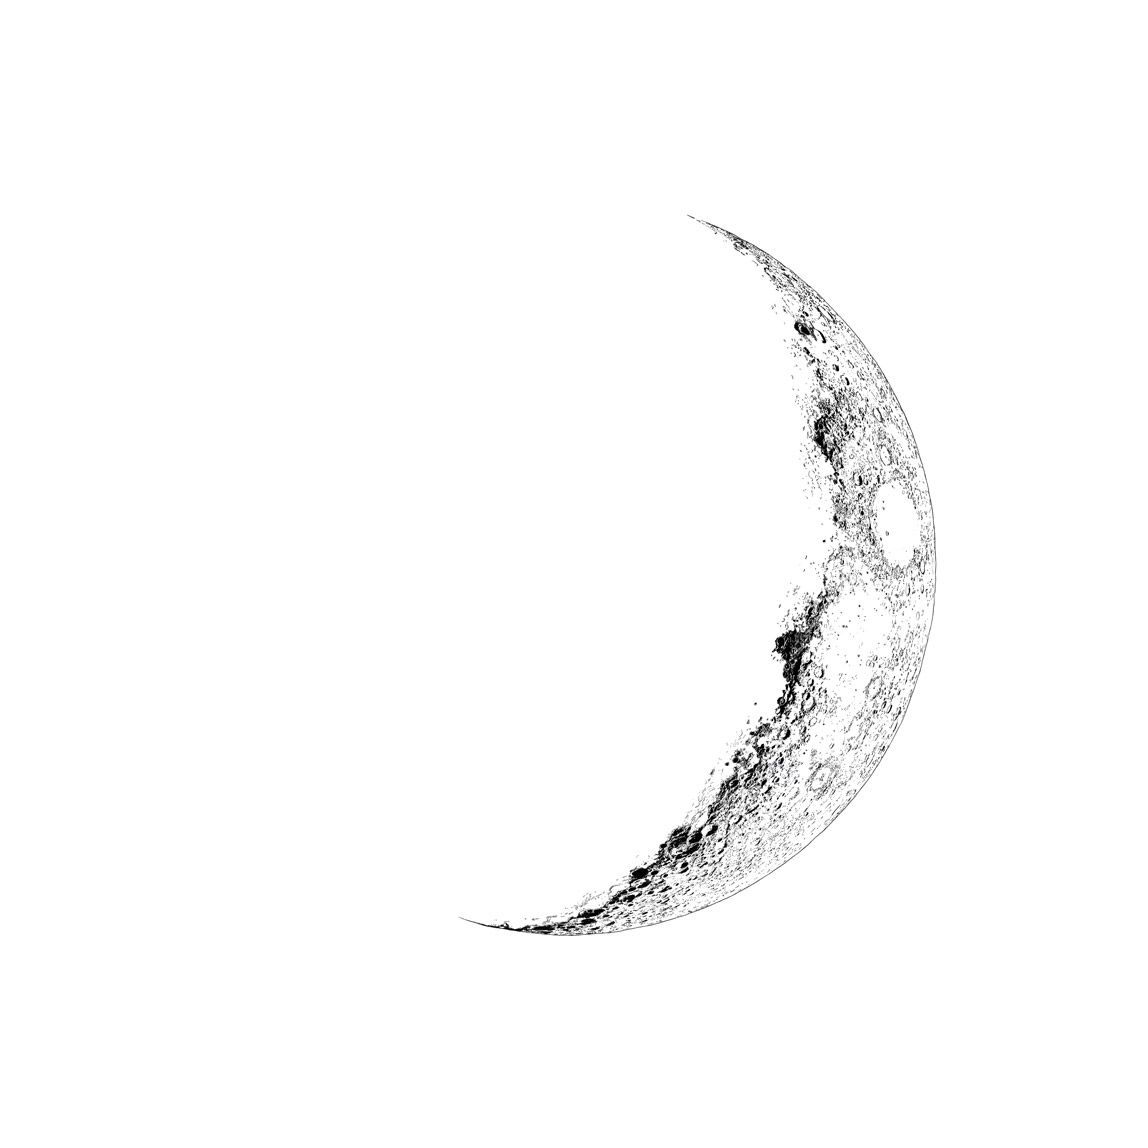
\includegraphics[width=\paperheight]{moon.jpg}
%  }%
%}


\usepackage[pages=some]{background}
\backgroundsetup{
scale=0.9,
color=black,
opacity=0.8,
angle=-30,
pages=some,
position={9cm, -7cm},
contents={%
  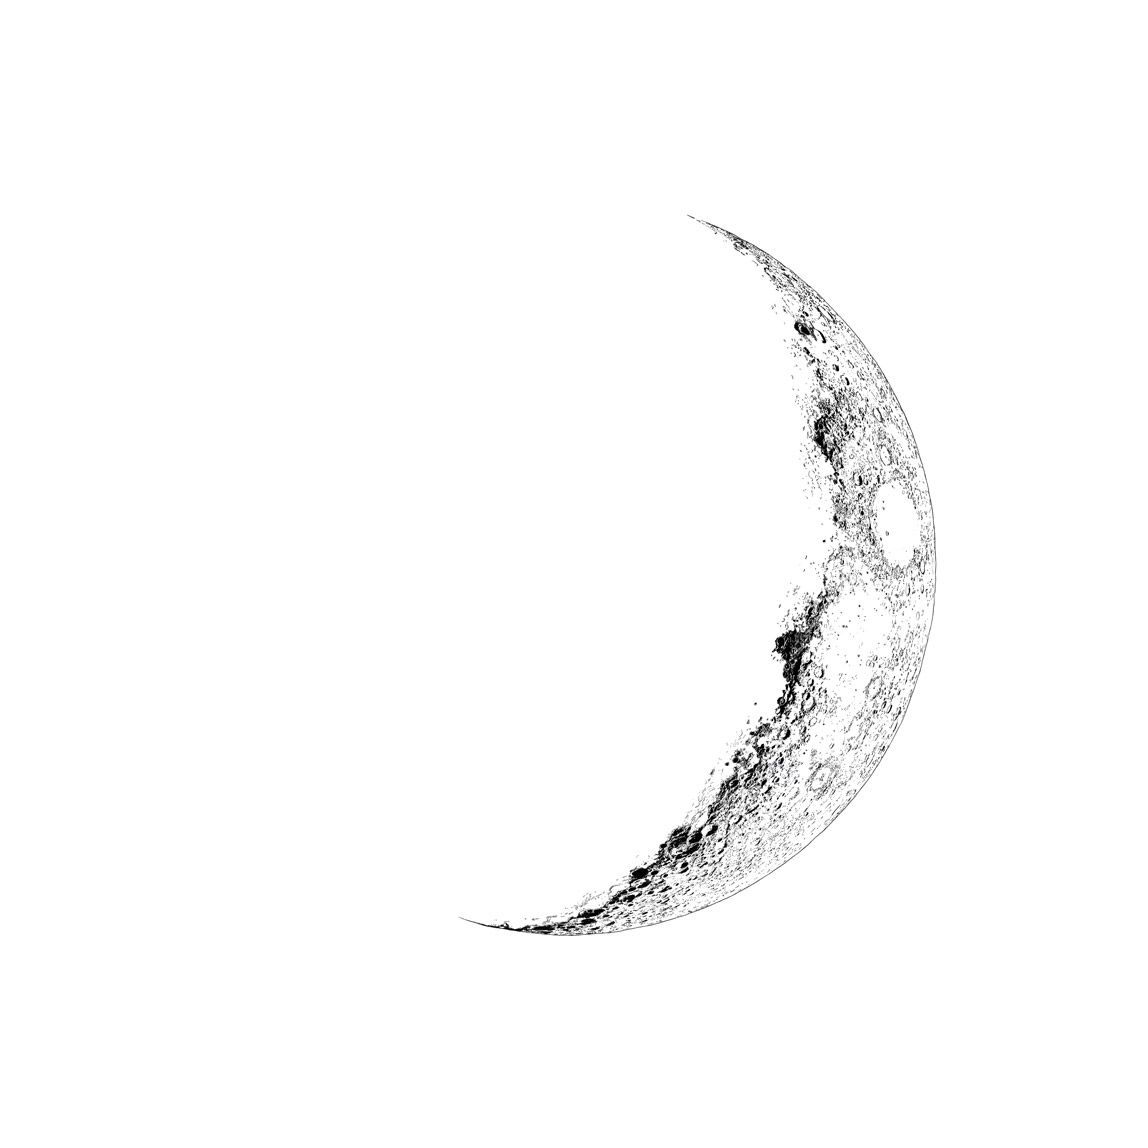
\includegraphics[width=\paperheight]{moon.jpg}
  }%
}

\begin{document}
%\BgThispage
\BgThispage
\RestyleAlgo{ruled}
\clearpage
%% temporary titles
% command to provide stretchy vertical space in proportion
\newcommand\nbvspace[1][3]{\vspace*{\stretch{#1}}}
% allow some slack to avoid under/overfull boxes
\newcommand\nbstretchyspace{\spaceskip0.5em plus 0.25em minus 0.25em}
% To improve spacing on titlepages
\newcommand{\nbtitlestretch}{\spaceskip0.6em}
\pagestyle{empty}
\begin{center}
\bfseries
\nbvspace[3]
\Huge
{\nbtitlestretch
{\normalsize CRAFTING A }\\
\Huge CONICAL REFRACTION \\
POLARIMETER }

\nbvspace[2]
{\small

TOWARDS A LOW-COST\vspace{0.2cm}\\  DEVICE TO MONITOR\vspace{0.2cm}\\ LINEAR POLARIZATION\\
}

\normalsize

\nbvspace[8]
\small BY\\
\Large Xabier Oyanguren Asua\\[0.5em]
%\footnotesize Can we really foresee the future of the Universe?"\\

\nbvspace[1]

\small THESIS SUPERVISOR \vspace{0.15cm}\\
\Large Alex Turpin Avilés

\nbvspace[0.2]


\includegraphics[width=1.8in]{UAB.png}
\normalsize
\vspace{-0.5cm}
%\small Thesis Directors: \\
%\nbvspace[0.2]
%\large Jordi Mompart Penina \\
%Xavier Oriols Pladevall\\
%\nbvspace[1]

%Universitat Autònoma de Barcelona\\
\large
%DEGREE FINAL DISSERTATION \\
\small
Bachelor's Thesis \\ \small Computational Mathematics and Data Analytics \\
\vspace{0.2cm}
\footnotesize 
2021-2022
\nbvspace[0.5]
\end{center}
\newpage
\null
\clearpage
\newpage
\begin{dedication}
Para Todor,\\ me debes una caña :)
\end{dedication}
\newpage
\null
\clearpage
\newpage
\clearpage
\maketitle
\vspace{-0.3cm}
\pagenumbering{gobble}
\setlength{\cftbeforesecskip}{0.4cm}
\setlength{\cftbeforesubsecskip}{0.4cm}
\setlength{\cftbeforesubsubsecskip}{0.25cm}

\tableofcontents
\clearpage
\newpage
\null
\clearpage
\newpage
\pagenumbering{arabic}
\setcounter{page}{1}
\vspace{-0.3 cm}

%\pagestyle{empty}
\pagestyle{fancy}

\section*{\centering \huge{Introduction}\vspace{-0.35cm}}
\noindent\rule{\textwidth}{0.4pt}
\addcontentsline{toc}{section}{Introduction}
\vspace{-0.8cm}
\section*{Abstract\vspace{-0.1cm}}
If one lights a biaxial crystal along its optical axis, the light beam opens in a conical shape and gets out as a hollow ring. This is known as Conical Refraction (CR). At each point along the ring, the light is linearly polarized, with an angle that rotates continuously as one moves along the ring. This happens irrespective of the input light's polarization state. Then, if the input was already linearly polarized, the ring component of its orthogonal polarization will have no light. The intensity continuously increases from there until the angular spot corresponding to the polarization angle of the input beam. This generates a crescent-moon-like shape, which encodes the linear polarization state of the input beam in the degree of rotation of the crescent moon relative to the crystal. This phenomenon was employed in \cite{Stokes1, Stokes2} to build a full Stokes polarimeter and in \cite{incomplete} for an (incomplete) polarimeter to measure changes in linear polarization. To do this a computer vision step is essential in order to convert the crescent rings into angle measurements. The computational solutions for this, offered in Refs. \cite{incomplete, Stokes1, Stokes2} were functional, but did not explore all the algorithmic landscape. In this work we will deeply explore the possible algorithms analyzing the theoretical symmetries and the experimental problems they face, in order to distill the best possible solution. With it, following the suggested hardware in Ref. \cite{incomplete}, after a small study, we build a functional proof-of-concept polarimeter with an integrated graphical user interface to measure variations of linear polarization in real time. We finally analyze its commercial viability.


%\section*{Objectives}\vspace{-0.2cm}

\section*{Guideline}\vspace{-0.1cm}
The present dissertation is divided into three parts. In part A we study the theoretical framework that allows the prediction of CR, both to have a deep understanding of the symmetries of the crescent rings that can be exploited in the algorithms, and to understand which ones are the experimental requirements of the device. Very importantly, this will provide us the means to simulate the phenomenon. Part A is the part that will be most interesting for the mathematician reader. (This part is heavily trimmed in the summarized version for it is a pedagogical revision of the essential theory).

 In part B, the core and main merit of the work, the previously unexplored algorithmic landscape is exhaustively walked through, by offering detailed solutions of very different nature, together with tips for their implementation. These are benchmarked in a big final test over the several datasets generated for the work. (This one will be the most interesting part for the computer-science reader.)

Finally, in Part C, we briefly review the experimental CR phenomenon and infer the practical blocks that should compose a polarimeter based on this phenomenon. With them, a proof-of-concept device is created, tested and compared with the current market options, looking for potential niches in which it could be industrially specialized. (This is the part that the engineer will enjoy the most).

\section*{Disclaimer on the Length of the Work\vspace{-0.1cm}}


Because the thesis could have an arbitrary number of pages, all the concepts and remarks required for completeness and to leave a self-contained dissertation were included. However, a summarized version was composed dedicated for the thesis qualifying board, which has multiple additional works to correct. Both works, together with all the generated computational material and results can be found in the project Github, Ref. \cite{github}.

\newpage

%%%%%%%%%%%%%%%%%%%%%%%%%%%%%%%%%%%%%%%%%%%%%%%%%%%%%%%%%%%%%%%%%%%%%%%%%%%%%%%%%%%%%%%%%%%%%%%%%%%%%%%%%%%%%%%%%%%%%%%%%%%%%%%%%%%%%%%%%%%%%%%%%%%%%%%%%%%%%%%%%%%%%%%%%%%%%
\newpage


%\begin{kapituloBerria}{Part A}{ Understanding the Underlying Phenomenon}
%Conical Refraction Essentials 
%\end{kapituloBerria}
%\newpage
%\fancyhead[L]{\null}
%\fancyhead[R]{\null}
%\null
%\clearpage
\newpage
\null
\clearpage
\newpage

\section*{\centering \huge{Part A: The Essence of the Polarimeter}\vspace{-0.4cm}}
\noindent\rule{\textwidth}{0.4pt}
\vspace{-0.4cm}
\addcontentsline{toc}{section}{Part A: 
The Essence of the Polarimeter}

In this first section, we will review the basic theoretical framework predicting the Conical Refraction (CR) phenomenon on which the developed polarimeter will be based. We will first derive the existence of the phenomenon from Maxwell's equations, by introducing all the notation and physics jargon that we will be employing throughout the work. We will then review the most complete description of the phenomenon so far, which will allow us to simulate it and generate theoretical predictions of what we will see in the laboratory. After noting the main features of a conically refracted beam, the idea underlying the intended polarimeter will emerge naturally.\vspace{-0.2cm}

\section*{A.1. Derivation of Conical Refraction from Maxwell's Equations\vspace{-0.2cm}}
\addcontentsline{toc}{subsection}{1. Derivation of Conical Refraction from Maxwell's Equations}
The following is a pedagogical introduction to crystal optics that will lead us to predict the CR phenomenon in a beautiful way, by only assuming the reader is familiar with Maxwell's equations. To write it, several text books were consulted, among them references \cite{LL,magnetostatic,fundamentals}.\vspace{-0.3cm}
\subsection*{A.1.1. Electromagnetic Waves \vspace{-0.2cm}}
Given we denote by $\vec{E}(\vec{r},t)$ and $\vec{B}(\vec{r},t)$ the electric and magnetic fields at the spatial position $\vec{r}=(x,y,z)\in\R^3$ and a given time $t\in\R$, their shape is given by the well known (microscopic) Maxwell's Equations, ruled by the electric charge density $\vec{\rho}(\vec{r},t)$ (charge per unit volume) and electric current density $\vec{J}(\vec{r},t)$ (charge density times the velocity field of its constituent particles):\vspace{-0.2cm}
\begin{equation}\label{div}
\vec{\nabla}_r\cdot \vec{E}(\vec{r},t)=\frac{1}{\varepsilon_0}\rho(\vec{r},t) \quad  \quad \quad \quad \vec{\nabla}_r\cdot \vec{B}(\vec{r},t)=0 \vspace{-0.2cm}
\end{equation}
\begin{equation}\label{curl}
\vec{\nabla }_r\cross \vec{E}(\vec{r},t)=-\pdv{\vec{B}(\vec{r},t)}{t}  \quad  \quad \quad \quad \vec{\nabla }_r\cross \vec{B}(\vec{r},t)=\mu_0\qty(\vec{J}(\vec{r},t)+\varepsilon_0\pdv{\vec{E}(\vec{r},t)}{t})\vspace{-0.2cm}
\end{equation}
where we define the "vector-operator" $\vec{\nabla}_r:=(\pdv{}{x}, \pdv{}{y},\pdv{}{z})$ and we denote by $\cdot$ the standard scalar vector product, while by $\cross $ the standard cross product. $\varepsilon_0$ and $\mu_0$ are some universal constants fixed to satisfy experiments (the electric {\bf permitivity} and the magnetic {\bf permeability of free space}, respectively). A separate law called the Lorentz force then rules the influence of these fields on the dynamics of the charge density and current.

The field curl equations \eqref{curl} for $\vec{E}$ and $\vec{B}$, relating the rate of change of each other, suggest that a time varying electric field must imply a time varying magnetic field, even if we consider a region of space with no charges $\rho\equiv 0$ and no currents $\vec{J}\equiv\vec{0}$, so called {\bf free space}. This suggests a "self-sustained" wave that could travel even in the vacuum of space (unlike other kinds of waves which propagate through a material medium) could exist. Indeed, we can take the curl $\vec{\nabla}_r\cross$ of the equations in \eqref{curl} and assuming no free charges nor currents, after using also equations \eqref{div}, we arrive to:\vspace{-0.2cm}
\begin{equation}\label{waveeq}
\mu_0\varepsilon_0\pdv[2]{\vec{E}(\vec{r},t)}{t}-|\vec{\nabla}_r|^2\vec{E}(\vec{r},t)=0 \quad \quad \quad \mu_0\varepsilon_0\pdv[2]{\vec{B}(\vec{r},t)}{t}- |\vec{\nabla}_r|^2\vec{B}(\vec{r},t)=0 \vspace{-0.2cm}
\end{equation}
where given a vector $\vec{v}=(v_x,v_y,v_z)$, $|\vec{v}|^2:=v_x^2+v_y^2+v_z^2$. We can identify these two equations with the classical wave equation by defining the constant $c:=\frac{1}{\sqrt{\varepsilon_0\mu_0}}$, known as the speed of light, to be the speed at which the wavefronts of the fields travel. This is the prove that an electric and magnetic field can indeed travel in free space as waves. Such a coupled pair of waves is called an {\bf electromagnetic wave}. Light turns out to be a wave of this kind.

From the equations \eqref{div} in free space, we can further restrict what an electromagnetic wave looks like. Consider the pair of waves $\vec{E}(\vec{r},t)=\vec{E}_0f(\vec{r}\cdot \hat{k}-ct)$ and $\vec{B}(\vec{r},t)=\vec{B}_0f(\vec{r}\cdot \hat{k}-ct)$ with a certain unit vector $\hat{k}$ and constant $\vec{B}_0,\vec{E}_0$. It is easy to see that all the $\vec{r}$ points in a same orthogonal plane to $\hat{k}$ have the same value of the vector fields. These same values $\vec{E}_0f$ and $\vec{B}_0f$ on the same plane travel along the direction $\hat{k}$ at a speed $c$. Thus, they are called traveling {\bf plane waves}. It is simple to verify that they satisfy both wave equations for an arbitrary second differentiable function $f(s)$. Then, introducing them in \eqref{div}, we get that $\hat{k}\cdot\vec{E}f'(\vec{r}\cdot \hat{k}-ct)=0$ and $\hat{k}\cdot\vec{B}f'(\vec{r}\cdot \hat{k}-ct)=0$. These mean that for a non-trivial $f$, it will need to happen that the electric and magnetic fields oscillate in the orthogonal plane to the propagation direction. Finally, using the first equation in $\eqref{curl}$ for such an {\em ansatz}, we get that $\hat{k}\cross \vec{E}_0 =c \vec{B}_0$, meaning that the electric and magnetic fields will need to be orthogonal to each other and that $|\vec{E_0}|=c|\vec{B}_0|$. This means that for a plane wave, if we only describe the electric field we will have enough for a full description of the magnetic field. 

Arbitrary {\bf sinusoids} moving in the spatial direction $\hat{k}:=\vec{k}/|\vec{k}|$ with an spatial angular frequency $|\vec{k}|$ and temporal angular frequency $w$, $f(\vec{r},t;\vec{k},w):=Acos(\vec{k}\cdot \vec{r}-wt)+Bsin(\vec{k}\cdot \vec{r}-wt)$, are convenient functions that can be shaped as the described plane waves if we restrict $w(|\vec{k}|)=c|\vec{k}|$. Their convenience is due to the following observations:\vspace{-0.2cm}
\fancyhead[OL]{\em Part A: The Essence of the Polarimeter}
\fancyhead[ER]{\em Bachelor's Thesis: Conical Refraction Polarimeter}
\fancyhead[OR]{ Electromagnetic Waves }
\fancyhead[EL]{ Electromagnetic Waves}
\begin{itemize}
\item A sinusoid is the shape that a field generated by an oscillating source could be expected to have far away from its generation point. Since electromagnetic waves are typically irradiated by oscillating charges, this happens to be the case.

\item Since for any $A,B\in\R$, we can find real $R=\sqrt{A^2+B^2}$ and $\phi=tan^{-1}(B/A)$ such that $Acos(d)+Bsin(d)=Rcos(d+\phi)$, we see that an arbitrary sinusoid that solves the above equations can always be rewritten as a cosine:
\begin{equation}
f(\vec{r},t;\vec{k},w)=Acos(\vec{k}\cdot \vec{r}-wt)+Bsin(\vec{k}\cdot \vec{r}-wt)=R\;cos(\vec{k}\cdot \vec{r}-wt+\phi)
\end{equation}
Now, since we have that such a sinusoid is equal to the real part of a complex exponential plane wave (which is what we will call in what follows a {\bf plane wave}):\vspace{-0.2cm}
\begin{equation}
R\;cos(\vec{k}\cdot \vec{r}-wt+\phi)=\mathfrak{R}e\{R^{i\phi}e^{i(\vec{k}\cdot \vec{r}-wt)}\}\vspace{-0.2cm}
\end{equation}
It is typical in optics to talk about complex plane waves when describing an electromagnetic wave. Since we only add electric fields and multiply them by real scalars in Maxwell's equations, we can in general manipulate a complex electric field, just by remembering that in the end we only care about what is encoded in the real part (discarding the imaginary one). This turns out to be very advantageous, among others, because differentiation can be trivially done, and as explained in the gray box below, it allows a simple management of the polarization of light, as adding a phase shift between sinusoidal vector components of the field, is reduced into multiplying a complex unit number to each component.

\item It turns out that solving how sinusoids evolve lets us know how any other acceptable initial conditions for the Maxwell Equations will evolve. To see this, first note that by the Fourier inversion theorem, an arbitrary well behaved real electric field $\vec{E}=(E_x,E_y,E_z)$ is decomposable as a continuous series of sinusoids or complex plane waves. That is, for each component of the electric field $E_j$ with $j\in\{x,y,z\}$ there will exist some real functions $R_j(\vec{k},t),\phi_j(\vec{k},t)$ such that:\vspace{-0.1cm}
\begin{equation}
E_j(\vec{r},t)={\small \frac{1}{(2\pi)^3}}\int_{\R^3} R_j(\vec{k},t)cos(\vec{k}\cdot\vec{r}+\phi_j(\vec{k},t))dk
=\mathfrak{R}e\qty{{\small\frac{1}{(2\pi)^3}}\int_{\R^3}R_j(\vec{k},t)e^{i\phi_j(\vec{k},t)}e^{i\vec{k}\cdot\vec{r}}dk}\vspace{-0.1cm}
\end{equation}
This means there will be a complex vector field $\vec{E}_0(\vec{k},w)=(\frac{1}{(2\pi)^3}R_j(\vec{k},t)e^{i\phi_j(\vec{k},t)}\big)_{j\in\{x,y,z\}}$ with:\vspace{-0.1cm}
\begin{equation}
\vec{E}(\vec{r},t)=\mathfrak{R}e\qty{\int_{R^3}\vec{E}_0(\vec{k},t)e^{i\vec{k}\cdot\vec{r}}dk}\vspace{-0.1cm}
\end{equation}
Plugging it into the wave equation \eqref{waveeq}, one gets:\vspace{-0.2cm}
\begin{equation}
-|\vec{k}|^2\vec{E}_0(\vec{k},t)-\frac{1}{c^2}\pdv[2]{\vec{E}_0}{t}=0
\end{equation}
which is solved by $\vec{E}_0(\vec{k},t)=\vec{E}_0(\vec{k},t=0)e^{\pm iwt}$ with $w=|\vec{k}|c$. This leaves:
\begin{equation}
\vec{E}(\vec{r},t)=\mathfrak{R}e\qty{\int_{\R^3}\vec{E}_0(\vec{k},t=0)e^{i(\vec{k}\cdot\vec{r}-wt)}dk}
\end{equation}
Meaning that if we know $\vec{E}_0(\vec{k},t=0)$, the Fourier decomposition coefficients for the initial electric field $\vec{E}(\vec{r},t=0)$, we will be able to know all its subsequent time evolution. This is a consequence of the fact that Maxwell's equations are linear: if two functions are solution to the equation, then any linear combination of them will also be a solution. Thus, if we have an initial condition that can be described as a linear combination of initial conditions for which the evolution is known, the time evolution of the objective initial conditions will be the "sum" of the evolution of its constituents. Moreover, we got that plane wave solutions of the electric field determine directly the magnetic field as well. Thus, by knowing the plane wave decomposition of the initial electric field we can immediately know the time evolution of the magnetic field $\vec{B}$ as well, even if the resulting electric and magnetic waves do not posses such a simple inter-relation.


\item A light beam with a well defined direction, energy and wavelength, like a laser beam, will be a combination of plane waves where a single wave-vector $\vec{k}$ and energy $w$ take the most significant weight in the Fourier decomposition. Thus, the behavior of a single sinusoid plane wave is a nice idealization of a light ray.

\end{itemize}

\mybox{{\bf The Polarization of Light \vspace{0.2cm}}\\
A transverse wave is a traveling wave that oscillates in a perpendicular direction to the wavefront propagation direction. The {\bf polarization} is then given by the pattern shaped by the transversally oscillating component of the wave. Since in the case of electromagnetic waves like the sinusoidal plane waves we described, the electric and magnetic field vectors (or the displacement and magnetization fields for anisotropic media) are always mutually orthogonal and orthogonal to the propagation direction, they are transverse waves and we can define a polarization state for them. In fact, their magnitudes are uniquely related by a constant, as we saw, so studying, say, the electric field's polarization will suffice. \\

For plane waves, we saw that the electric field vector will only have the freedom to oscillate in the orthogonal plane to the propagation direction. Thus, let us choose the z axis as the propagation direction, such tath the electric field $\vec{E}=E_x\hat{x}+E_y\hat{y}+E_z\hat{z}$ will have $E_z\equiv  0$, where $\hat{x},\hat{y},\hat{z}$ are the unit vectors of our Cartesian frame. Now, consider the sinusoid of frequencies $\vec{k},w$:
\begin{equation}
\vec{E}(\vec{r},t)=E_{0x}\ cos(\vec{k}\cdot\vec{r}-wt+\phi_x)\hat{x}+ E_{0y}\ cos(\vec{k}\cdot\vec{r}-wt+\phi_y)\hat{y}
\end{equation} 
with $E_{0x},E_{0y},\phi_x,\phi_y\in\R$ real degrees of freedom. The $x$ component of the net vector $\vec{E}$ is a cosine oscillating up and down in $\hat{x}$, while the $y$ component oscillates left-right in $\hat{y}$ at the same frequency in time and space as $x$, but possibly unsynchronized. This synchronization will be given by "how advanced" the cosine's oscillations are relative to each other. We call this relative argument distance, the {\bf relative phase} $\Delta \phi:=\phi_x-\phi_y$. Allowing $\Delta \phi$ to be any number we allow for a fixed $\vec{r},t$, the net vector $\vec{E}$ to point in any of the directions in the $xy$ plane. However, we realize that the traced shape by the vector $\vec{E}$ while $t$ or $\vec{r}$ advance, also depends on the {\bf relative magnitudes} $E_{0x}/E_{0y}$ of the components. For example, we know by only saying the relative phase is $\pi/2$ (such that the cosines are a quarter of period de-phased, coinciding the zero of one cosine with the maximum amplitude of the other), that the net electric vector will rotate in the $xy$ plane. The thing is that it will trace a perfect circle if $E_{0x}=E_{0y}$, while it will trace an ellipse otherwise (assuming $E_{0x},E_{0y}$ are non-zero). This ellipse will have its major axes oriented and scaled as a function of $E_{0x}/E_{0y}$. These two traced patterns or polarizations of a plane wave are called {\bf circular} and {\bf elliptical polarizations} (CP and EP) respectively, which can further be specified to be left- or right-handed, as a function of the direction of rotation. In fact, there is only one additional polarization state left. If either of $E_{0x},E_{0y}$ are zero, then the net vector will only oscillate in $x$ or $y$. If the relative phase is of any multiple of $\pi$ (the maximum amplitudes of the cosines coincide), then the net vector will also oscillate in a fixed plane. This is called {\bf linear polarization}. It is determined by the angle relative to the $x$ axis at which the vector oscillates. }
\mybox{ Since there are no more patterns a sinusoidal wave can take, we conclude that the state of polarization is uniquely determined by the relative phase and the relative magnitudes of the field components. In reality, light can also be unpolarized if it is a mixture of differently polarized plane waves, or randomly polarized if this mixture is stochastic, but we will not consider them in this work, since the input light will be something under our control.\vspace{-0.1cm}\\

 Lastly, we can gather in a single terms all the polarization information. We had that: $E_j(\vec{r},t)=E_{0j}cos(\vec{k}\cdot\vec{r}-wt+\phi_j)=\mathfrak{R}e\qty{E_{0j}e^{i\phi_j}e^{i(\vec{k}\cdot\vec{r}-wt)}}$ for all $j\in{x,y}$. We can factor out the exponential and the magnitude of the vector $E_0^2:=E_{0x}^2+E_{0y}^2$ to have:\vspace{-0.1cm}
\begin{equation}
\vec{E}(\vec{r},t)=\mathfrak{R}e\qty{\hat{u}_JE_0e^{i(\vec{k}\cdot\vec{r}-wt)} }\vspace{-0.1cm}
\end{equation}
Where $\hat{u}_J=\frac{1}{E_0}(E_{0x}e^{i\phi_x}\hat{x}+E_{0y}e^{i\phi_y}\hat{y})$ is a unit vector in $\C^2$ giving all the information about the polarization of the wave (the relative magnitude and phase). Because in general we do not care about the common cumulative phase of both components to know the polarization, we identify $\hat{u}_J$ with $e^{i\varphi}\hat{u}_J$ $\forall 	\varphi\in\R$.\footnote{It is interesting to note that this polarization state space is then equal to the space of representation of a two dimensional quantum system (a qubit). This, together with the fact that the most relevant classical optical devices are linear (they act as linear operators on the electric field), justify why light polarization is also employed as a "qubit" for quantum experiments.} This "neglected" multiplicative factor is called a {\bf global phase}. The unit vector $\hat{u}_J$ is called the {\bf Jones vector} or polarization vector.\vspace{-0.1cm}\\

Note that working with complex plane waves is very useful also because now, adding a relative phase shift between the components of polarization is just about multiplying a unit complex number to one component of the Jones vector. This means that if we allow linear operations on the electric field to be over complex coefficients (taking the real part after the operation), we will be able to easily play with the relative phases and the polarization as well. For all this practicality, in the remaining we will assume the real part operation for electric field plane waves and {\bf we will omit the explicit $\mathfrak{R}e\{\}$ operation}.
}\vspace{-0.5cm}

\subsection*{A.1.2. An Anisotropic Medium for Light\vspace{-0.2cm}}
\fancyhead[OR]{ An Anisotropic Medium for Light}
\fancyhead[EL]{ An Anisotropic Medium for Light}
One could think this convenient description of light as an electromagnetic wave, where we only need to specify the electric field for sinusoidal plane waves will not be useful once we introduce other charges than the ones that generated the electromagnetic field in a far away spot. Yet, it turns out that the propagation of light in linear dielectric materials, can still be described as a wave traveling, now, through a "modified vacuum". 

Inside a material, there are electron clouds bound to their nuclei. Electric fields cause a displacement on such bound clouds generating microscopic dipoles (charge separations) within each atom. All these dipoles can statistically be averaged to make macroscopically significant bound charge separations. These must be taken into account in macroscopic scale Maxwell's equations. In fact, if the material has less bound electrons (like metals do), their effect will be even more dramatic. On the other hand, all electrons bound to a nuclei have intrinsic angular momentum (due to spin and orbital angular momentum), which imply microscopic charge currents (or magnetic dipoles) generating magnetic fields. These can align and cause an average macroscopic current effect. Again, even more notorious will be the effect of unbound electrons. Then, inside a material, in general there will be two contributions to the total electric and magnetic fields: the one due to the bound charge- and current-densities $\rho_b$ and $\vec{J}_b$ and the one due to the rest of charges and currents (including the external fields) $\rho_f$ and $\vec{J}_f$. Let us define a bound charge electric field as the field generated by bound charge densities $\vec{\nabla}\cdot \vec{E}_b=\frac{1}{\varepsilon_0}\rho_b$, while a bound magnetic field as the one implied by the bound currents and the bound electric field: $\vec{\nabla}\cross \vec{B}_b=\vec{J}_b+\varepsilon_0\pdv{\vec{E}_b}{t}$. By the linearity of Maxwell's equations, we can write the total fields as the sum of these fields and the fields generated by the rest of (freer) charges as: $\vec{E}=\vec{E}_b+\vec{E}_f$ and $\vec{B}=\vec{B}_b+\vec{B}_f$. This expands Maxwell's equations as:
\begin{equation}\label{divBt}
\vec{\nabla}_r\cdot \vec{E_f}(\vec{r},t)=\frac{1}{\varepsilon_0}\rho_f(\vec{r},t) \quad  \quad\vec{\nabla}_r\cdot \vec{E_b}(\vec{r},t)=\frac{1}{\varepsilon_0}\rho_b(\vec{r},t) \quad \quad \vec{\nabla}_r\cdot \vec{B}_f(\vec{r},t)=0 \quad \quad \vec{\nabla}_r\cdot \vec{B}_b(\vec{r},t)=0 
\end{equation}
\begin{equation}\label{curlBt}
\vec{\nabla }_r\cross \vec{E}(\vec{r},t)=-\pdv{\vec{B}(\vec{r},t)}{t} 
\end{equation}
\begin{equation}\label{anotherone}
\vec{\nabla }_r\cross \vec{B}_f(\vec{r},t)=\mu_0\qty(\vec{J}_f(\vec{r},t)+\varepsilon_0\pdv{\vec{E}_f(\vec{r},t)}{t})\quad \quad  \vec{\nabla }_r\cross \vec{B}_b(\vec{r},t)=\mu_0\qty(\vec{J}_b(\vec{r},t)+\varepsilon_0\pdv{\vec{E}_b(\vec{r},t)}{t})
\end{equation}

The reason for this equation multiplication will be clear in a moment. In general, we are not interested in the microscopic description of the bound charges. Instead, phenomenological relations are employed to describe their contribution in a total electric and magnetic field $\vec{E}$, $\vec{B}$. For so called {\bf linear materials}, these bound charge contributions are describable as a linear transformation of the total fields: $\vec{E}_b=-\pmb{\chi_e} \vec{E}$ and $\pmb{\chi}\vec{B}_b= \vec{B}$ with $\pmb{\chi}:=\pmb{Id}+\pmb{\chi_m^{-1}}$, where $\pmb{\chi_e}$ and $\pmb{\chi_m}$ are material specific non-singular matrices called the electric and magnetic {\bf susceptibilities}. $\pmb{(\cdot)^{-1}}$ denotes matrix inversion and $\pmb{Id}$ is the identity matrix\footnote{If the material has an {\bf homogeneous} crystal structure, then these operators will be equal in all its inner points. However, we could also describe an inhomogeneous linear medium, by letting them depend on space and time. }. 

Since the bound charges and currents manifest themselves as averaged electric and magnetic dipole moments, it is typical to describe their generated fields $\vec{E}_b$ and $\vec{B}_b$ in dipole-moment density units (say, charge times displacement densities for the electric case). This can be done by just scaling the fields with the permitivity and permeability constants of free space $\varepsilon_0,\mu_0$. If so, we get $\vec{P}:=-\varepsilon_0\vec{E}_b$ and $\vec{M}:=\frac{1}{\mu_0}\vec{B}_b$, called the {\bf polarization\footnote{Not to be confused with the polarization of light.} and magnetization fields}. In order to unify the units it is typical to describe the unbound charge fields as well in dipole-moment density units, by defining $\vec{D}:=\varepsilon_0\vec{E}_f$ and $\vec{H}:=\frac{1}{\mu_0}\vec{B}_f$, which are called the {\bf displacement and magnetizing fields} respectively.

Now, here comes the reason for the equation unfolding. By knowing the phenomenological susceptibilities $\pmb{\chi_e},\pmb{\chi_m}$, we need not solve all the the expanded Maxwell equations. We have enough with the unbound charge contributions $\vec{D},\vec{H}$ (which in certain materials do not require a microscopic description, as we will see), in order to get the total electric and magnetic fields $\vec{E},\vec{B}$. For this, we just miss having the total fields in their function:
\begin{equation}\label{def1}
\vec{E}=\vec{E}_f+\vec{E}_b \Longrightarrow \varepsilon_0\vec{E}=\vec{D}+\varepsilon_0\vec{E}_b\Longrightarrow \vec{D}=\varepsilon_0(\pmb{Id}+\pmb{\chi_e})\vec{E} \Longrightarrow \vec{D}=\pmb{\varepsilon}\vec{E}
\end{equation} 
where $\pmb{\varepsilon}:=\varepsilon_0(\pmb{Id}+\pmb{\chi_e})$ is an invertible matrix, specific to the material, relating the total and displacement fields, known as the {\bf electric permitivity of the medium}. Much the same way:
\begin{equation}\label{def2}
\vec{B}=\vec{B}_f+\vec{B}_b \Longrightarrow \frac{1}{\mu_0}\vec{B}=\vec{H}+\frac{1}{\mu_0}\vec{B}_b\Longrightarrow \vec{B}=\mu_0(\pmb{Id}+\pmb{\chi_m})\vec{H}\Longrightarrow \vec{B}=\pmb{\mu} \vec{H}
\end{equation} 
where $\pmb{\mu}:=\mu_0(\pmb{Id}+\pmb{\chi_m})$ is an invertible matrix specific to the material, relating the total and magnetizing fields, known as the {\bf magnetic permeability of the medium}. Both matrices can be chosen to be complex in order to model a dephasing with the input field and absorption by the medium.

\noindent All this allow us to rewrite the microscopic Maxwell's equations or {\small \eqref{divBt},\eqref{curlBt},\eqref{anotherone}} as four equations: 
\begin{equation}\label{div2}
\vec{\nabla}\cdot \vec{D}=\rho_f \quad \quad \quad \quad \quad \quad \vec{\nabla}\cdot \vec{H}=0
\end{equation}
\begin{equation}\label{curl2}
\vec{\nabla}\cross \vec{E}=-\pdv{\vec{B}}{t} \quad \quad \quad \quad \quad \quad \vec{\nabla}\cross \vec{H}=\vec{J}_f+\pdv{\vec{D}}{t}
\end{equation}
plus the two {\bf constitutive equations} \eqref{def1} and \eqref{def2}. Together, these six equations are called the {\bf macroscopic Maxwell's equations}, that safe us the explicit microscopic modeling of bound charges.

An additional reason to rewrite them this way is because these equations have a similar look to the microscopic Maxwell's equations \eqref{div}, \eqref{curl} for $\vec{D},\vec{H}$. Indeed, let us consider a linear and homogeneous material with the susceptibilities, and thus $\pmb{\varepsilon},\pmb{\mu}$, being constant scalars $\varepsilon,\mu$ within the material (the three eigenvalues of the susceptibilities are the same constants), what we call an {\bf isotropic material}. We would see that the first equation in \eqref{curl2} would become in $\vec{\nabla}\cross\vec{D}=-\varepsilon\mu\pdv{\vec{H}}{t}$, which would now leave a system exactly the same as the microscopic Maxwell's equations but for $\vec{D},\vec{H}$ (plus the constitutive phenomenological equations to get the full fields). In such a case, we see that if we consider a {\bf dielectric material}: meaning that there is no free charge (most crystals used in optics), inside the material the free charge density and current will be null (only bound charges and currents will be present). Thus, by taking the curl of the equations in \eqref{curl2} as we did in free space, we would arrive to two equations:
\begin{equation}
\varepsilon\mu\pdv[2]{\vec{D}(\vec{r},t)}{t}-|\vec{\nabla}_r|^2\vec{D}(\vec{r},t)=\vec{0} \quad \quad \quad \varepsilon\mu\pdv[2]{\vec{H}(\vec{r},t)}{t}-|\vec{\nabla}_r|^2\vec{H}(\vec{r},t)=\vec{0}
\end{equation}
where we recognize again classical wave equations, just that now the propagation speed of the wavefronts is $\frac{1}{\sqrt{\varepsilon\mu}}$ instead of $c={1}/{\sqrt{\varepsilon_0\mu_0}}$. For the rest of matters, such an isotropic material would behave as free space, with the same consequences for the description of self-sustained electromagnetic waves in terms of $e^{\vec{k}\cdot\vec{r}-wt}$ plane aves.

That was very convenient. In reality however, we know that most crystals show a different light propagation as a function of the propagation direction. This is because, their susceptibilities $\pmb{\chi_e},\pmb{\chi_m}$ are not scalars. These are called {\bf anisotropic materials}. In these materials we are no longer able to obtain a classical wave equation (since curl and matrix multiplication do not commute), but we can still prove that for {\bf dielectric materials} (no free charges nor currents), plane wave solutions that satisfy our intuitions for light in free space still exist. In particular, let us assume solutions $\vec{D}=\vec{D}_0e^{\vec{k}\cdot\vec{r}-wt}$ and $\vec{H}=\vec{H}_0e^{\vec{k}\cdot\vec{r}-wt}$ with $\vec{D}_0,\vec{H}_0\in\C^3$ arbitrary complex constants. Note we leave the speed of propagation of the equal-phase-planes $v=w/|\vec{k}|$ as a free parameter that will be fixed by the equations later on. We first observe that since $\vec{E}=\pmb{\varepsilon^{-1}}\vec{D}$ and $\vec{B}=\pmb{\mu}\vec{H}$, if $\vec{D}$ and $\vec{H}$ are plane waves, then: $\vec{E}=e^{\vec{k}\cdot\vec{r}-wt}\pmb{\varepsilon^{-1}}\vec{D}_0$ and $\vec{B}=e^{\vec{k}\cdot\vec{r}-wt}\pmb{\mu}\vec{H}_0$ will also be plane waves with the same frequencies, even if they will not satisfy the following important intuition for light. By plugging $\vec{D}$ and $\vec{H}$ in \eqref{div2}, we have that $\vec{k}\cdot\vec{D}=0$,  $\vec{k}\cdot\vec{H}=0$: the propagation direction $\vec{k}$ will need to be orthogonal to the oscillation directions $\vec{D}_0,\vec{H}_0$. Thus, hey are transverse waves. $\vec{B}$ must also satisfy this, but $\vec{E}$ need not.

 On the other hand, plugging these plane wave {\em ansatze} in \eqref{curl2}, we find:\vspace{-0.1cm}
\begin{equation}\label{Fcurl}
\vec{k}\cross\vec{E}=w\vec{B} \quad \text{           and           }\quad  \vec{k}\cross\vec{H}=-w\vec{D}\vspace{-0.1cm}
\end{equation}  
These mean that $\vec{E}$ and $\vec{B}$ are orthogonal to each other and $\vec{H}$ and $\vec{D}$ as well (which are also orthogonal to the propagation direction). Also, noting that $v:=w/|\vec{k}|$ is the plane wave's equal-phase-plane transport speed, known as {\bf phase velocity}, the last equations imply $|\vec{H}_0|=v|\vec{D}_0|$ and $|\vec{E}_0|=v|\vec{B}_0|$. These together mean that $|\pmb{\varepsilon^{-1}}\vec{D}_0|=v|\pmb{\mu}\vec{H}_0|$ (which for isotropic media would yield $v^2=\frac{1}{\varepsilon\mu}$). Thus, we still have that plane waves solve Maxwell's equations in a way that the "magnetic part" is completely determined by the "electric part". So, practically, our intuitions are intact (for $\vec{D}$ and $\vec{H}$ especially). \vspace{-0.2cm}

\subsection*{A.1.3. The Dispersion Relation in an Anisotropic Dielectric Medium\vspace{-0.2cm}}
\fancyhead[OR]{The Dispersion Relation in Anisotropic Medium}
\fancyhead[EL]{The Dispersion Relation in Anisotropic Medium}
We just miss the question of how $w$ and $\vec{k}$ are mutually restricted for plane waves to be solutions of the macroscopic Maxwell's equations. This restriction is called the {\bf dispersion relation}. Equivalently, we want to know which is the spatial frequency $|\vec{k}|$ for a plane wave with temporal frequency $w$ or the phase propagation speed $v=w/|\vec{k}|$. The ratio of this speed to the free space speed $n:=c/v=c|\vec{k}|/w$ is called the {\bf refractive index}. Answering this question is how we will arrive to conical refraction. For this, retake equations \eqref{Fcurl} and plug in the constitutive equations \eqref{def1} and \eqref{def2} to get:
\begin{equation}\label{honek}
\vec{k}\cross \vec{E}=w\pmb{\mu}\vec{H} \quad \quad \quad \vec{k}\cross\vec{H}=-w\pmb{\varepsilon}\vec{E}
\end{equation} 
If we now define the operation of cross product with $\vec{k}=(k_x,k_y,k_z)\in\R^3$ as:\vspace{-0.1cm}
\begin{equation}
\pmb{k}:=\begin{pmatrix}
0& -k_z& k_y\\
k_z & 0 & -k_x\\
-k_y & k_x & 0
\end{pmatrix}\vspace{-0.1cm}
\end{equation}
such that $\vec{k}\cross\vec{a}=\pmb{k}\;\vec{a}$ for any $\vec{a}\in\C^3$, using the inverses of $\pmb{\varepsilon}$,$\pmb{\mu}$ and applying $\pmb{k}$ in each side of equations \eqref{honek}, we can rewrite them as:\vspace{-0.1cm}
\begin{equation}
\qty[\pmb{k}\pmb{\varepsilon^{-1}}\pmb{k}+w^2\pmb{\mu}]\vec{H}=\vec{0} \quad \quad \quad \qty[\pmb{k}\pmb{\mu^{-1}}\pmb{k}+w^2\pmb{\varepsilon}]\vec{E}=\vec{0}
\end{equation}
These are the so called {\bf complex vector wave equations} for anisotropic media. For a non trivial solution ("not all zero") to exist, the determinant of the matrices preceding $\vec{H}$ and $\vec{E}$ must be zero:
\begin{equation}\label{wave2}
det\qty(\pmb{k}\pmb{\varepsilon^{-1}}\pmb{k}+w^2\pmb{\mu})=0 \quad \quad\quad det\qty(\pmb{k}\pmb{\mu^{-1}}\pmb{k}+w^2\pmb{\varepsilon})=0
\end{equation}
Since the matrices $\pmb{\mu}$ and $\pmb{\varepsilon}$ are known, these equations will give the restriction relating the allowed plane wave $\vec{k}$ and $w$ for this medium: the dispersion relation $w(\vec{k})$. In reality both equations must be equivalent conditions, since both $\vec{H}$ and $\vec{E}$ must coexist, so we can choose the simplest one of them as a function of how difficult the inversion of $\pmb{\mu}$ and $\pmb{\varepsilon}$ are.

In our case, we will choose to study crystals that {\bf barely have magnetic response}, which are the typical ones employed in optical elements. This will mean that $\pmb{\mu}\simeq \mu_0\pmb{Id}$. As such, the simplest equation to develop the dispersion relation will be the second one in \eqref{wave2}. Let us choose the reference frame in which the coordinate axes are aligned with the eigenvectors of $\pmb{\varepsilon}$ (which can be chosen to be orthogonal for it can be proven that $\pmb{\varepsilon}$ must be Hermitian). By defining the ordered eigenvalues of $\pmb{\varepsilon}$ as $\varepsilon_x, \varepsilon_y, \varepsilon_z$, it is easy to get from the second equation of \eqref{wave2} with $\vec{k}=(k_x,k_y,k_z)$:
\begin{equation}
det\begin{pmatrix}
w^2\mu_0\varepsilon_x-(k_y^2+k_z^2) & k_xk_y & k_xk_z\\
k_yk_x & w^2\mu_0\varepsilon_y-(k_z^2+k_x^2) & k_yk_z\\
k_xk_z & k_yk_z & w^2\mu_0\varepsilon_z-(k_x^2+k_y^2)
\end{pmatrix}=0
\end{equation}
which after developing the equation, dividing by $w^2$ and by $\mu_0$ both sides and multiplying the whole by $c^6\mu_0$, leads to the next equation, grouping by $w$:
\begin{equation}\label{Fres}
w^4\varepsilon_x\varepsilon_y\varepsilon_z-w^2c^2\qty[k_x^2\varepsilon_x(\varepsilon_y+\varepsilon_z)+k_y^2\varepsilon_y(\varepsilon_x+\varepsilon_z)+k_z^2\varepsilon_z(\varepsilon_x+\varepsilon_y) ]+|\vec{k}|^2c^4\qty[\varepsilon_xk_x^2+\varepsilon_yk_y^2+\varepsilon_zk_z^2]=0
\end{equation}
For a given constant $w$, this is a fourth order surface in the possible wavevector $\vec{k}=(k_x,k_y,k_z)$ space, known as {\bf Fresnel's surface}. It can readily be seen that by fixing a certain $w$, and given the direction of $\vec{k}$, just leaving its magnitude $|\vec{k}|^2$ as unknown, equation \eqref{Fres} is a quadratic equation with real coefficients. This means, in general there will be two possible spatial frequencies $|\vec{k}|$, thus two possible phase velocities $v=w/|\vec{k}|$ and two possible refractive indices $n=c/v$, for each given direction in $k$-space. This is opposed to the isotropic medium or free space plane waves, where there was only a single acceptable wavelength and refractive index per $w$. This is why for material mediums where at least one of the eigenvalues of $\pmb{\varepsilon}$ is different to the rest, if a single light ray hits the crystal, it will propagate inside (refract) typically as two light rays with different refractive indices. This phenomenon is known as {\bf birefringence}. This is not always the case yet: Fresnel's surface has some singular directions where there is only a single allowed refractive index (only one solution $|\vec{k}|$). This will turn out to yield the prediction of conical refraction. For this however, we miss a last little step: we need to realize that the constant $w$ surfaces for the function $w(\vec{k})$, implicitly defined in \eqref{Fres}, also tell us the direction in which an actual physical light ray (composed of many plane waves) will propagate.

\mybox{{\bf Group Velocity\vspace{0.2cm}}\\
Plane waves are very unrealistic since they have an infinite extent in space and time. Instead, we could write a more general finite extent field following the general Fourier integral as a (continuous) superposition of plane waves:\vspace{-0.2cm}
\begin{equation}
\vec{D}(\vec{r},t)= \frac{1}{(2\pi)^4}\int_{\R^4}\hat{\vec{D}}(\vec{k},w)e^{i(\vec{k}\cdot\vec{r}-wt)}\; dw\;dk_x\;dk_y\;dk_z
\end{equation}}
\mybox{
We already saw that not all $w$ and $\vec{k}$ pairs are allowed, which had to follow $w(\vec{k})$ implicitly defined in \eqref{Fres}. Thus in reality:\vspace{-0.2cm}
\begin{equation}
\vec{D}(\vec{r},t)= \frac{1}{(2\pi)^3}\int_{\R^3}\hat{\vec{D}}(\vec{k})e^{i(\vec{k}\cdot\vec{r}-w(\vec{k})t)} \;dk_x\;dk_y\;dk_z\vspace{-0.2cm}
\end{equation}
Now, typically a light ray, say a laser beam, is very monochromatic, having a sharply defined wavelength $\lambda_c$, and has a defined phase propagation direction $\hat{k_c}$ (unit vector). This implies there is a dominant plane wave in its decomposition: the wave-vector $\vec{k}_c=\frac{2\pi}{\lambda_c}\hat{k}_c$. If so, the Fourier coefficients $\hat{\vec{D}}(\vec{k})$ will be sharply peaked around $\vec{k}_c$, making only $\vec{k}$ around $\vec{k}_c$ relevant. This implies, we could consider only the first two terms of the Taylor series of $w(\vec{k})$ around $\vec{k}_c$:\vspace{-0.2cm}
\begin{equation}
w(\vec{k})\simeq w(\vec{k}_c)+\vec{\nabla}_kw(\vec{k})\Big\rvert_{\vec{k}_c}\cdot\qty(\vec{k}-\vec{k}_c)+\cdots\vspace{-0.2cm}
\end{equation}
By writing $\vec{k}=\vec{k}_c+(\vec{k}-\vec{k}_c)$, we can rewrite the Fourier expansion as:\vspace{-0.1cm}
\begin{equation}
\vec{D}(\vec{r},t)=e^{i(\vec{k}_c\cdot\vec{r}-w(\vec{k_0})t)}\int_{\R^3}\hat{\vec{D}}(\vec{k})\;e^{i\qty((\vec{k}-\vec{k}_c)\cdot [\vec{r}-\vec{\nabla}_kw(\vec{k}_c)t])}\;dk_x\;dk_y\;dk_z\vspace{-0.2cm}
\end{equation}
The integral varies very slowly in space compared with the factored out plane wave, which has a very high frequency in space $|\vec{k}_c|$ compared with the relevant plane waves for the integral, since we assumed  $|\vec{k}-\vec{k}_c|<<|\vec{k}_0|$. We realize in consequence that the factored out plane wave is a fast sinusoid that is modulated by the slowly varying envelope integral. As such, in order to know the direction of motion of the light packet, we will need to see the direction in which the envelope is moving. We can fix our attention in a particular point of the moving envelope by tracking the trajectory traced by a fixed value of the integral. That is, the envelope follows the same trajectory as the the one traced by a fixed value for $\vec{r}-\vec{\nabla}_kw(\vec{k}_c)t=c$, with a fixed constant $c$. We can then get the velocity vector for the displacement of this fixed point of the envelope with a time derivative:
\begin{equation}
\vec{v}_g(\vec{k}_c)=\vec{\nabla}_kw(\vec{k})\Big\rvert_{\vec{k}_c}
\end{equation}
We call $\vec{v}_g(\vec{k})$ the {\bf group velocity} of the light ray of main frequency $\vec{k}$
}

Thus, a light ray of main frequency $\vec{k}$ will propagate in space in the direction of the gradient of $w(\vec{k})$, which geometrically implies it will move following the orthogonal vector to the tangent plane of the constant $w$ Fresnel surface level of $w(\vec{k})$. Note interestingly that a plane wave may have a phase velocity vector (pointing in the direction in which equal-phase-planes or wavefronts flow) $\vec{v}(\vec{k})=w/|\vec{k}|^2\vec{k}$ that is different to the actual propagation direction of its composed beam $\vec{v}_g(\vec{k})=\vec{\nabla}_kw(\vec{k})$, both in magnitude and direction\footnote{It can be proven, following the intuition for a moving wave-packet that the direction of energy flow naturally matches the group velocity's direction.}. This "sideways-walking" rays are called {\bf extraordinary rays} (for they will not obey exactly Snell's law).\vspace{-0.2cm}

\subsection*{A.1.4. Hamilton's Diabolical Singularity and Conical Refraction\vspace{-0.2cm}}
\fancyhead[OR]{Hamilton's Diabolical Singularity and Conical Refraction}
\fancyhead[EL]{Hamilton's Diabolical Singularity }
There are three types of crystals as a function of their electric permitivity $\pmb{\varepsilon}$. If the three eigenvalues $\varepsilon_x=\varepsilon_y=\varepsilon_z$ are equal, the medium is isotropic (as we explained). This happens if the crystal has a cubic lattice. If there is one eigenvalue that is different to the other two $\varepsilon_{xy}:=\varepsilon_x=\varepsilon_y\neq \varepsilon_z$, then the crystal is called {\bf uniaxial}. These are due to rhombohedral, tetrahedral and hexagonal crystal lattices, which have a main symmetry axis matching the eigenvector of $\varepsilon_z$, called the {\bf optical axis} of the crystal. If we plug these $\varepsilon_j$ in Fresnel's equation \eqref{Fres}, it factors as: $(k^2c^2-w^2\varepsilon_{xy})\qty(c^2(\varepsilon_zk_z^2+\varepsilon_{xy}(k_x^2+k_y^2))-w^2\varepsilon_z\varepsilon_{xy})=0$, which is solved by the two quadratic equations:
\begin{equation}
\frac{k_x^2+k_y^2+k_z^2}{\varepsilon_{xy}}=\frac{w^2}{c^2} \quad \quad \quad \frac{k_z^2}{\varepsilon_{xy}}+\frac{k_x^2+k_y^2}{\varepsilon_z}=\frac{w^2}{c^2}
\end{equation}
These are the equation of a sphere and an ellipsoid, where one of the semi-axes of the ellipsoid matches the radius of the sphere. It is depicted for a fixed $w$ in Figure \ref{fig:concentric1}.a. This means that there is one axis in the crystal (the eigenspace of $\varepsilon_z$, the $z$ axis in the Figure), along which for a fixed $w$, there is only one allowed $\vec{k}$. For all the rest of directions, two $\vec{k}$ exist (the green and the pink surfaces). By translational symmetry along an {\bf interface} between two mediums, given an input plane wave of vector $\vec{k}_{in}$ crossing it, the tangent component to the interface must be conserved (the same goes for $w$ by time translational symmetry). Thus, we can know which ones will be the $\vec{k}$ vectors of this ray inside the crystal (refraction), by looking at the allowed $\vec{k}$ that have the same tangent components (see Figure \ref{fig:concentric1}.b). For the shape of the Fresnel surface, unless the input ray was directed along the optical axis, it will be refracted with two different $\vec{k}$, phase velocities or refractive indexes (birefringence). In fact, because the tangent planes to the sphere and the ellipse have a different normal, and the normal was shown to give the direction in which a physical light ray propagates, we see that the input beam will be refracted into two beams propagating in different directions. The ellipsoid one will be an extraordinary ray. Thus, these crystals are called uniaxial because they have a single axis along which no birefringence occurs.\vspace{-0.3cm}

\begin{figure}[h!] 
     \centering 

    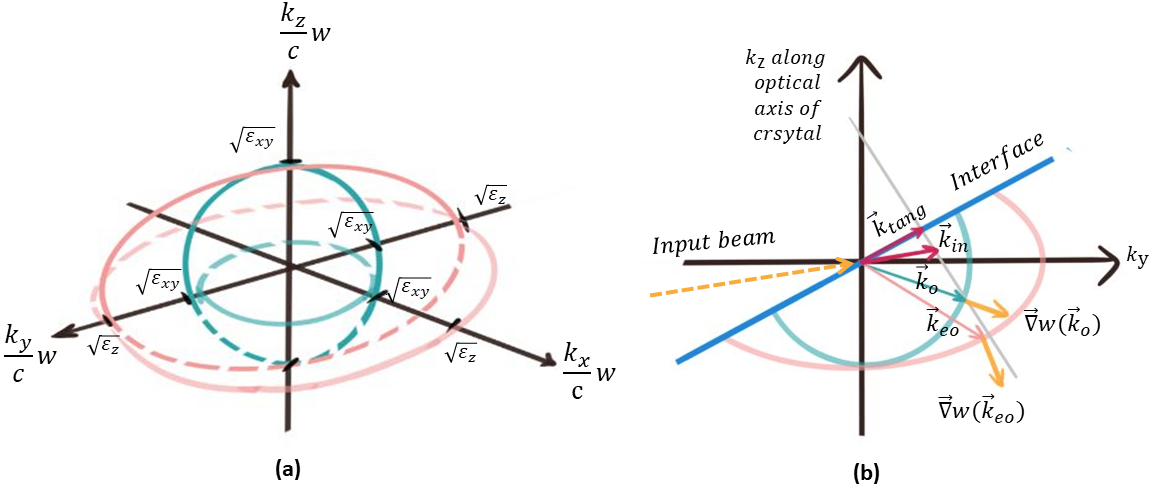
\includegraphics[width=0.82\linewidth]{uni.PNG}
    \caption{In (a) Fresnel's surface for a biaxial crystal is depicted following the text. In (b) for a plane wave $\vec{k}_{in}$ hitting an interface with a biaxial crystal in the dotted yellow line's direction, we see that if its tangential component $\vec{k}_{tang}$ must be preserved, two different $\vec{k}$, $\vec{k}_o$ and $\vec{k}_{eo}$ are allowed by the Fresnel surface. Then two beams will be refracted. Their propagation direction is given by the normals to the Fresnel surface $\vec{\nabla}w(\vec{k}_o)$ and $\vec{\nabla}w(\vec{k}_{eo})$, which are different (only the first one, the ordinary ray, follows Snell's law). }
        \label{fig:concentric1}
\vspace{-0.2cm}
\end{figure}

It was found in 1813 that there were some other crystals where birefringence was also present, but where there were two axes along which there was no double refraction. These were called {\bf biaxial crystals}, and are due to those lattices in which there is no clear symmetry axis: triclinic, monoclinic and rhombic systems, causing all the eigenvalues of $\pmb{\varepsilon}$ to be different. What was about to be discovered was that along these two axes there is no normal refraction either (as happens in the optical axis of uniaxial crystals). Instead, a conical refraction takes place.

In order to plot the Fresnel surface of a biaxial crystal, we can first obtain the shape of its intersections with the coordinate planes (which we choose to be aligned with the eigenvectors of $\pmb{\varepsilon}$). We will assume $\varepsilon_x<\varepsilon_y<\varepsilon_z$. If we check the surface at the $xy$ plane by setting $k_z=0$, we get $(k^2c^2-\varepsilon_zw^2)(c^2(\varepsilon_xk_x^2+\varepsilon_yk_y^2)-w^2\varepsilon_x\varepsilon_y)=0$, which are the circumference $k_x^2+k_y^2=\varepsilon_zw^2/c^2$ and the ellipse $\frac{k_x^2}{\varepsilon_y}+\frac{k_y^2}{\varepsilon_x}=w^2/c^2$. They do not intersect since $\varepsilon_z$ (the sphere radius) is the biggest eigenvalue of $\pmb{\varepsilon}$. The intersection with the $yz$ plane also gives a circumference and an ellipse that do not intersect (the circumference has a radius $\varepsilon_x$, the smallest eigenvalue). The intersection with the $xz$ plane on the other hand, gives an ellipse and a circumference that intersect in four points, because the circumference now has the intermediate radius $\varepsilon_y$ between the two semi-axes $\varepsilon_x$ and $\varepsilon_y$ of the ellipse. You can see this in Figure \ref{fig:concentric2}.a. For continuity and symmetry we can imagine the rest of the surface. It is a figure with four singular points where the two constant $w$ sheets touch. Two of them are along one same axis and the other two along another same axis, both in the plane $y=0$. Along these two axes, there is a single allowed phase velocity (single refractive index) for plane waves, else there are two. Finally, note how around each singular point each of the constant $w$ sheets forms a cone, the vertexes of which meet in the singular point, leaving the singular point in the center of a "diabolo"-like shape, as can be seen in the close-up of Figure \ref{fig:concentric2}.b. Thus the name diabolical singularity.\vspace{-0.15cm}

\begin{figure}[h!] 
\center
    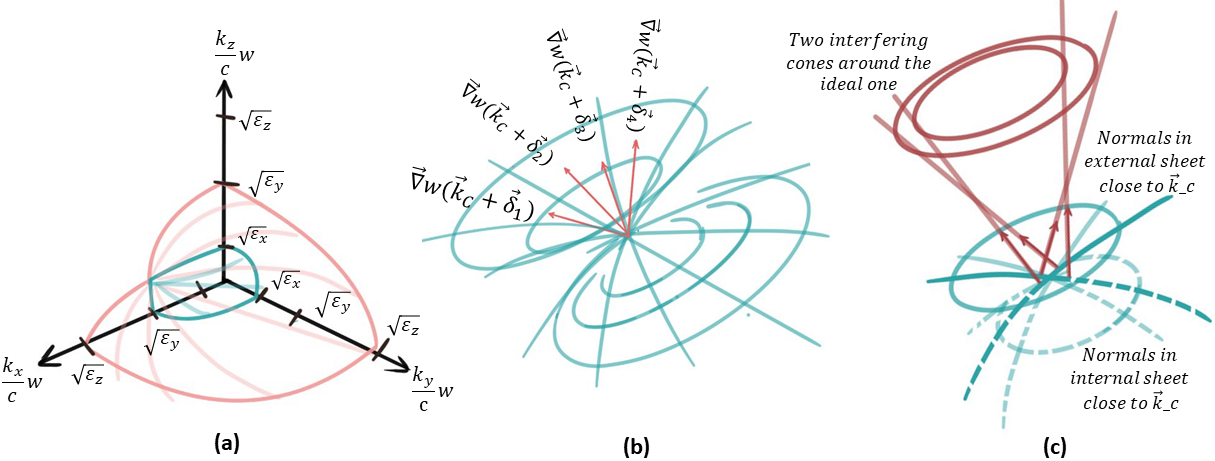
\includegraphics[width=0.95\linewidth]{bi.PNG}
    \caption{In (a) we see a plot of the first octant showing the intersections with the Fresnel surface of a biaxial crystal following the text. In (b) we see a depiction of a close-up of the diabolical singularity. Some normal vectors to the surface obtained by approaching to the singularity in different directions $\vec{\delta}_k$ in the surface, are shown. For $|\vec{\delta}_k|\rightarrow 0$, they form a cone of beams. In (c) we plot how the plane wave components close to the singularity (following the two sheets) refract generating two interfering cones that form a wide hollow ring. The ideal cone of Hamilton goes in between them.}
    \label{fig:concentric2}\vspace{-0.1cm}
\end{figure}

Now, we said that the normal to the constant $w$ surface indicated for a given wavevector, the propagation direction of a nearly monochromatic light ray with such a main plain wave in its decomposition. It turns out the tangent plane of the diabolical singularity is not well defined, neither its normal vector. However, since a real light ray, say a Gaussian laser beam, has other wavevector components around the wavevector matching the singularity, we can predict by continuity which will be the propagation direction for such a light ray. To do this, we will approach the singularity from one of the sheets. Note that the closer we get to the singularity, the closer will get the ensemble of the tangent planes to form a perfect cone, in the sense that the ensemble of normal vectors to these tangent planes around the singularity will each time be closer to a perfect conical bouquet of group velocities (see Figure \ref{fig:concentric2}.b). Thus, if a light beam enters a biaxial crystal cut orthogonally to one of its optical axes, and if the beam has its main wave-vector aligned with this optical axis, it will refract not as a single beam (as in typical refraction), nor as two beams (as in birefringence), but as a conical bouquet of "infinite" rays. Therefore, inside the crystal the light beam will open into a hollow cone of light. Once the cone of light arrives to the end face of the crystal, it will get out as a hollow ring of light. This is what Hamilton called {\bf Conical Refraction (CR)}. See a schematic picture in Figure \ref{fig:CR}.\vspace{0.2cm}

\mybox{{\bf The Relevance of Conical Refraction in the History of Physics}\vspace{0.2cm}\\
Back in the late 18-th century, a vivid battle was taking place in physics, between those who defended light was an ensemble of discrete corpuscles and those who defended it was a wave. The former had the authority of Sir Isaac Newton backing them \cite{newton}, while the latter really got momentum when Christiaan Huygens developed his theory of wavefronts \cite{huygens} in 1690, which allowed the description of birefringence for uniaxial crystals and how there was an axis along which this did not happen, a phenomenon that had no previous explanation. Yet, David Brewster found in 1813 that there were some crystals with two axes in which birefringence did not happen (biaxial crystals), which Huygens' theory could not explain. Moreover, Pierre Simon Laplace and Etienne Louis Malus achieved in 1809 the description of birefringence in terms of corpuscles \cite{laplace,malus}, so the battle was even. In 1801, Thomas Young revealed the light interference and slit diffraction phenomena \cite{young}, which were in favor of the wave nature of light. The big breakthrough though, happened in 1819, when Agustin-Jean Fresnel presented his wave theory of light \cite{fresnel}, by}
\mybox{which he was able to explain birefringence in both uniaxial and biaxial crystals together with interference and diffraction. For this he derived the equation we know today by his name just from geometrical intuitions (while we derived it from Maxwell's equations), when Maxwell was still about to be born. His theory was yet very involved and still the balance needed a further push to decide the winner posture.\\

This last push came from William Rowan Hamilton, who deeply studied Fresnel's surfaces and in 1832 found what we have seen \cite{hamilton}: the singularities of biaxial crystal surfaces were a double cone vertex, which meant a proper light beam crossing one of the optical axes of a biaxial crystal should refract as a cone and get out of the crystal as a hollow cylinder. A few weeks later, after being asked by Hamilton, Humphrey Lloyd was able to experimentally verify this fact \cite{lloyd}, making Hamilton's mathematical discovery, one of the {\bf first examples in the history of science where a mathematical prediction preceded its experimental discovery}. This was a hit in the struggle in favor of the wave description of light. Amazingly, after this, conical refraction remained as a pure curiosity and lost the interest of the community for about a century, with only sporadic contributions by scientists like Johann Christian Poggendorff (in 1839) \cite{poggendorff} or Chandrasekhara Venkata Raman (in 1941) \cite{raman1,raman2} among others, who discovered that in fact the ring was split in two light rings by a dark ring, known today as the Poggendorff dark ring, or the fact that focusing the beam, it was in the focal plane where the ring was most clearly visible, such that away from it, the ring contracts until a light point, achieving a maximum axial intensity in which today is known as the Raman spot.\\ 

The disappearance of CR was in part because a full diffraction theory was to be developed in order to account for the complexity of the phenomenon, and in part because the experimental fineness for a decent account of its verification would only be achievable in the last half of the 20-th century, with the advance of laser and crystal engineering technologies \cite{Todor}. It was in this last period of the century that a revival of the interest in CR emerged, when the complete mathematical formulation for the phenomenon \cite{BK1, BK2, Berry, Jeffrey} (as we will review in a moment) and uncountable applications for it \cite{Turpin} (among others the polarimeter developed in this thesis) were suggested \cite{Stokes1, Stokes2, incomplete}.
}

There is one last consideration. Voigt discovered in 1905 \cite{voigt, Jeffrey} that the intensity of light refracted along a normal to a general Fresnel's surface was proportional to the area element of the surface around the (main) wave-vector of the given beam. This can be understood qualitatively, because a real light beam is also composed of a continuous range of wave-vectors around the central one, which means when we consider the refraction law (taking the tangent component of $\vec{k}_{in}$ to the interface), we are really considering a continous patch of tangent components, which translate into an area element in the intersections with Fresnel's surface. Following this, Voigt realized that since in the diabolo singularity of a biaxial crystal, the area element is null, the ideal cone of Hamilton should have no intensity. This would imply, that the generated hollow ring has only light for the $\vec{k}$ components close to the singularity, but not for the singularity $\vec{k}$; meaning the ring should be split in two rings by a dark ring corresponding to Hamilton's ideal cone (see Figure \ref{fig:concentric2}.c). Indeed, as was experimentally found by Poggendorff, this is the case. We call it the {\bf Poggendorff dark ring}.

With all this, the conical refraction phenomenon is qualitatively (and quite quantitatively as we will see) determined by three parameters. The first one is the {\bf semi-angle} of the cone $\alpha$, which can be geometrically proven using Fresnel's surface to be $\alpha=\sqrt{(\varepsilon_y-\varepsilon_x)(\varepsilon_z-\varepsilon_y)/\varepsilon_y}$ for $\varepsilon_x<\varepsilon_y<\varepsilon_z$. Then, given the length of the biaxial crystal slab $L$ along the optical axis, we can get the {\bf geometric radius} of the hollow ring to be $R_0=L\;tan(\alpha)$. It can be proven geometrically that the cone is slanted such that it opens in the plane of the two optical axes, as shown in Figure \ref{fig:CR}. Finally, since our input beam will have a Gaussian profile in the transversal section to the propagation, we need to define its width, which we call the {\bf beam waist} $w_0$. This parameter will determine how many plane wave components around the singularity compose the input beam, and thus will be proportional to the width of the generated hollow ring. A Gaussian beam will naturally tend to open if we leave it free (for its plane-wave components cannot be parallel). Thus, a unique definition of the beam waist $w_0$ can be given if for example, we focus the Gaussian beam and define $w_0$ to be the full width at half maximum (divided by $\sqrt{2log(2)}$) at the focal plane, where the beam will get most concentrated.

\begin{figure}[h!] 
     \centering 
         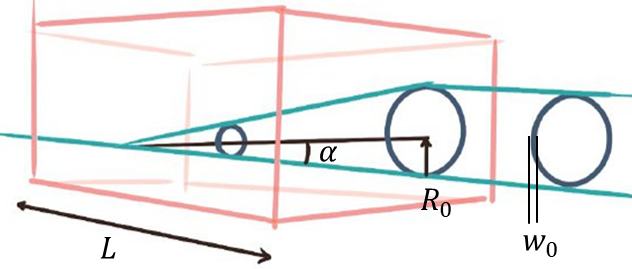
\includegraphics[width=0.5\linewidth]{cr.PNG}
    \caption{Schematic depiction of the classical description of conical refraction, with its main parameters.}
    \label{fig:CR}
\end{figure}
Before we continue, it is important to note that it turns out the most defined picture of the ring is generated only at infinity (far away from the entry point), which is the reason why a focusing lens will be used before the beam enters to the crystal: it will take the image formed at infinity to the focal plane, which is at a finite distance.

%$(k^2c^2/w^2-\varepsilon_{xy})\qty(c^2/w^2(\varepsilon_zk_z^2+\varepsilon_{xy}(k_x^2+k_y^2))-\varepsilon_z\varepsilon_{xy})=0$ 

\section*{A.2. The Belskii-Khapalyuk-Berry Description of the Phenomenon }
\addcontentsline{toc}{subsection}{2. The Belsky-Khapalyuk-Berry Description of the Phenomenon }
\fancyhead[OR]{The Belsky-Khapalyuk-Berry Theory }
\fancyhead[EL]{The Belsky-Khapalyuk-Berry Theory }

So far we have understood when the phenomenon happens and which is the shape of the overal light beam. Yet, we have not seen what happens with the state of polarization, which will be the key to develop the polarimeter. To understand this and to be able to simulate the phenomenon, we will need to introduce part of the full diffractive theory in biaxial crystals developed by Belskii and Khapalyuk in 1978 \cite{BK1,BK2}, and reformulated by Michael V. Berry in 2004 \cite{Berry}. We will proceed to present the cylindrically symmetric solution, as presented by Alex Turpin in Ref. \cite{Turpin}.\vspace{-0.1cm}

Let us consider a biaxial crystal with mean refractive index $n$ and one of its optical axes aligned with the $z$ Cartesian coordinate axis. Before the crystal a focusing lens will be placed as explained above, so we will consider the $z$ coordinate is centered in the focal plane. In addition, we will consider the coordinates $x,y$ are in waist radius $w_0$ units, while $z$ is in Rayleigh length units $z_R:=\pi w_0^2n/\lambda$, being $\lambda$ the main wavelength of the input beam. Finally, we will consider an input light beam $\vec{D}_0(\vec{r}\,)$ with its spatial Fourier decomposition in plane waves, such that all the expansion weights are centered around one $\vec{k}$ with a particular $k_z$ directed in the $z$ axis, $k_z>0$. We will assume that for all significant $\vec{k}$ in its decomposition, $k_z>>k_x,k_y$. This is called the paraxial approximation. It implies, as we saw, not only that the displacement field will have null component in $z$, but also that the other two components will vary sinusoidally in the $z$ direction, allowing us to center our attention in the distribution of the electric field only in the transversal plane $z=0$, $\vec{D}(\vec{q};z)=(D_x(\vec{q};z),D_y(\vec{q};z), 0)$ with $\vec{q}:=(x,y)$. In addition we will assume that after passing through a medium, the light beam is describable with its displacement vector $\vec{D}$ (for the effect of bound charges will become negligible).

The approach followed in the Belskii-Kahapalyuk-Berry (BKB) formulation is to first derive the effect that the biaxial crystal has on a particular plane wave with transversal wavenumber $\vec{k}=(k_x,k_y)$ (the dominant $k_z$ component is presumed). Then if we decompose the input wave in its transversal Fourier spectrum and apply the effect to each plane wave component, by the linearity of Maxwell's equations, we will get the evolution of the entire wave. Remember that what gave the CR ring its pattern were actually the plane wave components that were close but not equal to the singularity $\vec{k}$ exactly aligned with the optical axis, for which $k_x,k_y=0$. This fact is here made explicit when considering the distribution of all the rest of components.

Berry proves in \cite{Berry, BerryJeffrey} that a lowly birefringent biaxial crystal causes a unitary transformation $\pmb{U}(\vec{k})=e^{-i\pmb{\Gamma}(\vec{k})}$ to an input plane wave $\vec{k}$ close to the singularity, such that $\pmb{\Gamma}$ is the Hermitian operator $\pmb{\Gamma}(\vec{k}):=\frac{1}{2}|\vec{k}|^2z^2\pmb{Id}+\rho_0\vec{k}\cdot (\pmb{\sigma_z}, \pmb{\sigma_x})$. Here, $\pmb{\sigma_z}, \pmb{\sigma_x}$ denote the $x$ and $z$ Pauli matrices and we define $\rho_0\equiv R_0/w_0$ to be the geometric radius of the CR ring in waist radius units (or the ratio between the geometric radius of the ring and the waist radius of the beam). Then, by considering the identity $e^{i\vec{v}(\vec{n}\cdot \vec{\sigma})}=\pmb{Id}cos(v)+i(\vec{n}\cdot \vec{\sigma}) sin(v)$ given a vector $\vec{v}=v\vec{n}$ with $|\vec{n}|=1$ and given $\vec{\sigma}=(\pmb{\sigma_x},\pmb{\sigma_y},\pmb{\sigma_z})$ is the vector of Pauli matrices, we can rewrite the unitary as:\vspace{-0.1cm}
\begin{equation}
\pmb{U}(\vec{k}) = e^{-i\frac{1}{2n}|\vec{k}|^2z^2}\qty[cos\qty(\rho_0|\vec{k}|)\pmb{Id}+i\;sin\qty(\rho_0|\vec{k}|)\frac{\vec{k}}{|\vec{k}|}\cdot (\pmb{\sigma_z},\pmb{\sigma_x})]\vspace{-0.1cm}
\end{equation}
Given the transversal Fourier transform of the input beam $\vec{D}_0(\vec{q}\,)=(D_{0x}(\vec{q}\,), D_{0y}(\vec{q}\,)\,)$ in $\vec{k}=(k_x,k_y)$:
\begin{equation}
A_x(\vec{k}):=\frac{1}{(2\pi)^2}\iint_{\R^2} D_{0x}(\vec{q}\,)e^{-i\vec{k}\cdot\vec{r}}dx\;dy \quad \quad \quad A_y(\vec{k}):=\frac{1}{(2\pi)^2}\iint_{\R^2} D_{0y}(\vec{q}\,)e^{-i\vec{k}\cdot\vec{r}}dx\;dy
\end{equation}
We can obtain the post-crystal displacement vector field (remember it has only component in $x,y$) by applying the unitary transformation to the plane wave coefficients of the input beam $\vec{A}(\vec{k})$ and then taking the result back to position space:
\begin{equation}
\vec{D}(\vec{q};z)=\frac{1}{(2\pi)^2}\iint_{\R^2}e^{i\vec{k}\cdot\vec{q}}\;\pmb{U}(\vec{k})\vec{A}(\vec{k})dk_xdk_y
\end{equation}
This can be expanded to a simpler form in cylindrical coordinates $\vec{k}=k(cos(\phi_k),sin(\phi_k))$, $\vec{q}=q(cos(\varphi), sin(\varphi))/w_0$ with $\phi_k,\varphi\in[-\pi,\pi)$ and $q,k>0$ as:
\begin{equation}\label{geez}
\vec{D}(q,\varphi;z)=\frac{1}{(2\pi)^2}\int_{-\pi}^{\pi}\int_{0}^\infty e^{ikq \;cos(\phi_k-\varphi)}e^{-i\frac{1}{2n}k^2z^2}\begin{pmatrix}
cos(\phi_k) & sin(\phi_k)\\
sin(\phi_k) & -cos(\phi_k)
\end{pmatrix} \vec{A}(\vec{k})\;k\;dk\;d\phi_k
\end{equation}
We now consider that the input beam is cylindrically symmetric with a uniform polarization $\vec{E}(\vec{q}\,)=E(q)\hat{u}_J$, with $\hat{u}_J$ its Jones vector. Its Fourier transform will also be cylindrically symmetric, such that $A_x(\vec{k})=A_y(\vec{k})=a(k):=\int_0^\infty E(q)J_0(qk)k dr$, where $J_n(x)$ is the $n^{th}$ order Bessel function of the first type. This assumption then allows integrating equation \eqref{geez}
over $\phi_k$, using the Bessel function identities: $\int_{-\pi}^{\pi}e^{ik\rho\;cos(\phi_k-\varphi)}d\phi_k=J_0(k\rho)$ and $\int_{-\pi}^{\pi}e^{ik\rho\;cos(\phi_k-\varphi)}cos(\phi_k)d\phi_k=cos(\varphi)J_1(k\rho)$. This leaves the computation of $\vec{D}$ as a one dimensional integral:\vspace{0.1cm}
\begin{equation}\label{master}
\vec{D}(q, \varphi;z)=\begin{pmatrix}
B_0(q;z)+B_1(q;z)cos\varphi & B_1(q;z) sin\varphi\\
B_1(q;z)sin\varphi & B_0(q;z)-B_1(q;z)cos\varphi
\end{pmatrix}\hat{u}_J\vspace{0.1cm}
\end{equation}
where $B_0,B_1$ are known as the BKB integrals, which note that only depend on $q,z$:
\begin{equation}\label{bkb1}
B_0(q;z)=\frac{1}{2\pi}\int_0^\infty a(k)e^{-i\frac{k^2z^2}{2n}}cos(k\rho_0)J_0(kq)k\;dk
\end{equation}
\begin{equation}\label{bkb2}
B_1(q;z)=\frac{1}{2\pi}\int_0^\infty a(k)e^{-i\frac{k^2z^2}{2n}}sin(k\rho_0)J_1(kq)k\;dk
\end{equation}
Finally, we can get the intensity pattern of light $I(q,\varphi;z)$, by taking the magnitude squared of $\vec{D}$ (its real part). This intensity pattern in $q,\varphi$ for a fixed $z$ is what we expect to be captured by a camera (or our eye) if the sensor is placed orthogonal to the optical axis at a distance $z$ from the focal plane.

\subsubsection*{A.2.1. The angular shape of the emerging pattern depends on the input polarization}

We can now predict what we will see/capture as a function of the polarization of the input beam. If we evaluate in equation \eqref{master} the Jones vector for circular polarization (CP), $\vec{u}_J=\frac{1}{\sqrt{2}}(1,\pm i)$ (a quarter period relative phase $e^{i\pi/2}=i$), we can easily arrive at:
\begin{equation}
I_{CP}(q,\varphi;z)=|\mathfrak{R}e\{\vec{D}(q,\varphi;z)\}|^2=|B_0(q;z)|^2+|B_1(q;z)|^2
\end{equation}
Since $B_0,B_1$ do not depend on $\varphi$, we see that the intensity pattern for CP only depends radially on $q$, $I_{CP}(q,\varphi;z)=I_{CP}(q;z)$. This implies that the intensity pattern is symmetric in its angular component. That is, if we take the integral in $q$ for the intensity pattern:\vspace{-0.1cm}
\begin{equation}\label{yoyo}
\mathcal{I}_{CP}(\varphi;z)=\int_0^\infty I_{CP}(q,\varphi;z)q\;dq=C(z)
\end{equation}
we get a same value $C$ for all $\varphi$ (for a fixed $z$).\footnote{We have assumed the total transversal intensity $\int_0^\infty \int_{-\pi}^{\pi}I_{CP}(q,\varphi;z)d\varphi\;qdq=\int_0^\infty2\pi\qty(|B_0(q;z)|^2+|B_1(q;z)|^2)q\;dq$ (which is the $L_2$ norm for the electric field) converges to a real number, which is to be expected since a physical input wave's transversal intensity pattern will always have a total finite intensity or "norm" (for example the Gaussian profile given next in \eqref{Four} has a finite integral in $q$). Then, following Parseval's identity, its integral (norm) in Fourier space will also be finite, meaning that since the unitary transformation $\pmb{U}$ of the crystal will preserve its norm, by reverting the Fourier transform to get $\vec{D}$ we would still have the same finite norm or total intensity for each transversal section.  } This is in accordance with out intuition that a hollow ring should be generated.\vspace{-0.1cm}

If instead we evaluate the Jones vector for an arbitrary linear polarization (LP) at an angle $\Phi_{LP}$ with the $x$ axis, say $\vec{u}_J=(cos\Phi_{LP}, sin\Phi_{LP})$, after several trigonometric identities and some hard work, we can arrive to:\vspace{-0.1cm}
\begin{equation}\label{Pre}
I_{\Phi_{LP}}(q,\varphi;z)=I_{CP}(q;z)+2\mathfrak{R}e\qty{B_0(q;z)B_1^*(q;z)}cos(2\Phi_{LP}-\varphi)
\end{equation}
where $b^*$ denotes complex conjugation of $b\in\C$. We can derive an important result here. Following Berry and Jeffrey \cite{Berry, BerryJeffrey, Jeffrey}, since we are interested in thick crystal slabs and ligth beams with small waist, such that $R_0>>w_0$, around $z=0$, we can plug asymptotic expressions for the Bessel functions in $B_0,B_1$ for we consider large enough $q$. Up to oscillatory terms that become negligible when integrated, we can then consider:\vspace{-0.1cm}
\begin{equation}
cos(k\rho_0)J_0(kq)\simeq sin(k\rho_0)J_1(kq)
\end{equation}
This makes $B_0(q;0)\simeq B_1(q;0)$ for the significant values on the ring, yielding for the linear polarization intensity \eqref{Pre}, (by using $1+cos(x)=2cos^2(x/2)$): $I_{\Phi_{LP}}(q,\varphi;z)=2|B_0(q;0)|^2cos^2(\varphi/2-\Phi_{LP})$. The angular pattern will then be:
\begin{equation}\label{cosine}
\mathcal{I}_{\Phi_{LP}}(\varphi;z)=C(z)cos^2(\frac{\varphi}{2}-\Phi_{LP})
\end{equation}
This means that if we input a light beam with a linear polarization at an angle $\Phi_{LP}$ with the $x$ axis, the image at the focal plane will have an angular pattern with a single peak in $\Phi_{LP}$ and a single valley in its diametrically opposed angle, while the intensity will continuously change in between. This suggests that for an input LP light, the CR ring will not be complete. Instead a sort of "croissant" or crescent moon shape is suggested to be shaped. A moon with its maximum pointing in the direction indicating the angle $\Phi_{LP}$ at which the LP light was polarized. This readily suggests the device we wish to design.
\vspace{-0.1cm}


\section*{A.3. Simulating the Phenomenon \vspace{-0.1cm} }
\addcontentsline{toc}{subsection}{3. Simulating the Phenomenon }
\fancyhead[OR]{Simulating the Phenomenon }
\fancyhead[EL]{Simulating the Phenomenon }
Assuming we use a focused input laser beam directed along one of the optical axes of a biaxial crystal, such that in its focal plane it has a beam waist of $w_0$ in the absence of the crystal, we saw that equation \eqref{master} will yield the resulting electric field of the light at a distance $z$ from the focal plane.    We can generate theoretical images that a camera placed along $z$ should register by computing first the BKB integrals \eqref{bkb1},\eqref{bkb2} numerically and then computing the whole field $\vec{D}(q,\varphi,z)$ and the intensity pattern $I(q,\varphi,z)=|\vec{D}(q,\varphi,z)|^2$  for a desired input polarization $\hat{u}_J$ with \eqref{master}.

Since experimentally we can easily obtain a laser beam with a Gaussian transversal profile, we consider from now on that the input beam is so:\vspace{-0.15cm}
\begin{equation}\label{Four}
\vec{D}_0(\vec{q}\,)=D_0e^{\frac{-q^2}{2}}\hat{u}_J \quad \quad a(k)=a_0e^{-k^2/2}
\end{equation}
for some real constants $D_0,a_0$.

With all the given, the resulting theoretical images were simulated as follows:
\begin{enumerate}
\item Let the user choose the average refractive index $n$, the parameters $w_0,R_0,z$ in pixel units (where each pixel is then in our normalized units) and fix $\hat{u}_J$ for the polarization of the input wave.
\item Generate a numerical Cartesian grid emulating the pixel grid of the photographic camera. Obtain the polar coordinates of each pixel of the grid. 
\item Choose the maximum $k$ until where we will integrate and how many points to consider within this line. It is important to take the biggest and densest possible range.
\item For each considered radial distance $q$ in the image plane, compute the BKB integrals \eqref{bkb1},\eqref{bkb2} using a composite trapezoidal rule. For this, first numerically compute the Bessel functions over the $k$ points for the given $q$ and with them compute the whole integrand at each $k$ point and $q$. Finally, add all the $k$ integrand evaluations for each fixed $q$ multiplied by the $k$ step. This should be done in a vectorized and optimized way, for it is the bottleneck of the simulation.
\item Compute the displacement field at each pixel of the image $\vec{D}$, using the matrix equation \eqref{master} with the input Jones vector and the computed BKB integrals at each pixel.
\item Compute the intensity at each pixel location with the squared norm of the real part of $\vec{D}$. This will be what a camera at $z$ should see.\vspace{-0.2cm}
\end{enumerate}

This simulator was implemented in Python in two versions, first as a sequential vectorized calculator using the {\em numpy} library 	\cite{numpy} and then as a batched GPU parallelized version employing both {\em jax} \cite{jax} and {\em pytorch} \cite{pytorch}. These can be found in the Github repository \cite{github} with the rest of the generated code and material. 

We now proceed to show some simulated results that will allow us understand more deeply the phenomenon of CR. Essentially, the generated profile has four degrees of freedom in our study: $R_0,w_0,z$ and the input polarization $\hat{u}_J$. Lets see their effect.\vspace{-0.2cm}



\subsubsection*{Observation 1: The cone has a spatial polarization-dependent intensity distribution}
We can see in Figure \ref{fig:simul1}.a, for a given fixed $R_0,w_0$ that input CP light generates a hollow uniform ring in the focal plane $z=0$, just as predicted in (A.2.1). However, if instead we input a LP light, as we do in Figure \ref{fig:simul1}.b, with say, an electric field oscillating at a fixed $\pi/2$ rad plane relative to the $x$ axis\footnote{We will assume all angles are relative to the $x$ axis of the camera from now on.} (oscillating along the vertical), we note that the ring lacks an intensity point and has a maximum intensity spot diametrically opposed to it. Indeed this is what we predicted would happen in (A.2.1). 

To better illustrate this point, now that we have full information of the electric field, we can analyze which is the polarization of light at each point along the ring. As depicted in Figure \ref{fig:simul2}, it turns out that along the ring light is found to be linearly polarized, no matter if we inputted LP or CP. Not only that, but the LP angle in each point of the ring is fixed with the crystal. Then, if we choose to input a beam with an electric field that has zero projection into a certain direction, it turns out that (a) there is no light in the point of the ring where that component should be placed, while (b) there is maximum intensity where the LP matching the input beam's angle appears. When we input circular or randomly polarized light into the crystal, every point in the ring has light, because it is a beam that has a non-zero projection component into any orthogonal pair of axes that we could choose in the transversal profile. In fact, since this decomposition has an equal magnitude in all pair of axes, the ring appears to have an homogeneous intensity. These two findings correspond with the predictions we obtained in section (A.2.1) about the angular intensity pattern. Not only that, but in accordance with what we found there, we can verify in Figure \ref{fig:simul1} that {\bf the intensity of light is distributed along the ring in a cosinusoidal fashion for input LP, while it is constant in CP}. All this suggests that the crystal acts as an continuous set of different linear polarizers spatially splitting the input beam.

The most important thing here is that given the input light is linearly polarized, {\bf with a single image of the intensity getting out of the crystal, we are able to know the LP by looking at the maximum and minimum spots}.


\begin{figure}[h!] 
     \centering 
    \begin{subfigure}[b]{0.24\linewidth}
    
\includegraphics[width=\linewidth]{simul11.png}
    \caption{CP }
     \end{subfigure}
 \begin{subfigure}[b]{0.25\linewidth}
     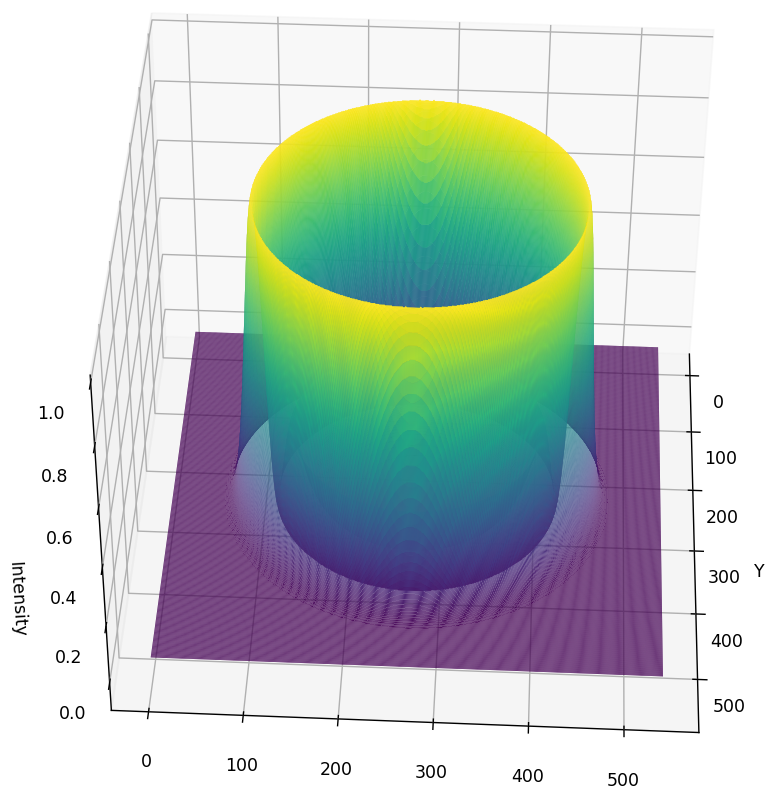
\includegraphics[width=\linewidth]{simul12.png}
    \caption{CP }
     \end{subfigure}
 \begin{subfigure}[b]{0.24\linewidth}
     
\includegraphics[width=\linewidth]{simul13.png}
     \caption{LP}
     \end{subfigure}
  \begin{subfigure}[b]{0.25\linewidth}
     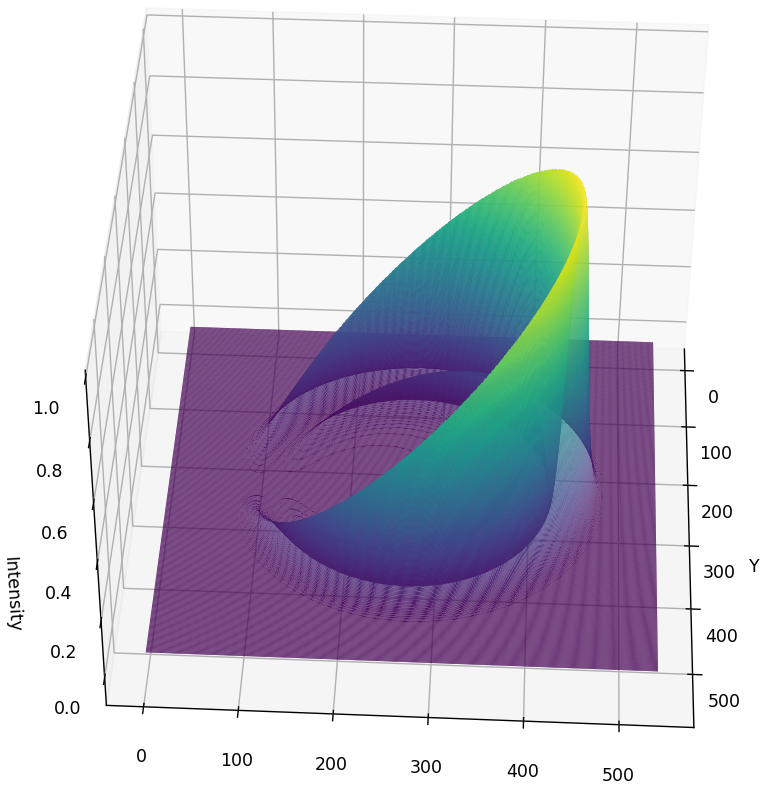
\includegraphics[width=\linewidth]{simul14.png}
     \caption{LP }
     \end{subfigure}
    \caption{Simulated CR rings at $z=0$, $R_0=167$ pix, $w_0=24$ pix for input CP in (a),(b) $\hat{u}_J=\frac{1}{\sqrt{2}}(1,i)$ and LP in (c),(d) $\hat{u}_J=(1,0)$. (a),(c) represent the simulated intensity $|\vec{D}|^2$ as a grayscale heatmap, while (b),(d) show it as a surface plot.}
        \label{fig:simul1}
\end{figure}

\begin{figure}[h!] 
     \centering 
    \begin{subfigure}[b]{0.245\linewidth}
    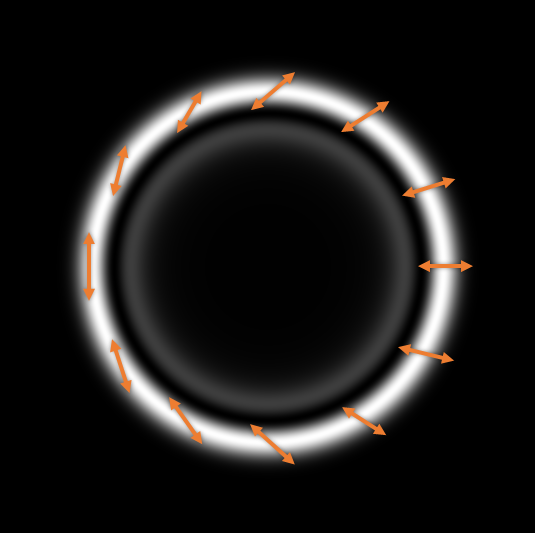
\includegraphics[width=\linewidth]{simul21.PNG}
    \caption{CP }
     \end{subfigure}
 \begin{subfigure}[b]{0.245\linewidth}
     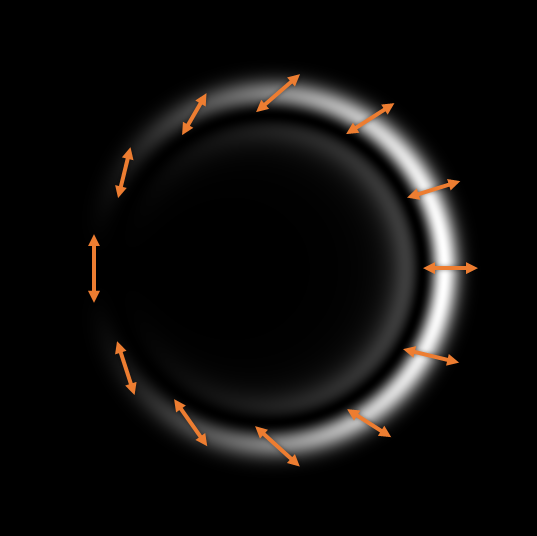
\includegraphics[width=\linewidth]{simul23.PNG}
    \caption{LP 0 rad}
     \end{subfigure}
 \begin{subfigure}[b]{0.245\linewidth}
     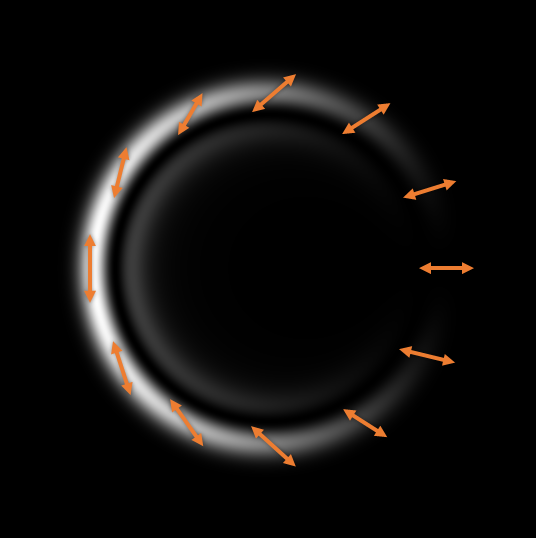
\includegraphics[width=\linewidth]{simul22.PNG}
     \caption{LP $\pi/2$ rad}
     \end{subfigure}
  \begin{subfigure}[b]{0.245\linewidth}
     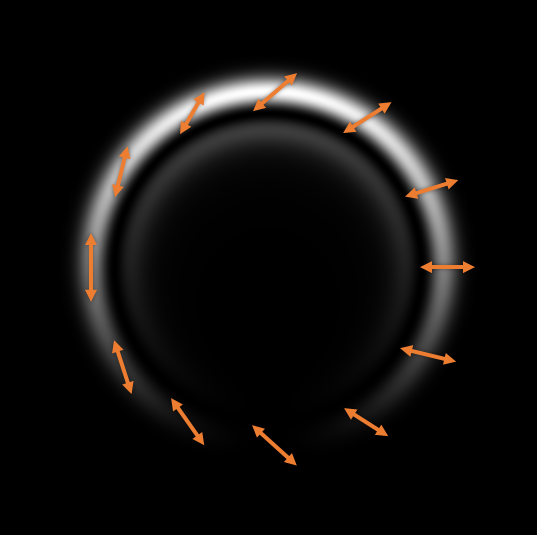
\includegraphics[width=\linewidth]{simul24.PNG}
     \caption{LP $\pi/4$ rad}
     \end{subfigure}
    \caption{Simulated CR rings at $z=0$, $R_0=167$ pix, $w_0=24$ pix. Input CP in (a) $\hat{u}_J=\frac{1}{\sqrt{2}}(1,i)$ and LP in (b),(c),(d) $\hat{u}_J=(cos(\Phi_{LP}),sin(\Phi_{LP}))$ with $\Phi_{LP}=0,\pi/2,-\pi/4$ respectively. The normalized intensity is shown as a grayscale heatmap. The arrows indicate the direction of oscillation of $\vec{D}$ in the spatial point below them.}
            \label{fig:simul2}

\end{figure}

\subsubsection*{Observation 2: The $w_0,R_0$ trade-off}
We can clearly see in any of the figures of this section, the dark Poggendorff ring separating the light into two rings. It is on this dark ring where Hamilton's ideal cone should be placed as we described previously. Thus, this is the ring that will define the geometrical radious $R_0$. 

If we then modify $R_0,w_0$ such that the ratio $\rho_0=R_0/w_0$ is preserved, we can see that the image we get is the same but zoomed in or out (see Figure \ref{fig:simul3}). By fixing a certain $R_0$, we can see in Figure \ref{fig:simul4} how the ring changes if we modify $\rho_0$. If $\rho_0$ is made too small, the clear segregation of the linear polarizations starts to get more diffuse. Yet, if $\rho_0$ is too big, the ring gets very slim, which means that less pixels of the image will carry information about the ring (thus if the camera has some error per pixel, the information will get more diffuse). Then the best thing would be to {\bf choose an $R_0$ that occupies most of the camera sensor (most pixels), without getting out of the camera plane, and by playing with $w_0$, choose the most convenient $\rho_0$ in the stated trade-off}.

Experimentally the problem will be that since $R_0$ is fixed by the employed crystals' length, refractive indices and the camera's pixel density, we will only have the chance to modify $w_0$, which is not as helpful in trying to spread the intensity pattern through the entire camera sensor. It is this why we will employ magnifying lenses after the crystal and before the camera to make the ring of the focal point physically bigger (without altering the $\rho_0$ parameter), virtually just as done in Figure \ref{fig:simul3}.
\begin{figure}[h!] 
     \centering 
    \begin{subfigure}[b]{0.245\linewidth}
    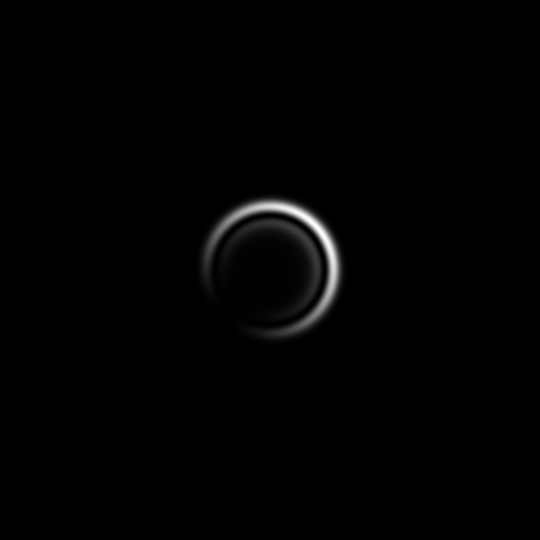
\includegraphics[width=\linewidth]{simul31.png}
    \caption{$\rho_0=6$\\ $w_0=10$ $R_0=60$}
     \end{subfigure}
 \begin{subfigure}[b]{0.245\linewidth}
     
\includegraphics[width=\linewidth]{simul32.png}
    \caption{$\rho_0=6$\\ $w_0=20$ $R_0=120$}
     \end{subfigure}
 \begin{subfigure}[b]{0.245\linewidth}
     
\includegraphics[width=\linewidth]{simul33.png}
    \caption{$\rho_0=6$\\ $w_0=30$ $R_0=180$}
     \end{subfigure}
  \begin{subfigure}[b]{0.245\linewidth}
     
\includegraphics[width=\linewidth]{simul34.png}
    \caption{$\rho_0=6$\\ $w_0=36$ $R_0=220$}
     \end{subfigure}
    \caption{Simulated CR rings at $z=0$ for input LP $\hat{u}_J=\frac{1}{\sqrt{2}}(1,1)$ and varying $R_0, w_0$ while $\rho_0=R_0/w_0$ remains fixed. The normalized intensity is shown as a grayscale heatmap.}
            \label{fig:simul3}
\end{figure}

\begin{figure}[h!] 
     \centering 
    \begin{subfigure}[b]{0.245\linewidth}
    
\includegraphics[width=\linewidth]{simul41.png}
    \caption{$\rho_0=2$\\ $w_0=83.5$ $R_0=167$}
     \end{subfigure}
 \begin{subfigure}[b]{0.245\linewidth}
     
\includegraphics[width=\linewidth]{simul42.png}
    \caption{$\rho_0=4$\\ $w_0=41.75$ $R_0=167$}
     \end{subfigure}
 \begin{subfigure}[b]{0.245\linewidth}
     
\includegraphics[width=\linewidth]{simul43.png}
    \caption{$\rho_0=8$\\ $w_0=20.87$ $R_0=167$}
     \end{subfigure}
  \begin{subfigure}[b]{0.245\linewidth}
     
\includegraphics[width=\linewidth]{simul44.png}
    \caption{$\rho_0=16$\\ $w_0=10.44$ $R_0=167$}
     \end{subfigure}
    \caption{Simulated CR rings at $z=0$ for input LP $\hat{u}_J=\frac{1}{\sqrt{2}}(1,1)$ for varying $\rho_0$. The normalized intensity is shown as a grayscale heatmap.}
            \label{fig:simul4}
\end{figure}


\subsubsection*{Observation 3: Going out of the focal plane the ring is lost}
In Figure \ref{fig:simul5}, we vary where the camera is placed relative to the focal plane $z=0$. Clearly, {\bf the rings and their intensity distribution are most clearly visible in the focal plane} (which would represent the infinity for the crystal). Going out of $z=0$ we loose the structure until at $z=\pm\sqrt{4/3}\rho_0$, known as the Raman spots, we just find a spike that barely gives us information.

\begin{figure}[h!] 
     \centering 
    \begin{subfigure}[b]{0.245\linewidth}
    
\includegraphics[width=\linewidth]{simul599.png}
    \caption{$z=\pm3$}
     \end{subfigure}
 \begin{subfigure}[b]{0.245\linewidth}
     
\includegraphics[width=\linewidth]{simul5990.png}
    \caption{$z=\pm1.8$}
     \end{subfigure}
 \begin{subfigure}[b]{0.245\linewidth}
     
\includegraphics[width=\linewidth]{simul5999.png}
    \caption{$z=\pm1.5$}
     \end{subfigure}
  \begin{subfigure}[b]{0.245\linewidth}
     
\includegraphics[width=\linewidth]{simul59990.png}
    \caption{$z=\pm1.2$}
     \end{subfigure}
    \caption{Simulated CR rings with fixed $R_0=167$, $w_0=24$ and input CP $\hat{u}_J=\frac{1}{\sqrt{2}}(1,\pm i)$. Varying $z$. The corresponding one to $z=0$ is Figure \ref{fig:simul1}.a. The normalized intensity is shown as grayscale heatmap. If the input light is linearly polarized, the resulting images are the same but are angularly modulated by a cosine square (just as in $z=0$).}
            \label{fig:simul5}
\end{figure}
\section*{A.4. A Natural Polarimeter}
\addcontentsline{toc}{subsection}{4. A Natural Polarimeter }
\fancyhead[OR]{A Natural Polarimeter }
\fancyhead[EL]{A Natural Polarimeter }
The reader will have understood by now the idea that will be behind the device to measure the linear polarization of light. The CR phenomenon naturally acts as if in each point of the generated hollow ring there was a differently oriented linear polarizer, such that in a single camera image we can have the result of passing the input light beam from all the possible linear polarizers (if the resolution of the camera was infinite, of course). As a consequence, given an unknown input LP light beam, we will be able to know the angle at which the input field is oriented by looking at where the angular maximum (or minimum) intensity spot is placed. If we can process each photo fast enough, we could then measure in real time how the plane of an input LP light changes. Once this idea is in the table (as suggested already by for instance Refs. \cite{Stokes1, Stokes2, incomplete}), the main mystery to be solved would be the computer vision problem of getting the angle at which the crescent ring is oriented.

In principle this would seem to be limited to LP measurements. Yet, by dividing the input beam into two (by means of partial mirrors for example), and by employing two biaxial crystals, it is possible to build a full polarimeter that also gives all the ellipticity information. This was shown by Refs. \cite{Stokes1, Stokes2}. One of the arms of this device should place a quarter wave-plate before the crystal, which then using the Mueller matrices would let us know the missing polarization information.

However, following the line of reference \cite{incomplete} this implies complicating the design of the device, requiring double elements, from crystals to cameras, with the complication of their synchronization. Not only that, but the cost of the device would double. It turns out, for numerous interesting applications, the measurement of LP is enough.\footnote{In any case, the computational solutions given in this thesis are still equally applicable to such a complete polarimeter.} Let us now illustrate the importance of LP measurements with several examples. 
\begin{itemize}

\item{\bf Example in Pharmacology: }There are chemical compounds (most organic compounds) that can have exactly the same elements and bonds between them and even still have two possible molecules. Just the same way as our two hands have the "same" composing bones and unions between bones, and yet they are not identical. They are mirror images. In chemistry this is called optical isomerism or enantiomerism. For example, the two molecules in Figure \ref{fig:thalidomide} are the same compound, with identical chemical and physical properties, except for the fact that a dissolution of one rotates the plane of polarization of an input LP light in one direction, while the other one rotates exactly the same amount in the other direction. If we have a mixture of them, where they are in equal proportions, the net LP of light does not change when crossing the dissolution. Thus, if we measure the amount of rotation of the plane of polarization, we can know the exact proportion of these enantiomers present in the mixture \cite{enantiomers}. It turns out this is the only trivial way to measure the presence and proportion of enantiomers. 

\begin{figure}[h!] 
     \centering 
    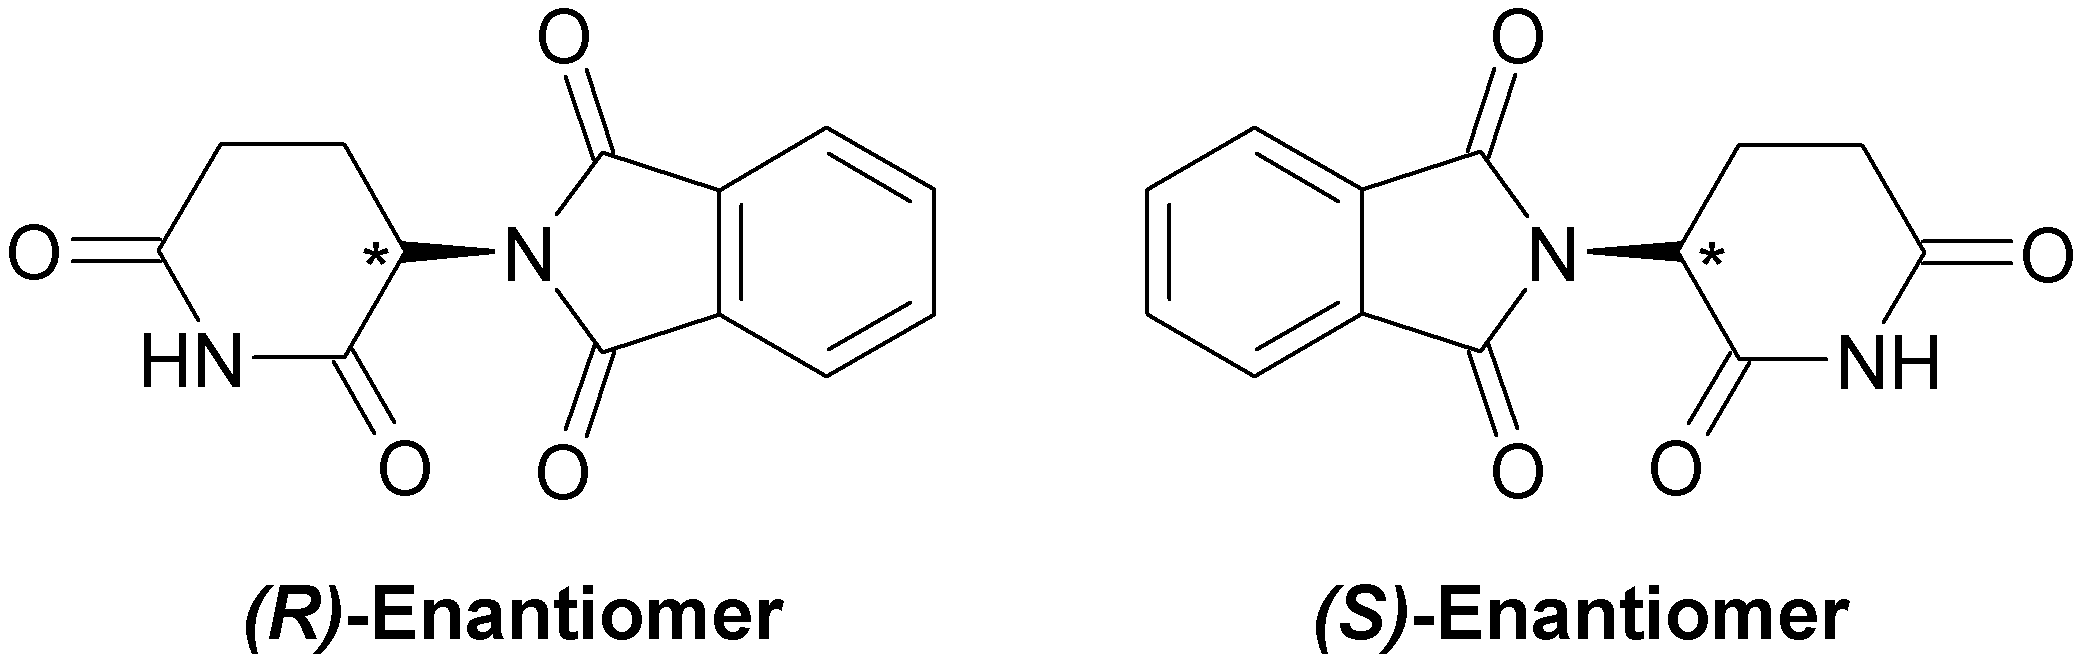
\includegraphics[width=0.5\linewidth]{thalidomide.png}
    \caption{The Tahlidomide molecule's two enantiomers.}
    \label{fig:thalidomide}
\end{figure}
Their relevance mainly comes in that the enzymes in biological organisms are very selective with the conformation of their substrate molecules, to the point that typically, only one of the enantiomers of the substrate molecule of the enzyme can link to its active region. This means that it can happen, and does happen, that one of the optical isomers affects in a way, while the other one affects the organism in a very different way. The consequences in medicine are dramatic. There is this lesson given by history to the pharmaceutical industry that every organic chemistry student is told about: the Thalidomide. It was released as a drug to alleviate nausea in pregnant woman. It turned out one of the optical isomers did indeed cure nausea, but the other one disrupted the limb growth of human embryos. It is since crucial for any pharmaceutical company to constantly monitor the enantiomer proportion of their medicines, for which the only way we have is to measure the LP of light. 


\item {\bf Example in Experimental Chemistry: }The same reasoning allows the measurement of the concentration of any particular chiral molecule in a solution, by measuring the rotation of LP light it induces \cite{concentration1, concentration2}. This method is non-invasive with the solution and can be fast enough for real time monitoring of the concentration of the chiral molecule. This is then useful for example to determine kinetic constants of chemical reactions \cite{enantiomers}.

\item {\bf Example in the Food and Beverage Industry:} The exact same reasoning also implies that living organisms have a preference for one of the enantiomers (for they should other-wise have two versions of many enzyme). This causes for example that only D-glucose is naturally synthesized and although it is indistinguishable in taste, L-glucose cannot be digested (and used as energy source). It is then typical in the food industry to monitor the concentration of sugar using linear polarization \cite{manual}.

\item {\bf Example in Astronomy: } Following Refs. \cite{exoplanets, exoplanets2}, LP measurements can be used to characterize exoplanets. The light reflected from a planet, lighted by its own star, is linearly polarized by its interaction with the atmosphere, as opposed to the unpolarized light originally emitted by the star. The degree of polarization is proportional to the reflecting surface, as one of the few indicators of the size of the atmosphere over the opaque core of the planet. Not only that, but the wavelength at which the phenomenon occurs most strongly, indicates the size and thus the possible composition of the particles in the atmosphere (apart from {\bf the color of its sky}). In addition, the maximum degree of polarization is achieved when the planet reflects light to Earth at a 90 degree angle. This happens when the planet is at the maximum visual separation from the star as seen from the Earth, happening twice every orbit. Therefore, the measurement of LP can even be used to characterize the period of the orbit of an exoplanet.
\end{itemize}

Among other equally interesting applications of the live measurement of LP, there are remote sensing applications \cite{remote} or the contrast enhancement of medicinal images \cite{contrast}. For all of these applications and more, a cheap, portable, precise and fast LP polarimeter would definitively be a revolution.


\newpage

\fancyhead[OR]{ }
\fancyhead[EL]{}
\fancyhead[OL]{ }
\fancyhead[ER]{}
\newpage
\null
\newpage
%%%%%%%%%%%%%%%%%%%%%%%%%%%%%%%%%%%%%%%%%%%%%%%%%%%%%%%%%%%%%%%%%%%%%%%%%%%%%%%%%%%%%%%%%%%%%%%%%%%%%%%%%%%%%%%%%%%%%%%%%%%%%%%%%%%%%%%%%%%%%%%%%%%%%%%%%%%%%%%%%%%%%%%%%%%%%
%\newpage


%\begin{kapituloBerria}{Part B}{ The Path Towards a Fully Functional Portable Prototype}
%Designing the Hardware
%\end{kapituloBerria}
%\newpage
%\fancyhead[L]{\null}
%\fancyhead[R]{\null}
%\null
%\clearpage



%%%%%%%%%%%%%%%%%%%%%%%%%%%%%%%%%%%%%%%%%%%%%%%%%%%%%%%%%%%%%%%%%%%%%%%%%%%%%%%%%%%%%%%%%%%%%%%%%%%%%%%%%%%%%%%%%%%%%%%%%%%%%%%%%%%%%%%%%%%%%%%%%%%%%%%%%%%%%%%%%%%%%%%%%%%%%
\newpage


%\begin{kapituloBerria}{Part C}{ From Crescent Ring Images to Polarization Angle Differences }
%Designing the Software
%\end{kapituloBerria}
%\newpage
\fancyhead[L]{\null}
\fancyhead[R]{\null}
%\null
%\clearpage


\section*{\centering \huge{Part B: The Mind of the Polarimeter}\vspace{-0.3cm}}
\addcontentsline{toc}{section}{Part B: The Mind of the Polarimeter}
\noindent\rule{\textwidth}{0.4pt}

In this section, we will focus our attention in the description of the developed computational solutions to determine the CR crescent ring orientation and the LP of the input light beam. Since for any reasonable measurement of LP, we need to measure it against the LP of a reference beam, we will assume in our discussion that we have two images: the crescent ring generated by the reference light beam and the one generated by the problem light beam. We will call them {\bf the reference} and {\bf the problem} images. Our objective is to get the relative LP angle between the incident reference and problem beams, which we will denote by $\Delta \Phi_{LP}$.

For notational convenience, let us define some important features of the CR crescent ring images:\vspace{-0.15cm}
\begin{itemize}
\item We will denote by $I$ the intensity of light of the captured transversal section with the camera. Since the images are captured with 8 bits in the experiments, we will assume that $I$ only takes one among 256 possible intensity values. Then, the image would be given by a function $I(x,y)$ with the coordinates $\vec{q}:=(x,y)\in\Omega\subset \mathbb{Z}$ denoting the pixel coordinates of the image, for a certain rectangle $\Omega=\{(x,y)\in\mathbb{Z}:0\leq x\leq W\;\&\;0\leq y\leq H\}$, where $H,W$ are the {\bf height and width} of the images (the number of capturing elements of the camera in each axis of the rectangular sensor). Note that the pixel coordinate system, as typically done for computational arrays is centered in the top left corner of the image. These coordinates $(x,y)$ represent the rows $y$ and columns $x$ of the image matrix.


\item We will denote by $\vec{g}_{geom}$ the {\bf geometrical center} of the crescent ring. It is defined as the point where the center of mass of the intensity image for an input CP would lay (for the full hollow ring). It is the intersection of the central axis of the cone and the constant $z$ plane. Since the experimental images can land, from an analyzed sample to the next one in different positions of the camera plane, it is something {\bf a priori we must assume to be unknown}.

\item We will denote by $\vec{g}_{grav}$ the gravitational center, center of mass or {\bf gravicenter} of the crescent ring image. It is given by:\vspace{-0.05cm}
\begin{equation}\label{grav}
\vec{g}_{grav}:=\frac{\sum_{(x,y)\in\Omega} I(x,y)\vec{q}}{\sum_{(x,y)\in\Omega}I(x,y)}\vspace{0.05cm}
\end{equation}
Unlike the geometrical center, the gravicenter is trivially computable in any experimental image.

\item For a generic crescent ring image, we will denote by $\Phi_{LP}$ {\bf the angle the input light's linear polarization plane makes with the $x$ axis} of the camera's sensor, such that $\Phi_{LP}\in(-\pi/2,\pi/2]$. We can see from equation \eqref{cosine} that the angle defined as $\phi_{CR}:=2\Phi_{LP}$ will then be {\bf the angular distance at which the peak of the CR crescent ring lands} relative to the $x$ axis of the camera sensor (assuming we center the polar coordinates in the geometric center of the ring). In particular, the relative LP angle between the problem and reference images will be given by $\Delta \phi_{CR}/2:=(\phi_{CR_{pb}}-\phi_{CR_{ref}})/2=\Phi_{LP_{pb}}-\Phi_{LP_{ref}}=:\Delta \Phi_{LP}$, where the sub-indices $pb,ref$ refer to the problem and reference rings respectively. Since typically we will compute $\phi_{CR_{pb}},\phi_{CR_{ref}}$ first, in order to have all relative angles $\Delta \Phi_{LP}$ in the same branch $(-\pi/2,\pi/2]$, we will make sure that any $\phi_{CR}$ angle is taken to $(-\pi,\pi]$. For this, Algorithm \ref{alg:topipi} is employed.\vspace{-0.02cm}
\SetKwComment{Comment}{\# }{ \#}
\SetKwProg{func}{Def}{ }{}
\SetKwProg{Given}{Given}{ }{}

\begin{algorithm}
{\small \caption{ \rule{0pt}{3mm}{}Take angle $\phi\in\R$ to $(-\pi,\pi]$}\label{alg:topipi}
\Given{ $\phi\ :$}{
$\phi\gets \phi\ mod\ (2\pi)$\Comment*[r]{Take it to (-2pi,2pi)}
\uIf{abs(\ $\phi$\ )$\ >\pi$}{{\bf return } $\phi-$sign$(\phi)\cdot 2\pi$\;}
\uElse{{\bf return }$\phi $ \Comment*[r]{Already in (-pi,pi)}}}}
\end{algorithm}

%\vspace{-0.2cm}

\end{itemize}
\SetKwComment{Comment}{\# }{ \#}
\SetKwComment{CommentMath}{\text{\# }}{\text{ \#}}
\SetKwProg{func}{Def}{ }{}
\SetKwProg{Given}{Given}{ }{}

\section*{B.1. The Computer Vision Task and the General Quandary}
\addcontentsline{toc}{subsection}{1. The Computer Vision Task and the General Quandary}
The computer vision problem seems simple: we have a pair of crescent-moon-like images for which we wish to know the relative angle at which they have their crest's maximum intensity points $\Delta \phi_{CR}$. Half this relative rotation will give us the relative linear polarization angle between the input light beams $\Delta \Phi_{LP}$. As derived in Part A, these CR crescent rings are expected to have very nice {\bf geometrical properties}. Among others:
\begin{itemize}
\item[\bf (a)] Each of them should be symmetric with respect to the axis crossing the geometric center and the maximum and minimum intensity spots along the ring. We will call this the {\bf main (symmetry) axis} of the crescent ring.
\item[\bf (b)] The gravicenter $\vec{g}_{grav}$ is aligned with the geometric center $\vec{g}_{geom}$ along the main axis.
\item[\bf (c)] Following equation \eqref{cosine}, the angular histogram obtained by radially integrating the images from the geometric center should have a squared cosine shape. Moreover, the cosine should be angularly displaced exactly double the polarization angle $\Phi_{LP}$.
\item[\bf (d)] If the problem and reference LP-s differ by $\pi/2$ radians, that is, they are orthogonal polarizations, adding their CR rings pixel-wise, after centering both in their geometric centers, we should get a constant angular intensity profile. To see this, recalling equation \eqref{cosine}:
\begin{equation}
\mathcal{I}_{\Phi_{LP}}(\varphi;z)+\mathcal{I}_{\Phi_{LP}+\pi/2}(\varphi;z) = C(z)cos^2(\varphi/2-\Phi_{LP})+C(z)(cos^2(\varphi/2-\Phi_{LP}-\pi/2)
\end{equation}
where using that $cos(x-\pi/2)=sin(x)$ and $sin^2(x)+cos^2(x)=1$, we get that: $\mathcal{I}_{\Phi_{LP}}(\varphi;z)+\mathcal{I}_{\Phi_{LP}+\pi}(\varphi;z) = C(z)$. This is a constant for a fixed $z$, as we wanted to prove. Its relevance is greater though. By recalling equation \eqref{yoyo}, we see $C(z)$ is the angular profile of the complete ring generated by an input CP.\footnote{By the linear decomposition of polarization in orthogonal components this was already trivial.} This implies an additional self-symmetry : the sum of a CR crescent ring with its $\pi$ rad rotated version, should give a complete uniform ring.
\fancyhead[OL]{\em Part B: The Mind of the Polarimeter}
\item[\bf (e)] It is worth noting another consequence of the previous points: if the experimental conditions are identical (meaning $R_0,w_0,z$ are fixed), the rings obtained by only changing $\Phi_{LP}$ should be exact rotated versions of each other.
\end{itemize}
\fancyhead[OR]{ The Computer Vision Task}
\fancyhead[EL]{ The Computer Vision Task}
\fancyhead[ER]{\em Bachelor's Thesis: Conical Refraction Polarimeter}

All these symmetries make the problem seem to be simple, and qualitatively it is. However, we are looking for the most {\bf quantitative} result possible. To put this into context, a mildly satisfactory result would be to be able to determine the relative angles to an error within $1$ degree, which are about $0.017$ rad. This would imply that we are looking to classify the crescent ring image pairs in at least 360 classes. Currently sold polarimeters however, as we have seen, correctly measure polarization variations in the second decimal place in degrees (the fourth place in radians). Thus, a really satisfactory classification would involve about 36000 classes. If the images were as symmetric as theoretically predicted, then the problem would still be rather simple. However, as we will review in section (C.2), the experimental crescent rings are very noisy. So noisy that actually not even a single theoretical symmetry mentioned above really holds. This renders the quantitativeness of a generic algorithm a significant number of orders of magnitude as we will see. Even still, we will develop all sorts of algorithms based on these symmetries.

As an additional handicap, in the limited time of the thesis, we lacked both experimental and computational resources. On the one hand, we did not have access to abundant certified ground truth LP beams, which are fundamental to know the real performance of the algorithms. They could even be useful to design models that learn to look through the experimental noise or even to mimic it. This lack of a big experimental labeled dataset, was the biggest of the problems. On the other hand, we had limited computational resources, for we only disposed of a single personal use GPU. This directly prunes many of the deep learning algorithms we could have employed.


With all this said, we still had a very relevant advantage in our favour: as we have explained in Part A, we know the phenomenon well enough as to be able to generate unlimited theoretically perfect simulated crescent ring images labeled with their associated parameters. We would then only need to also simulate the experimentally observed noise.
\vspace{-0.3cm}

\section*{B.2. Artificial Noise \vspace{-0.3cm}
}
\addcontentsline{toc}{subsection}{2. Artificial Noise}
\fancyhead[OR]{ Artificial Noise}
\fancyhead[EL]{ Artificial Noise}
Experimental noise had to be simulated for the theoretically perfect images in order to have labeled samples that can  give us a realistic impression of how well the algorithms really perform when the theoretical symmetries are broken. Then, following the description of the experimentally found non-idealities in section (C.2), we attempt to mimic the experimental noise with the following ideas. We will denote by $I_{sim}$ the perfect theoretical simulated image, while by $\tilde{I}_{sim}$ its noisy version. Then:
\begin{enumerate}
\item In order to emulate the random "bites" the crests present in experimental images (see Figures \ref{fig:expnoise}.b and c), we will randomly modulate the image with some Gaussian shape blobs. To do this:
\begin{enumerate}
\item We choose a random number $K$ between 0 and 3, representing the number of 2D Gaussian blobs, and we fix a random maximum relative blob strength $c$ in $(0,0.5)$. We also sample a "strength" number $\alpha_k$ in (0,1) for each blob, and we normalize them to form a unit vector (in order to have the total blob density be normalized).
\item We choose the center of each Gaussian, $(\mu_{xk},\mu_{yk})$, by sampling randomly $K$ points in the support of the image $(\vec{x},\vec{y})$, with probability function given by the intensity at each point $I_{sim}(\vec{x},	\vec{y})$. We do so, because we observed that the "bites" most likely appear in the regions where the intensity is expected to be higher. In addition, we sample the standard deviations, $(\sigma_{xk},\sigma_{yk})$, uniformly in the square $(100,130)\cross(100,130)$. These sizes were found to mimic well the "bites" of experimental samples for 541$\times$541 simulated images.
\item We compute the blob mask as:\vspace{-0.2cm}
\begin{equation}
B(x,y)=\sum_{k=1}^K \frac{\alpha_k}{2\pi\sigma_{xk}\sigma_{yk}}e^{-\frac{(x-\mu_{xk})^2}{2\sigma_{xk}^2}-\frac{(y-\mu_{yk})^2}{2\sigma_{yk}^2}}
\end{equation}
and then divide it by its maximum value, so it is ranged in $[0,1]$.
\item Finally we distort the image as: $
\tilde{I}_s(x,y)=I_s(x,y)\qty(1-cB(x,y))$.
\end{enumerate}
\item In order to account for the second most notable noise type, by which the ring crests show random oscillations (see Figure \ref{fig:expnoise}.a), we now distort the images with a pseudo-random oscillation:
\begin{enumerate}
\item Sample three random frequencies $f_k$ uniformly in ($\pi/3,\pi$). This range is chosen to make the generated noise be as similar to the experimental noise as possible. Sample as well three random frequency strengths $\alpha_k$ in (0,1) and normalize them as a vector to unit norm. In addition, fix a maximum noise factor $c$ sampling it from $(0,0.5)$.
\item Compute the polar angle of each pixel position $\varphi(x,y)$, relative to the geometrical center of the image $\vec{g}_{geom}$.
\item Then apply the next pseudo-random oscillatory modulation to the image:
\begin{equation}\hspace*{-0.6cm}
\tilde{I}_{sim}(x,y) = \tilde{I}_{sim}(x,y)\qty{1-c[\alpha_1cos(f_1\varphi(x,y)) +\alpha_2sin(f_2\varphi(x,y)) +\alpha_3cos(f_3\varphi(x,y))]^2}
\end{equation}
\end{enumerate}
\item Following when each noise is introduced in the experiments, we account for Poissian noise as the last noise factor. For this, we consider $I_s(x,y)$ to be the expected number of counts to be received in the $x,y$ pixel. Then, we shot-noise the already spoiled image by first sampling a random strength of the Poisson noise $c$ in $(0,0.5)$ and then applying: $\tilde{I}_{sim}=(1-c)\tilde{I}_{sim}+cP(I(x,y))$. $P(\lambda)$ represents a random sample from a Poisson distribution of parameter $\lambda$.
\end{enumerate}
Example representative simulated noisy images can be found in Figure \ref{fig:artifNoise}. Note that indeed, they are similar to the experimental noises of Figure \ref{fig:expnoise}.

\begin{figure}[h!] 
     \centering 
    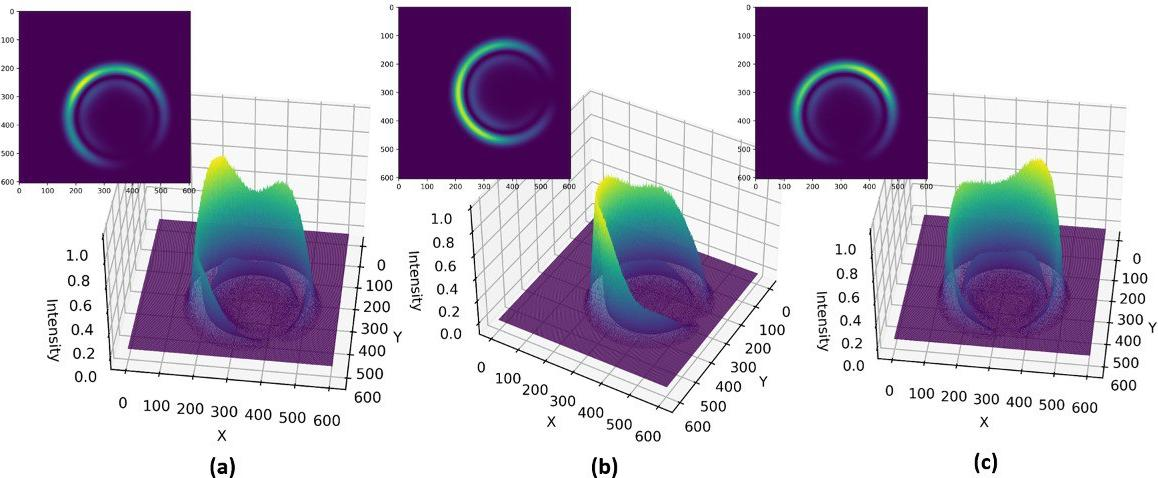
\includegraphics[width=0.92\linewidth]{artif.jpg}
    \caption{Representative examples of random simulated noisy images, plotted as heatmap and surface plots.}
    \label{fig:artifNoise}
\end{figure}

\section*{B.3. The Simulated Image Datasets }
\addcontentsline{toc}{subsection}{3. The Simulated Image Datasets}
\fancyhead[OR]{ The Simulated Image Datasets}
\fancyhead[EL]{ The Simulated Image Datasets}
The small labeled experimental image datasets of section (C.3) should only be used as a decisive benchmark. Thus, we generate several simulated image datasets, each of them with (for our purposes) an unlimited (about 1e6) number of labeled samples. For the storage of the resulting image- and label-arrays the {\em HDF5} binary data format was employed, managed in Python by the {\em h5py} library \cite{h5f}.\vspace{-0.1cm}
\begin{itemize}
\item {\bf Mother Dataset :} The numerical computation of each simulated image takes a considerable amount of time. The bottleneck is the computation of the $B_0,B_1$ integrals\footnote{We did not have the chance to properly GPU parallelize the computation of the Bessel functions.}. Once we have $B_0,B_1$, CR rings for arbitrary Jones vectors can instantly be generated. In particular, it is convenient to pre-compute the matrix that in equation \eqref{master} appears getting multiplied with the Jones vector, which we will call {\bf the $D$ matrix}\footnote{For it is the last preamble to obtain the displacement $\vec{D}$.}, for several $R_0,w_0,z$ in a given grid. This is the content of the Mother Dataset. The grid of possible $R_0,w_0,z$ was designed around the experimentally found average parameters (a slightly wider range to test the robustness of the algorithms). It contains 115 equispaced $R_0$ in $(110,180)$, 115 $w_0$ in $(8,35)$ and 3 $z$ in $(0,0.05)$ $-$ so few $z$ values are considered because setting the camera in the focal plane is a task we can perform with great accuracy. Each $D$ matrix is linked to its ground truth $R_0,w_0,z,\phi_{CR}$ in the dataset, which can thus be used as a look-up table in the Simulation Fit algorithms (B.9).

\item {\bf Non Noisy Image Dataset:} Using the Mother Dataset, a huge library of random simulated images was generated, both in 8 bit {\em .png} format and the $HDF5$ format. All images were generated without noise and with the ground truth $\phi_{CR}$ labeling them. The images are normalized to their maximum possible value (255 for 8 bits). The objective of this dataset is to test how the algorithms perform in the most ideal of the conditions, but for random ring parameters. Note that the library contains $R_0,w_0,z,\phi_{CR}$ of any value in the Mother Dataset's grid, even if in the actual device, this range is quite controlled. 

\item {\bf Noisy Image Dataset:} Using the Mother Dataset, a dataset with the same features as the previous Non Noisy Image Dataset was generated, but now applying the random artificial noise to each image. The parameters of the noise were set to produce significantly noisier images than the experimental ones, since the objective of this dataset is to test the robustness of the algorithms in front of the worst-case-scenarios.

\item {\bf Variant Image Dataset:} A special dataset was generated to train the triplet loss embedder that we will explain in (B.8). It contains multiple different noisy versions of the same non-noisy images batched together and labeled by their common $\phi_{CR}$ ground-truth.
\end{itemize}
\newpage
\section*{B.4. Preprocessing }\vspace{-0.1cm}
\addcontentsline{toc}{subsection}{4. Preprocessing}
\fancyhead[OR]{ Preprocessing}
\fancyhead[EL]{ Preprocessing}
Because the rings can appear centered quite randomly in the experimental images, in order for them to be comparable it is convenient to standardize them somehow. For this we suggest the method we named $iX$ or Kalkandjiev standard (for it was thought by Prof. Todor K. Kalkandjiev).\vspace{-0.35cm}
\subsubsection*{The Kalkandjiev-iX Standard\vspace{-0.15cm}}
The gravicenter of the image is trivial to be computed using equation \eqref{grav}. Then the $iX$ standard converts the image to a square $(2X+1)\cross(2X+1)$ image with the gravicenter in the center of it, with $X\in\N$ pixels to the left, right, above and below. The first thing is to choose an $X$ value such that the rings of the range captured by the camera can fit in. The procedure is to create a $2X+1$ side square blank array, where by an output-to-input strategy we set the gravicenter rounded to the nearest whole integer in the $(X+1,X+1)$-th pixel. The details can be found in Algorithm \ref{alg:iX}\footnote{Note that in every Algorithm box, we will assume the arrays start indexing at 0 and the -1 index is the last element. Then, the range of indices $i:j$ goes from $i$ until $j$, including $j-1$ but not $j$.}. In our case, since the employed camera has a resolution of $720\cross 540$, we decided to use $X=302$, such that the resulting image of size $605\cross 605$ could embody any reasonable gravicenter-centered ring. Note that the rings of the iX images are tilted towards the maximum intensity direction, which is why a bit more than 540 pixels in each side were necessary.

\begin{algorithm}
\caption{\rule{0pt}{3mm}{} Convert Image to {\bf Kalkandjiev-iX Standard} - High Level Pseudocode }\label{alg:iX}
{	\small %\normalsize
\Given{$I,\ X$}{
$\vec{g}\gets$ compute gravicenter $(I)$\;
$iX\gets$ empty array of size $[2X+1,\ 2X+1]$\;
$\vec{l},\ \vec{u}\ \gets\ \vec{g}-X,\ \vec{g}+X+1$\;
$\vec{lb},\ \vec{ub}\gets\ $ clip to range [0, $shape(I)$] ($\vec{l},\ \vec{u}$)\;
$pad_{low},\ \gets \vec{lb}-\vec{l} $\;
$pad_{up},\ \gets \vec{ub}-\vec{u} $\;
$iX[\ pad_{low}[0]:pad_{up}[0],\ pad_{low}[1]:pad_{up}[1]\ ]\gets\ I[\ \vec{lb}[0]:\vec{ub}[0],\ \vec{lb}[1]:\vec{ub}[1] \ ]$\;
{\bf return }$iX$\vspace{0.1cm}
} }
\end{algorithm}


Now, assuming the images are set in the common $iX$ geometry, we can try to alleviate part of the noise and try to recover some of the symmetries of the images using pre-processing techniques before feeding the $\Delta \Phi_{LP}$ extraction algorithms. Let us describe the pre-processing techniques we implemented. We will denote by $I_p(x,y)$ the post-processed version of $I(x,y)$.\vspace{-0.35cm}

\subsubsection*{Normalize to Maximum Intensity}\vspace{-0.3cm}
Because experimental images may be taken with different exposure times and the input laser beam's intensity might fluctuate significantly from image to image, it is important to have a way to scale the rings "vertically" (in the intensity axis) in a common manner. For some of the algorithms, like the Simulation Fit or the Relative Rotation this will be a necessity. The procedure is simple: $I_p(x,y) = I(x,y)/max[I(x,y)]$. It takes the image to the range $[0,1]$. Its application on the experimental images of Figure \ref{fig:expnoise} can be seen in Figure \ref{fig:preprocessingMax}.\vspace{-0.3cm}


\begin{figure}[h!] 
     \centering 
    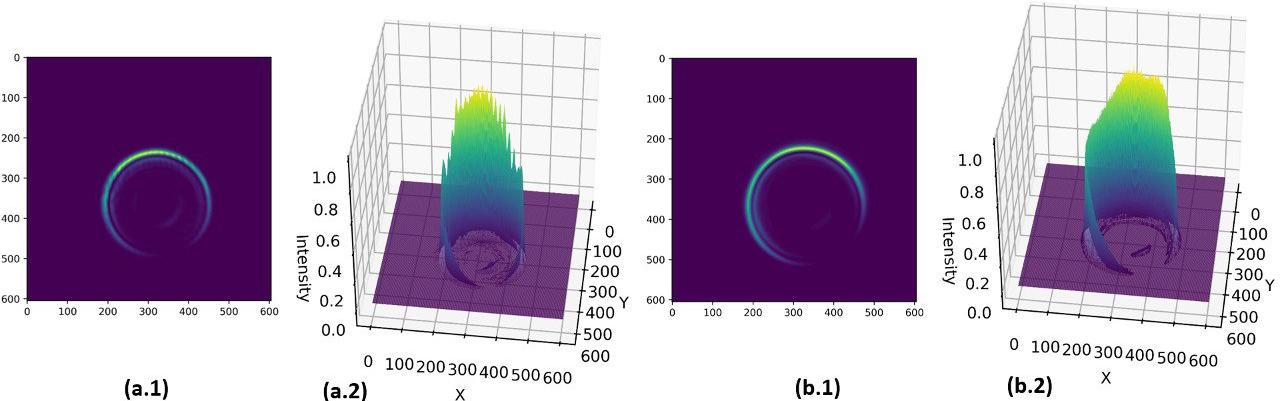
\includegraphics[width=0.9\linewidth]{max.jpg}
    \caption{"Normalize to Maximum Intensity" pre-processing applied on the the experimental images of Figure \ref{fig:expnoise}.}\vspace{-0.2cm}
    \label{fig:preprocessingMax}
\end{figure}

\subsubsection*{Normalize to Maximum and then to Mean}\vspace{-0.3cm}
The normalization to maximum is very prone to biased results when it is the maximum of the ring that has been damaged by noise (which turns out to be the case most of the times). As an alternative, we could normalize the image to its mean intensity value after being normalized to its maximum value. $I_p(x,y) = (I(x,y)/max[I(x,y)])/mean\{I(x,y)/max[I(x,y)]\}$. This should be robuster because the average intensity is harder to be corrupted than the single maximum point of the image. 

\subsubsection*{Saturate at a Threshold Intensity}\vspace{-0.3cm}
Because the information in the crests is typically very corrupted, a pre-processing that gave good results for some algorithms was to almost binarize the image. To leave only the bottom part of the image in terms of intensity. That is, to clip all the intensity values that were bigger than a certain ratio $t\in(0,1)$ of the maximum intensity value, and then to normalize the whole to unity: $I_p(x,y)=least[I(x,y)/max[I(x,y)],\ t]/t$. It is not exactly a binarization of the image because the curves at the bottom in $I$ (below the threshold) are still preserved, as can be seen in Figure \ref{fig:preprocessingThresh}. Only very low thresholds (like $t=0.05$) gave good enough results.
\begin{figure}[h!] 
     \centering 
    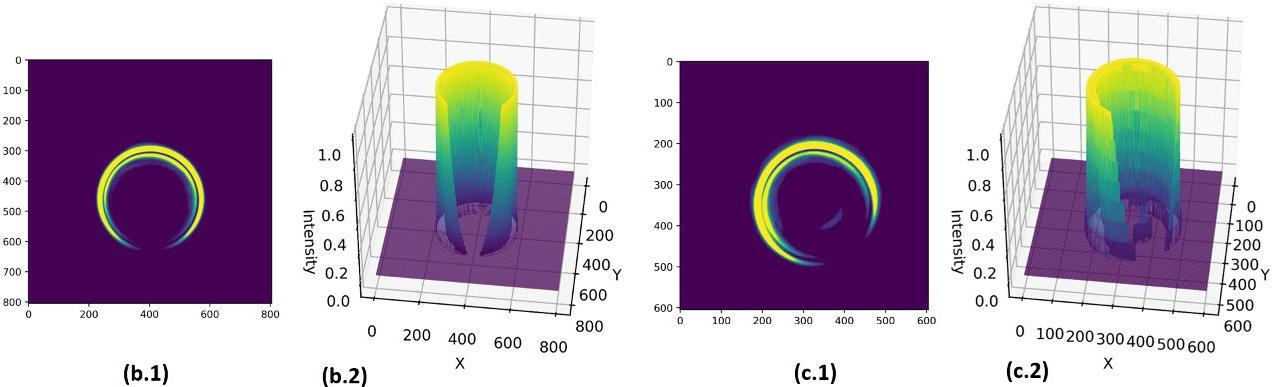
\includegraphics[width=0.9\linewidth]{thresh.jpg}
    \caption{"Saturate at Threshold Intensity" pre-processing applied on the experimental images of Figure \ref{fig:expnoise}.}
    \label{fig:preprocessingThresh} \vspace{-0.65cm}
\end{figure}


\subsubsection*{Sigmoid Transformation}
\vspace{-0.3cm}
A smoother and differentiable version of the threshold clipping is to apply a functional transformation to each intensity value, by which the lower parts of the crest are given more weight. The sigmoid is one such transformation: $I_p(x,y)=\frac{1}{1+exp(-k(I(x,y)/max[I(x,y)]-c))}$. It leaves two free parameters however: the central point of the sigmoid $c$ (analogous to the thershold) and its "slope" $k$. It will tend towards a strict binarization as $k\rightarrow \infty$. See examples in Figure \ref{fig:preprocessingSigmoid}.\vspace{-0.2cm}
\begin{figure}[h!] 
     \centering 
    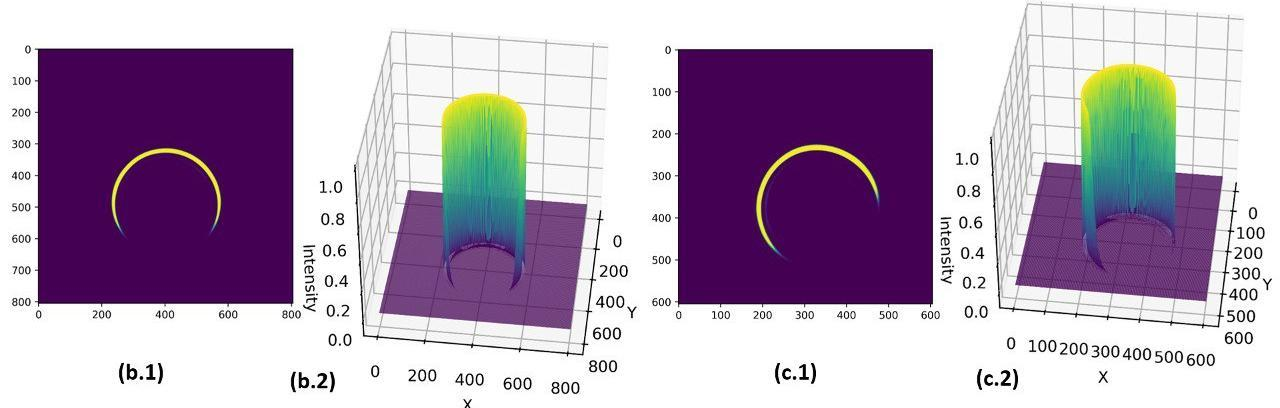
\includegraphics[width=0.9\linewidth]{sigmoid.jpg}
    \caption{"Sigmoid Transformation" pre-processing applied on the experimental images of Figure \ref{fig:expnoise}.}
    \label{fig:preprocessingSigmoid}
\end{figure}

\subsubsection*{Morphological Opening}\vspace{-0.25cm}
Both the threshold saturation and the sigmoid act as almost-binarizations segmentating the crescent moons. These segmentations are however performed in a global manner: without taking into account that there could be regions of the image with locally varying ranges of intensity. There could, for example, be a hole in the case of the device introducing an asymmetric background light. Then, a robuster method (that is also more computationally costly) to erase the crests of the rings, is to apply a morphological grayscale opening to the image \cite{opening}. This operation moves a sliding structuring element around the image that first erodes morphologically the image and then dilates it, getting rid of the so called "top-hats" or local maximums (which in our case are the irregular crests). $I_p(x,y)=Dilate[Erode[I(x,y)]]$. The size of the structuring element will determine the width of the local maximums or "hats" that will be erased. We find values between 7 and 11 pixels to be fine. See some examples in Figure \ref{fig:preprocessingOpening}.

\begin{figure}[h!] 
     \centering 
    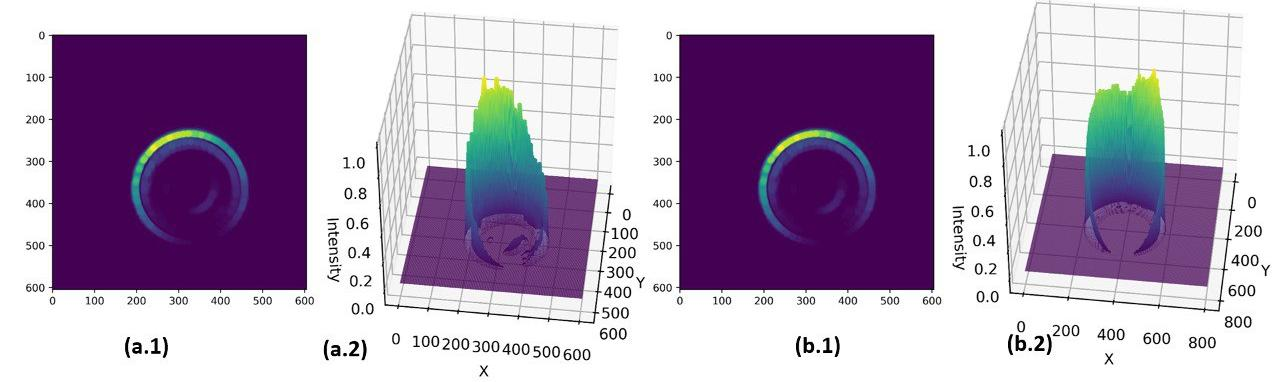
\includegraphics[width=0.9\linewidth]{open.jpg}
    \caption{"Morphological Opening" pre-processing applied on the experimental images of Figure \ref{fig:expnoise}.}
    \label{fig:preprocessingOpening}
\end{figure}\vspace{-0.5cm}

\section*{B.5. Optimization Algorithms\vspace{-0.2cm}}
\addcontentsline{toc}{subsection}{5. Optimization Algorithms}
 Before jumping to the implemented algorithms that obtain $\Delta\Phi_{LP}$, let us describe the implemented optimizers. Most of the algorithms we designed require an optimization step to find the $\phi_{CR}$ angle by  the minimization of a certain cost function $C(\vec{x})$ specific to the algorithm. Several of them only involve a one dimensional search space $x\in\Gamma\subset\R$, while some others involve a multidimensional search $\vec{x}\in\Delta\subset \R^n$ with $n>1$. Because for 1D minimization there are simple efficient algorithms, we implemented them separately, and only used the multidimensional ones when really required. In any of the cases, the cost function was a black-box function for which we do not know the analytic formula, nor we have the chance to have an explicit gradient.\vspace{-0.25cm}
\fancyhead[OR]{ Optimization Algorithms}
\fancyhead[EL]{ Optimization Algorithms}

\subsection*{B.5.1. One Dimensional Optimization Algorithms\vspace{-0.2cm}}
These optimizers were implemented in a common Python interface to be used with any of the algorithms in a same standing. We will denote by $x$ the support of the general continuous cost function $C(x)$, which is assumed to have at least a local minimum. It is important to note that any of the following algorithms will only find one local minimum, which need not be the one we are looking for.\vspace{-0.5cm}
\subsubsection*{Quadratic Fit Search}\vspace{-0.25cm}
If we have three points $x_1^{(0)}<x_2^{(0)}<x_3^{(0)}$ such that $C(x_1^{(0)})>C(x_3^{(0)})<C(x_2^{(0)})$, we know that by continuity of $C$ there is a minimum in the interval $(x_1^{(0)},x_3^{(0)})$. There is a unique parabola $P(x)=ax^2+bx+c$ with $a,b,c\in\R$ interpolating these points. Because they do not lay in a straight line, $a\neq 0$, we have an immediate formula for the minimum of this parabola $P'(x)=2ax+b\Rightarrow P'(x_4^{(0)})=0\Leftrightarrow x_4^{(0)}=-b/(2a)$. Then, $x_4^{(0)}$ necessarily lays in the interval $(x_1^{(0)}, x_3^{(0)})$ due to the conditon on $C$ for the three interpolated nodes. If we evaluate $C(x_4^{(0)})$ we now have the evaluations of 4 ordered points in $[x_1^{(0)},x_3^{(0)}]$. We choose the first three or the last three of them, which we will call $x_1^{(1)}<x_2^{(1)}< x_3^{(1)}$, requiring them to fulfill $C(x_1^{(1)})>C(x_2^{(1)})< C(x_3^{(1)})$. We have now bounded the minimum in a shorter interval. Then we start back, and iterate until the desired convergence criterion is hit. In each iteration, the interval in which we know there is a minimum is strictly contracted, so the convergence is guaranteed unless at some point $x_4^{(k)}=x_2^{(k)}$, in which case the procedure stops. This however is a very unlikely case given we work with real numbers. This is a well known algorithm that can be found in introductory optimization books like \cite{opt}. 

By imposing the interpolation conditions, we get an equation system with 3 unknowns $a,b,c$, which can be analytically solved, and used to evaluate directly $x_4^{(k+1)}$ as:\vspace{-0.2cm}
\begin{equation}\label{par}
x_4^{(k+1)}=(x_1^{(k)}-x_3^{(k)})(x_2^{(k)}-x_3^{(k)})\qty(\frac{x_1^{(k)}(C_3^{(k)}-C_2^{(k)})+x_2^{(k)}(C_1^{(k)}-C_3^{(k)})}{C_2^{(k)}-C_1^{(k)}}+C_3^{(k)})^{-1}\vspace{-0.2cm}
\end{equation}
where we denoted $C_j^{(k)}:=C(x_j^{(k)})$. Our implementation is found in Algorithm \ref{alg:qfs}. Note that the initial interval in which we bound the minimum $(x_{min},x_{max})$ will be dependent on the cost function and its semantic meaning.

\begin{algorithm}[h!]
\caption{\rule{0pt}{3mm}{} {\bf Quadratic Fit Search} - Our Implementation's High Level Pseudo-code}\label{alg:qfs}
{\small 
\Given{  $C(\cdot)$, $\Delta x$, $max\_its$, $C\_tol$,  $initial\_guess$, $x_{min}$, $x_{max}$}{
$x_{j}s,\ C_{j}s \gets initialize\_points(initial\_guess, x_{min},x_{max}, C)$\; \DontPrintSemicolon{\Comment*[r]{\footnotesize $x_js,\ C_js$ are valid initial point- and respective cost-arrays with 4 points}}
$it\gets 1$\;
\While{$it\leq max\_its$ and $abs(C_{j}s[k+1]-C_{j}s[k])>(C\_tol\:abs(C_{j}s[k]))$ and $abs(x_{j}s[k+1]-x_{j}s[k])>\Delta x\quad \forall k\in\{0,1,2\}$:}{
$j_{min}\gets argmin(C_js)+1$\;
$x_js[:3]\gets x_js[(j_{min}-1):(j_{min}+1)]$\;
$C_js[:3]\gets C_js[(j_{min}-1):(j_{min}+1)]$\;
$x_js[3] \gets$ min of interpolating parabola $(x_js[:3],\ C_js[:3])$\Comment*[r]{\small Using equation \eqref{par}}
$C_js[3]=C(x_js[3])$\;
$x_js,\ C_js\gets$ order arrays as would order $xjs$ $(x_js,C_js)$\;
$it\gets it+1$\;
}
{\bf return } $x_js[argmin(C_js)]$\vspace{0.1cm}
}}
\end{algorithm}
\vspace{-0.25cm}


\subsubsection*{Fibonacci Ratio Search}\vspace{-0.25cm}

Following the rationale of the quadratic fit search, given three points $x_1^{(0)}<x_2^{(0)}<x_3^{(0)}$ such that $C(x_1^{(0)})>C(x_3^{(0)})<C(x_2^{(0)})$, we know that by continuity there is a minimum in the interval $(x_1^{(0)},x_3^{(0)})$. Moreover, if we evaluate the cost at a random point in that interval, we will get four points such that unless the new point has the same cost as $x_2^{(0)}$, it will allow us to reduce the interval in which we know there is a minimum {\bf for sure}. We will just need to choose the first three or the last three points such that $x_1^{(1)}<x_2^{(1)}< x_3^{(1)}$, as a function of which ones fulfill that $C(x_1^{(1)})>C(x_2^{(1)})< C(x_3^{(1)})$. Now, the question is: could we choose the evaluation point to ensure that the interval reduction will have maximum expectation? Indeed. If we just wanted to evaluate two points in addition to the two boundary ones $x_1,x_3$, we could maximize the interval reduction expectation by choosing both $x_2,x_4$ to be a tiny $\epsilon$ apart from the center of the interval, causing if the first three are the points in which we bound the minimum, a reduction of the interval of a ratio $1/2$ and if the last three are the good ones, a reduction $1/2$ as well. For any other pair of evaluations instead of these ones, we could obtain a case with a bigger reduction than $1/2$, but the other case will have a smaller reduction, since they must add up to 1. Then, the expected reduction will never be greater than 1/2. Now, imagine we have the three good points into which we contract the search interval. Two of them will be very close to each other (an $\epsilon$) apart. Thus, if we want to evaluate an additional point, then the expected reduction of the interval this time will be very poor.

We can solve the optimal sequence of evaluations as follows. The new point we evaluate in each iteration will need to be symmetric with respect to the middle of the interval in order to avoid an asymmetric reduction of the interval, which will never give a better expected reduction. Then, there is only one degree of freedom to optimize. Given the boundaries $x_1, x_3$, if we know the relative distance $\rho_1\in(0,0.5)$ from the interval boundaries at which we place the first two points $x_2,x_4$, we can immediately know which is the relative distance at which to evaluate the next points $\rho_2,\rho_3,...\in(0,1)$. This is becasue, as proven in the diagram of Figure \ref{fig:fibo}, they must follow $1-2\rho_k=(1-\rho_k)\rho_{k+1}\Rightarrow \rho_{k+1}=1-\rho_k/(1-\rho_k)$. Now, given we are ready to evaluate $N$ points, which is the optimal solution\begin{wrapfigure}{r}{0.51\textwidth}
     \centering 
    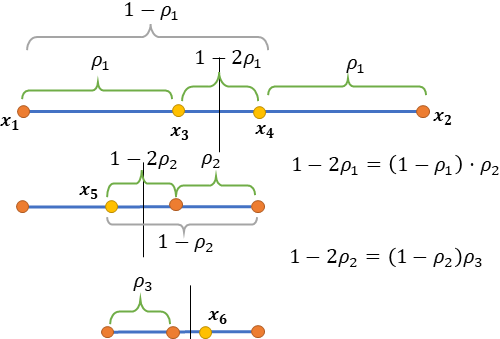
\includegraphics[width=\linewidth]{fibo.PNG}
    \caption{ Drawing of the iterative interval reduction proving the relation between reductions is $1-2\rho_k=(1-\rho_k)\rho_{k+1}$.}
    \label{fig:fibo}
\end{wrapfigure} $\rho_1$? The solution will be the minimum of the function $(1-\rho_1)\cdots(1-\rho_N)$, which is the total interval reduction factor achieved with $N$ evaluations. This is so irrespective of the decision we take in each iteration (about taking the first or the last three, for we made it symmetric). The minimization is subject to the restrictions $\rho_{k+1}=1-\rho_k/(1-\rho_k)$ and $\rho_k\in(0,0.5)$. The problem can be analytically solved using Karush–Kuhn–Tucker conditions, with a global minimum given by $\rho_k=1-F_{N-k+1}/F_{N-k+2}$ with $F_0=1,F_1=1$ and $F_{k+1}=F_k+F_{k-1}$ the Fibonacci succession. This is the well known Fibonacci search algorithm \cite{fibo, opt}. As expected, the last evaluation $\rho_N=1/2$ divides the interval by two. \newline $\null$\vspace{-0.35cm}



\begin{algorithm}[h!]
\caption{\rule{0pt}{3mm}{} {\bf Fibonacci Ratio Search} - Our Implementation's High Level Pseudo-code}\label{alg:fibo}
{\small
\Given{  $C(\cdot)$, $\Delta x$, $max\_its$, $C\_tol$,  $initial\_guess$, $x_{min}$, $x_{max}$ }{
$x_{j}s,\ C_{j}s \gets initialize\_points(initial\_guess, x_{min},x_{max}, C)$\; \DontPrintSemicolon{\Comment*[r]{\footnotesize $x_js,\ C_js$ are valid initial point- and respective cost-arrays with 4 points}}
$Fn\gets$ compute Fib. suc. until precis. $(\Delta x)$\Comment*[r]{\footnotesize Ordered Fib.suc.$\;$array with $	\frac{1}{Fn[-1]}<\Delta x$}
$it\gets 1$\;
\For{$it$ in $\{0,1,..., length(Fn)-1\}$}{
$\rho\gets 1-Fn[-1-it-1]/Fn[-1-it]$\;
$j_{min}\gets argmin(C_js)$\;
\uIf{$j_{min}==1$ }{ 
	\DontPrintSemicolon{\Comment*[r]{First 3 points}}
	\uIf{$\rho<1/3$}{
		$x_js[-1]\gets x_js[2]-\rho(x_js[2]-x_js[0])$\;		}
	\uElse{
		$x_js[-1]\gets x_js[0]-\rho(x_js[2]-x_js[0])$\;
		}
		$C_js[-1]\gets C(x_js[-1])$\;
}
\uElse{
	\DontPrintSemicolon{\Comment*[r]{Last 3 points}}
\uIf{$\rho>1/3$}{
		$x_js[0]\gets x_js[3]-\rho(x_js[3]-x_js[1])$\;		}
	\uElse{
		$x_js[0]\gets x_js[1]-\rho(x_js[3]-x_js[1])$\;
		}
		$C_js[0]\gets C(x_js[0])$\;
}

$x_js,\ C_js\gets$ order arrays as would order $xjs$ $(x_js,C_js)$\;
\uIf{$it\geq max\_its$ or $abs(C_{j}s[k+1]-C_{j}s[k])<(C\_tol\:abs(C_{j}s[k]))$ or $\null\hspace{0.8cm}abs(x_{j}s[k+1]-x_{j}s[k])<\Delta x\quad \forall k\in\{0,1,2\}$}{{\bf break}\;}
}
{\bf return } $x_js[argmin(C_js)]$\vspace{0.1cm}} }
\end{algorithm}\vspace{-0.2cm}

\noindent This allows us to know that the optimal strategy will reduce the interval by {\small $(1-\rho_1)\cdots(1-\rho_N)=1/F_{N+1}$}. Then, we can fix the uncertainty $\Delta x$ with which we wish to know the location of the local minimum, and get the number of evaluations $N$ required for it (computing the Fibonacci succession until $1/F_{N+1}$ is smaller than the desired precision). See our implementation in {\small Algorithm \ref{alg:fibo}.}\vspace{-0.3cm}
\subsection*{B.5.2. Multidimensional Optimization\vspace{-0.2cm}}
The multidimensional optimizers known as the Nelder-Mead method and the Powell method were found to be properly implemented in the {\em scikit-optimize} library for Python \cite{skopt}, so we did not implemented them. Let us thus, only explain them qualitatively.
\mybox{{\bf The Nelder-Mead or Tracker Simplex Method \cite{NM,opt}\vspace{0.2cm}}\\
Given the cost function $C(\vec{x}):\R^N\rightarrow\R$ to be minimized and a set of $N+1$ points $\{\vec{x}_j\}_{j=1}^N$ that form the vertices of an $N$-simplex (the polytope with least number of vertices and a non-zero $N$-volume that can be built), we make sure $\vec{x}_j$ are ordered by their cost functions as $C(\vec{x}_1\leq\cdots\leq C(\vec{x}_{N+1})$. Then, we compute the barycenter $\vec{x}_0$ of the hyperplane shaped by all the points $\vec{x}_j$ except the farthest in cost from the minimum: $\vec{x}_{N+1}$. We compute the "reflection" of $\vec{x}_{N+1}$ relative to the barycenter $\vec{x}_0$ as $\vec{x}_{refl}=\vec{x}_0+\alpha(\vec{x}_0-\vec{x}_{N+1})$ for a fixed $\alpha>0$. Then, we evaluate the cost at this reflected point. If it is lower than $\vec{x}_N$'s, replace $\vec{x}_{N+1}$ by $\vec{x}_0$ and go back to the beginning. If it is lower than the best so far, $\vec{x}_1$, then try to take a further step in that direction. If it is not better than $\vec{x}_N$, then take instead the point between the barycenter and $\vec{x}_{N+1}$ (using $\alpha\in(0,0.5)$); if better than $\vec{x}_{N+1}$, substitute it, else, shrink the whole simplex towards the best point $\vec{x}_1$. The algorithm can be made to converge when the simplex's volume is small enough, the cost values satisfy certain criteria etc. Graphically the method seems to evolve an $N$ dimensional "being" looking for the lowest temperature region, given by $C$.\vspace*{0.3cm}

{\bf Powell's Conjugate Direction Method \cite{P,opt} \vspace{0.2cm}\\}
For this method we begin with a point $\vec{x}_0$ and a set of $N$ linearly independent direction vectors $\{\vec{d}_j\}_{j=1}^N$. We perform a line optimization with a 1D otimizer (like the Fibonacci ratio search), over the line directed by the first vector $\vec{d}_1$ from $\vec{x}_0$. We take the minimum $\vec{x}_1$ and now perform a line optimization on the line that $\vec{x}_1$ forms in the direction $\vec{d}_2$. Continuing this process, we arrive at $\vec{x}_N$. Then we define a new direction $\vec{d}_{N+1}$ (a conjugate direction), as the one joining $\vec{x}_0$ and $\vec{x}_N$. We optimize the 1D slice in that direction and get $\vec{x}_{N+1}$. We now substitute the closest vector $\vec{d}_j$ to $\vec{d}_{N+1}$ by $\vec{d}_{N+1}$ and start again. Eventually some convergence criteria will be met.
}\vspace{-0.4cm}

\section*{B.6. Geometric Algorithms}
\addcontentsline{toc}{subsection}{6. Geometric Algorithms}
\fancyhead[OR]{ Geometric Algorithms}
\fancyhead[EL]{ Geometric Algorithms}
We designed the algorithms of this section to explicitly exploit the geometrical properties described in (B.1) in order to let us know $\Delta\Phi_{LP}$ from the crescent ring images. In what follows we will describe the inner workings of each one.\vspace{-0.35cm}

\subsection*{B.6.1. The Relative Rotation Algorithm \vspace{-0.2cm}}
One of the simplest ideas would be to use the fact that crescent rings for fixed experimental conditions, fixed $R_0,w_0,z$, should be exactly the same, only differing in a $\Delta\phi_{CR}$ rotation by their geometric centers (property (e)). The key point is that if we rotate the image instead about the gravicenter, we still get a match at an angle $\Delta\phi_{CR}$. Then, we could displace one of the rings to align its gravicenter with the other one's and rotate it about the new gravicenter, looking for the rotation angle that minimizes the difference between the two images. See Algorithm \ref{alg:relrot} for details. The 1D minimization of the similarity between the rotated problem and unrotated reference is done using one of the algorithms of (B.4.1). For this, we must define a similarity metric to be used as cost function. In general, unless stated otherwise, we will employ for all the algorithms the mean absolute error:

\begin{equation}\label{MAE} MAE\; [\ I_1(x,y),\ I_2(x,y)\ ]=\qty{\sum_{x,y}abs\qty(I_1(x,y)-I_2(x,y))}/\sum_{x,y}1\vspace{-0.25cm}
\end{equation}
\begin{algorithm}
\caption{ \rule{0pt}{3mm}{} {\bf The Relative Rotation Algorithm} - High Level Pseudo-Code}\label{alg:relrot}
\func{ $C(phi;\ I_{pb},\ I_{ref},\ \vec{g}_{pb},\ \vec{g}_{ref},\  similarity(\cdot,\cdot))$}{
	$pb\_rot \gets$ affine translat. and rot.$(I_{pb},\ $transl$=\vec{g}_{ref}-\vec{g}_{pb},\ $angl$=phi,\ $rot\_center$=\vec{g}_{ref})$\;
	{\bf return} -similarity($pb\_rot,I_{ref}$)\\
}
\vspace{0.2cm}
\Given{ $I_{pb},\ C,\ I_{ref},\ \vec{g}_{pb},\ \vec{g}_{ref},\  similarity(\cdot,\cdot),\ \phi_{min}:=-\pi,\ \phi_{max}:=\pi$\\ \DontPrintSemicolon{\CommentMath*[r]{$\vec{g}_{pb}, \vec{g}_{ref}$ are the gravicenters\vspace{-0.5cm}}}}{\vspace{0.1cm}
$I_{pb},I_{ref}\gets$ iX standard  $(I_{pb}),$ iX standard $(I_{ref})$\;
$w\gets\{\ I_{ref},\ \vec{g}_{pb},\ \vec{g}_{ref},\  similarity(\cdot,\cdot)\}$\;
$\Delta\phi_{CR}\gets$ 1D minimum Search $(C(\cdot;w), \phi_{min},\phi_{max})$\;
$\Delta \phi_{CR}\gets$ take to $(-\pi,\pi)$ with alg. \ref{alg:topipi}$\ \{\Delta \phi_{CR}\}$\;
{\bf return }$\Delta\phi_{CR}/2$\DontPrintSemicolon{\Comment*[r]{It returns $\Delta \Phi_{LP}$}}\vspace{0.1cm}
}
\end{algorithm}\vspace{-0.3cm}

The main complication affecting this algorithm is the fact that the noise in the experimental images does not rotate with the input beam's LP (since it is especially due to the stationary elements). Thus, the equality assumption is never really fulfilled.\vspace{0.35cm}

\mybox{{\bf Affine Transformations \vspace{0.2cm} \\}
Many of the algorithms employ image translations, rotations and mirror-flips. These can efficiently be performed employing matrix operations by considering the images to be in an affine space. Essentially, we will consider the plane of the images, the coordinates of which where given by $x,y$, is in reality a plane embedded in a 3D space of coordinates $x,y,\tilde{z}$, where the image is at the $\tilde{z}=1$ plane. That is, we consider the image pixel coordinates $(x,y)$ to be identified with $(x,y,1)$. Then, we see that if we apply the next matrix operation to the indices $(x,y,1)$ of the matrix:
\begin{equation}
\footnotesize
\begin{pmatrix}
1 & 0 & t_1\\
0 & 1 & t_2 \\
0 & 0 & 1
\end{pmatrix}
\end{equation}
since we are moving the $\tilde{z}$ unit vector $(0,0,1)$ to $(t_1,t_2,1)$, for the image's perspective in $\tilde{z}=1$, we are moving its origin $(0,0)$ to $(t_1,t_2)$. By the linearity of the application, we are thus translating all the pixels of the image a vector $(t_1,t_2)$. In $\R^2$ this could not be done with linear applications, for a linear application must always send the $(0,0)$ vector to itself.\\

This then allows us to compose several of these, so called affine operations, to get a single more delicate operation on the image, that $\R^2$ linear applications did not allow us. For instance, it is this how we can apply a {\bf rotation $\theta$ about a point $(c_x,c_y)$} that is not the origin $(0,0)$: first translate the center of rotation $(c_x,c_y,1)$ to the origin of the image $(0,0,1)$ (that is, send $(0,0,1)$ to $(-c_x,-c_y,1)$), then rotate the image about its origin $(0,0,1)$, an angle $\theta$ (with the expanded $\R^2$ application). Finally take the center $(c_x,c_y)$ back to its place (translate the "origin" by $(c_x,c_y)$). Composing their matrices we get the operation in a single matrix:
\begin{equation}\small
rotation(\theta, c_x,c_y) = \begin{pmatrix}
1 & 0 & c_x\\
0 & 1 & c_y\\
0 & 0 & 1
\end{pmatrix}\begin{pmatrix}
cos(\theta) & -sin(\theta) & 0\\
sin(\theta) & cos(\theta) & 0\\
0 & 0 & 1
\end{pmatrix}\begin{pmatrix}
1 & 0 & -c_x\\
0 & 1 & -c_y\\
0 & 0 & 1
\end{pmatrix}=
\end{equation}
\begin{equation}
\small\begin{pmatrix}
=cos(\theta) & -sin(\theta) & -c_xcos(\theta)+c_ysin(\theta)+c_x\\
sin(\theta) & cos(\theta) & -c_xsin(\theta)-c_ycos(\theta)+c_y\\
0 & 0 & 1
\end{pmatrix}
\end{equation}
}
\mybox{
Much the same way, we can obtain the affine operation for performing a {\bf mirror flip along an axis crossing the center $(c_x,c_y)$, at an angle $\theta$} with the $x$ axis. In $\R^2$ a flip around the x axis can be done by simply flipping $(0,1)$ to $(0,-1)$. Then, for the arbitrary mirror flip, we could first translate the center $(c_x,c_y)$ to the origin, rotate the image by $-\theta$, so we align the desired axis with the $x$ axis, and then apply the sign flip to the $y$ axis. By unrotating $\theta$ and translating the "origin" back to $(c_x,c_y)$, we would get the desired result in the image. If we multiply their matrices (from right to left) we get all in a single affine operation:
\begin{equation}\label{mirror}\small
mirror(\theta,c_x,c_y)=\begin{pmatrix}
cos(2\theta) & sin(2\theta) & c_x(1-cos(2\theta))-c_ysin(2\theta) \\
sin(2\theta) & -cos(2\theta) & c_y(1+cos(2\theta))-c_xsin(2\theta)\\
0 & 0& 1
\end{pmatrix}
\end{equation}

The algorithm to apply such a transformation to an image is an output to input one. First create an empty array with the same dimensions as the image: it will be the output image. Then invert the affine operation and apply it to each pixel coordinate of the output image matrix, so we know which is the (floating point) pixel of the input image that should land in each output image pixel. Typically a floating point position of the input image will be required. However, we only posses information over the integer positions. Thus, interpolation of the intensity values surrounding the floating point pixel is required. Taking for instance, the intensity value of the closest pixel is known as a nearest neighbour interpolation. A more elaborated interpolation is also possible. OpenCV's Python port \cite{cv2} offers a great variety of interpolators. Thus, we heavily used it for affine operations. The ones in which we relayed more are the Lanczos \cite{Lanczos} and the bicubic interpolation.

}

\subsection*{B.6.2. Registration of the Polar Coordinate Image \vspace{-0.15cm}}
An alternative way to implement the idea of the previous algorithm, by which we try to register (match) the reference and problem images rotationally, would be to recast it into a translational registration problem, which has many traditional solutions. We can do this, following Refs. \cite{phase,phase2}, by converting the images into polar coordinates centered at their gravicenters, where one axis would now be the radial distance and the other one the angle at which each intensity value is found. By doing so, if the original images only differed by a rotation $\Delta\phi_{CR}$, the polar coordinate images should only differ by a translation along the angle's axis equal to $\Delta\phi_{CR}$.

In order to generate the polar version of the image, an output-to-input strategy, like the one explained for affine transformations, is employed. We first create the output polar image, in which we fix the output pixels in a grid of $N_\theta$ angle point times $N_r$ radial points. We then compute which would be the Cartesian coordinates $(x,y)$ -or pixel coordinates of the original image- for each angle and radius pair. Possibly these pixel coordinates will be floating point numbers, so we will need to apply an interpolation just as in affine transformations. This time, we employ the {\em warp\_polar($\cdot$)} function of the {\em scikit-image} Python library \cite{skimage} for this (with a bicubic interpolation).

Once we have the polar images, we can obtain the translation necessary for the best registration using any traditional computer vision algorithm. In particular, we choose Fourier phase correlation following \cite{phase,phase2}.\vspace{-0.15cm}

\begin{algorithm}
\caption{ \rule{0pt}{3mm}{} {\bf Registration of the Polar Coordinate Image} - High Level Pseudo-Code }\label{alg:Fourier}
\Given{$I_{pb},\ I_{ref},\ \vec{g}_{pb},\ \vec{g}_{ref}$ \CommentMath*[r]{$\vec{g}_{pb}, \vec{g}_{ref}$ are the gravicenters\vspace{-0.4cm}}}{
$polar\_pb,\ polar\_ref\gets$ to\_polar\_coordinates$(I_{pb}, \vec{g}_{pb})$, to\_polar\_coordinates$(I_{ref},\ \vec{g}_{ref})$\;
$\Delta\phi_{CR},\ \Delta \text{scale}\gets$ register using Fourier Phase Correaltion $(polar\_pb,\ polar\_ref)$\;
$\Delta \phi_{CR}\gets$ take to $(-\pi,\pi)$ with alg. \ref{alg:topipi}$\ \{\Delta \phi_{CR}\}$\;
{\bf return }$\Delta\phi_{CR}/2$\DontPrintSemicolon{\Comment*[r]{It returns $\Delta \Phi_{LP}$}}\vspace{0.1cm}
}

\end{algorithm}
\mybox{{\bf Fourier Phase Correlation to Estimate the Shift Between Images\vspace{0.2cm}}\\
Given two images $I_1(x,y),I_2(x,y)$ differing by a $(t_1,t_2)$ translation of their coordinates: $I_1(x,y)=I_2(x+t_1,y+t_2)$, if we compute their discrete Fourier transforms $F_1(k_x,k_y),F_2(k_x,k_y)$:
\begin{equation}
\hspace*{-0.3cm}F_r(k_x,k_y)=\sum_{x=0}^{N_x-1}\sum_{y=0}^{N_y-1}I_r(x,y)e^{-i2\pi(\frac{k_xx}{N_x}+\frac{k_yy}{N_y})} \ \ for\ r\in\{1,2\}\Rightarrow F_1(k_x,k_y)=F_2(k_x,k_y)e^{-i2\pi(\frac{t_1k_x}{N_x}+\frac{t_2k_y}{N_y})}
\end{equation}
For this step, it was necessary to assume that all the non-zero intensity pixels of $I_1$ are present in $I_2$ and viceversa (which is the case in our crescent ring image pairs, even in polar form), such that:
\begin{equation}
\sum_{x=0}^{N_x-1}\sum_{y=0}^{N_y-1}I_2(x+t_1,y+t_2)e^{-i2\pi(\frac{k_xx}{N_x}+\frac{k_yy}{N_y})}=\sum_{x=0}^{N_x-1}\sum_{y=0}^{N_y-1}I_2(x,y)e^{-i2\pi(\frac{k_xx}{N_x}+\frac{k_yy}{N_y})}
\end{equation} 
Then, if we compute the element-wise product of the Fourier space image $F_2$ and the complex conjugate of $F_1$ and we divide them by the magnitudes of the product, we get that:
\begin{equation}
J(k_x,k_y):=\frac{F_1^*(k_x,k_y)F_2(k_x,k_y)}{|F_1^*(k_x,k_y)F_2(k_x,k_y)|}=\frac{F_2^*(k_x,k_y)F_2(k_x,k_y)e^{i2\pi(\frac{t_1k_x}{N_x}+\frac{t_2k_y}{N_y})}}{|F_2^*(k_x,k_y)F_2(k_x,k_y)||e^{i2\pi(\frac{t_1k_x}{N_x}+\frac{t_2k_y}{N_y})}|}=e^{i2\pi(\frac{t_1k_x}{N_x}+\frac{t_2k_y}{N_y})}
\end{equation}
Which is a single $k$-space plane wave. If we take the resulting $J(k_x,k_y)$ back to space with the inverse Fourier transform, we will get a Kronecker delta image with a single non-zero value at $(t_1,t_2)$. Therefore, by just looking for the non-zero value in space, we get the translation. The method is very fast thanks to the Fast Fourier Transform algorithm.
}

In particular, we employed the sub-pixel interpolation provided by the {\em scikit-image} library in Python \cite{skimage} for the Fourier phase correlation. This allows to get the optimal translational registration of the polar images with sub-pixel accuracy.



\mybox{{\bf A Discarded Fourier Space Algorithm\vspace{0.13cm} \\}
We saw that spatially translated functions that are other-wise equivalent, have exactly equal Fourier decomposition {\bf magnitudes} $-$ they will be composed of sinusoids of the same frequencies, meaning only their phases will be different. This fact, together with the fact that the Fourier decomposition of relatively rotated images will be equally rotated (since the direction of the frequency patterns, the $\vec{k}$ directions of the plane waves, will rotate accordingly), suggests an additional algorithm. We could convert the reference and problem images, which need not have their gravicenters centered in the same pixel, to Fourier space, leave only their magnitudes and apply the rotational registration to the Fourier magnitudes themselves. For this we could use again, a 1D optimization algorithm or yet an additional Fourier transform to compute the Phase cross correlation. This was in reality the algorithm suggested by Refs. \cite{phase,phase2}. However, we found that manipulating the non-smooth Fourier space magnitudes was very error-prone.
}\vspace{-0.2cm}

\subsection*{B.6.3. The Kalkandjiev-Rotation Algorithm}
Perhaps a more robust option than relaying in the strict similarity between the reference and problem images is to find the angles $\phi_{CR_{pb}}$ and $\phi_{CR_{ref}}$ that each ring separately takes with the $x$ axis of the camera, to only afterwards compute their difference $\Delta \phi_{CR}=\phi_{CR_{pb}}-\phi_{CR_{ref}}$. What the previous algorithms have to say in front of this approach is that if noise affects equally to both images, perhaps taking directly a measure of their relative distance would be beneficial. However, as we have mentioned, the noise pattern does not rotate with $\phi_{LP}$, so the benefit melts at its core. This is why the rest of the algorithms follow the approach of looking for $\phi_{CR_{pb}}$ and $\phi_{CR_{ref}}$ as independent entities (even allowing to obtain relative LP angles between different experimental conditions, where rings are not assumed to be equal).

One of the first algorithms we thought of turns out to be of this kind. It was suggested by Prof. Todor K. Kalkandjiev. It is based on the observation that if we mirror flip a crescent ring image in the horizontal axis aligned with its gravicenter, we get an image that if we start rotating along its gravicenter, will exactly match the original image when we rotate it $2\phi_{CR}$. In reality the match will not be exact. It would be exact if the crescent ring is exactly symmetrical about its main symmetry axis. Experimental images do not satisfy it, yet, a match for an angle far from $2\phi_{CR}$ is not feasible even in the presence of moderate noise. The implemented approach is detailed in Algorithm \ref{alg:rot}. We have a 1D optimization problem for the similarity function between the original image and its rotated mirror image in the $x$ axis. The similarity once again is chosen to be \eqref{MAE}.

\begin{figure}[h!] 
     \centering 
    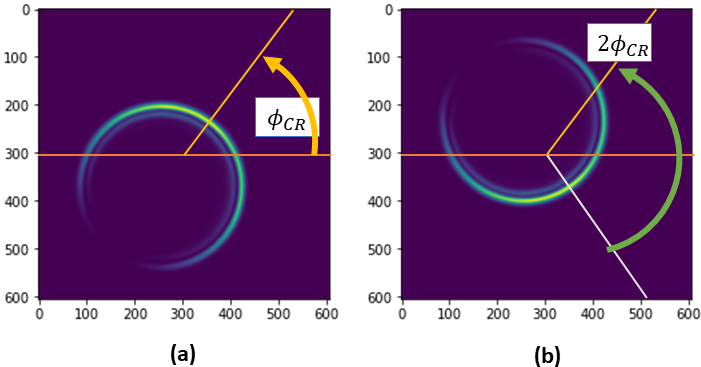
\includegraphics[width=0.65\linewidth]{rot.PNG}
    \caption{(a) Experimental crescent ring image indicating $\phi_{CR}$. (b) The image in (a) mirror flipped in the axis crossing the gravicenter. A $2\phi_{CR}$ rotation should make it almost equal to (a). Note that what we end up comparing at that angle is each half along the main axis, where they should be symmetric. }
    \label{fig:kalk}
\end{figure}

\begin{algorithm}
\caption{\rule{0pt}{3.5mm}{} {\bf The Kalkandjiev-Rotation Algorithm} - High Level Pseudo-Code. \newline To get $\Delta \Phi_{LP}$ use $I\in\{I_{pb},I_{ref}\}$, to get $\phi_{CR_{pb}}$, $\phi_{CR_{ref}}$ then $\Delta\Phi_{LP}=(\phi_{CR_{pb}}-\phi_{CR_{ref}})/2$.}\label{alg:rot}
\func{ $C(\ phi;\ I,\ I_{mirror\ x},\ \vec{g}_{grav},\ $ similarity $(\cdot,\cdot))$}{
	$rot \gets $affine rotation$(\ I_{mirror\ x},\ $angle$=phi,\ $rotation\_center$=\vec{g}_{grav})$\;
	{\bf return} -similarity($rot,I$)\\
}
\vspace{0.2cm}
\Given{ $I,\ C,\ I,\ \vec{g}_{grav},\ similarity(\cdot,\cdot),\  \phi_{min}:=-\pi,\ \phi_{max}:=\pi$}{\vspace{0.1cm}
$I\gets$ iX standard $(I)$\;
$I_{mirror}\gets$ x axis mirror $I$ at $y=\vec{g}_{grav}[0]$\;
$w\gets \{I,\ I_{mirror},\ \vec{g}_{grav},\ $similarity$(\cdot,\cdot)\}$\;
$x\gets$ 1D minimum Search $(C(\cdot;w),\ \phi_{min},\ \phi_{max})$\;
$\phi_{CR}\gets$ get angle to crest hill with alg. \ref{alg:toMax} $(\ x/2\ )$\;
{\bf return} (take to $(-\pi,\pi)$ with alg. \ref{alg:topipi} $\{\phi_{CR}\}$)\DontPrintSemicolon{\Comment*[r]{It returns $ \phi_{CR}$}}\vspace{0.1cm}
}
\end{algorithm}

A problem this algorithm (as well as some of the next ones) presents is that the obtained optimal relative rotation can equally likely turn out to be $\phi_{CR}$ (the angle to the crest's hill), or the angle to where the minimum intensity should be (the valley of the crest), which is $\pi$ rad apart from $\phi_{CR}$. Then, to obtain the correct value of $\Delta\Phi_{LP}$, we need to compute the difference employing for both rather $\phi_{CR}$ or $\phi_{CR}\pm\pi$. Therefore, once we have obtained the angle $\varphi$, which can be anyone in $\{\phi_{CR},\ \phi_{CR}+\pi\}$, we need a post-process to distill say, $\phi_{CR}$. We do this employing Algorithm \ref{alg:toMax}. Essentially, the trick is to notice that which-ever is $\varphi$, it equally indicates the main symmetry axis. Thus, its orthogonal axis can be described by $\varphi+\pi/2$, whichever it was in $\{\phi_{CR},\phi_{CR}+\pi\}$. This orthogonal axis to the main symmetry axis is $y=g_y+tan(\varphi+\pi/2)(x-g_x)$, where $(g_x,g_y)=\vec{g}_{grav}$. Knowing this, we can define an index mask that indicates which indices of the image are above the line and which ones are below the line. With it, we add up the pixel intensities for the ones laying above and the ones laying below the asymmetric axis and compute their difference (up minus down) $\Delta ring$. If the difference is positive, then the ring maximum is above this axis and $\phi_{CR}$ lays in $(0,\pi)$, else, it will be in $(-\pi,0)$.

\begin{algorithm}
\caption{\rule{0pt}{3mm}{} Knowing {\bf $\varphi \in\{\phi_{CR},\phi_{CR}-\pi\}$ obtain $\phi_{CR}$} - High Level Pseudocode}\label{alg:toMax}
{\small 
\Given{$\varphi,\ I,\ \vec{g}_{grav}$ :}{
\uIf{$\varphi==0\ or\ abs(\varphi)==\pi$}{
$\varphi\gets \varphi+10^{-12}$ \Comment*[r]{\small Not ideal, but will never get such a good precision}
}
$\Delta ring\gets$ given orthog. axis ang. to main ax. get $I$ diff. at each side$(\varphi+\pi/2,\ I,\ \vec{g}_{grav})$\;
\uIf{$\Delta ring>0$\vspace{-0.3cm}}{
\DontPrintSemicolon{\CommentMath*[r]{$\phi_{CR}$ is the one in (0,pi)}}
\uIf{$\varphi<0$}{{\bf return }$\varphi+\pi$}
\uElse{{\bf return} $\varphi$}
}
\uElse{
\uIf{$\varphi>0$}{{\bf return }$\varphi-\pi$}
\uElse{{\bf return} $\varphi$}\vspace{0.1cm}
}
}}
\end{algorithm}\vspace{-0.25cm}

\subsection*{B.6.4. The Mirror Flip Algorithm}\vspace{-0.15cm}
This is another algorithm that exploits the supposed self-symmetry of the crescent ring along its main axis (geometric property (a)). Using affine operation \eqref{mirror}, we can compute the result of taking a mirror flip of an image along an arbitrary axis crossing the point $(c_x,c_y)$ at an angle $\theta$. Then, since the crescent rings are symmetric along their main axis, which is the axis crossing the gravicenter $\vec{g}_{grav}$ (known) and oriented at an angle $\phi_{CR}$, we can 1D search for the angle at which to apply the mirror flip such that the result is most similar to the original image (this time the minimum is bounded in $[-\pi/2,\pi/2)$, since we look for an axis). The followed procedure is described in Algorithm \ref{alg:mirror}. This algorithm as well, only provides us $\phi_{CR}$ up to $\pi$, so it requires the post-processing technique of Algorithm \ref{alg:toMax}.

\begin{algorithm}
\caption{ \rule{0pt}{3.5mm}{} {\bf The Mirror Flip Algorithm} - High Level Pseudo-Code\newline To get $\Delta \Phi_{LP}$ use $I\in\{I_{pb},I_{ref}\}$, to get $\phi_{CR_{pb}}$, $\phi_{CR_{ref}}$ then $\Delta\Phi_{LP}=(\phi_{CR_{pb}}-\phi_{CR_{ref}})/2$.}\label{alg:mirror}
\func{ $C(\ phi;\ I, \vec{g}_{grav},\ $ similarity $(\cdot,\cdot))$}{
	$mirror \gets $affine mirror flip on custom axis$(\ I,\ $at angle$=phi,\ $axis\_center$=\vec{g}_{grav})$\;
	{\bf return} -similarity($mirror,I$)\\
}
\vspace{0.2cm}
\Given{ $I,\ C,\ I,\ \vec{g}_{grav},\ similarity(\cdot,\cdot),\  \phi_{min}:=-\frac{\pi}{2},\ \phi_{max}:=\frac{\pi}{2}$}{\vspace{0.1cm}
$I\gets$ iX standard $(I)$\;
$w\gets \{I,\ \vec{g}_{grav},\ $similarity$(\cdot,\cdot)\}$\;
$x\gets$ 1D minimum Search $(\ C(\cdot;w),\ \phi_{min},\ \phi_{max}\ )$\;
$\phi_{CR}\gets$ get angle to crest hill with alg. \ref{alg:toMax} $(\ x/2\ )$\;
{\bf return} (take to $(-\pi,\pi)$ with alg. \ref{alg:topipi} $\{\phi_{CR}\}$)\DontPrintSemicolon{\Comment*[r]{It returns $ \phi_{CR}$}}\vspace{0.1cm}}
\end{algorithm}\vspace{-0.3cm}



\subsection*{B.6.5. The Gravicenter Regression Algorithm}\vspace{-0.15cm}
This is an improvement of another idea suggested by Prof. Kalkandjiev. Let us take a circular mask of radius $r$ around the gravicenter $\vec{g}$ and erase the pixels outside the circle. The gravicenter of the masked image, $\vec{g}_r$, will land in a different spot as a function of the radius of the mask. If the radius is so small that no pixel with ring information is inside, the gravicenter will lay in the center of the image, where the whole image gravicenter was $\vec{g}\simeq\vec{g}_r$ (assuming the image is iX standardized). If we make the circle so big as to include the whole crescent ring, then the mask-gravicenter will lay again around the gravicenter of the whole image $\vec{g}\simeq\vec{g}_r$. However, for intermediate radii the gravicenter will land in different spots, all theoretically within the main symmetry axis. This is because the circle always takes a symmetric piece of each half of the ring within it. Because $\vec{g}$ is tilted towards the maximum intensity of the crescent ring, as $r$ increases the mask will first intersect only with the side of maximum intensity. Therefore, $\vec{g}_r$ will get even closer to that side of the ring than $\vec{g}$. It will keep approaching as $r$ increases, until at a certain $r_0$, the circle mask intersects with enough of the other side of the ring, to make $\vec{g}_r$ move back towards $\vec{g}$. It turns out the $r_0$ point lays exactly in the Poggendorff dark ring for a ring with big enough $\rho_0$. 

The magnificent idea proposed by Prof. Kalkandjiev was that we could take the point $\vec{g}_{r0}=(g_x^{(r0)}, g_y^{(r0)})$, which is the furthest one from $\vec{g}=(g_x,g_y)$, to compute their relative vector $\vec{G}:=\vec{g}_{r0}-\vec{g}$, which will have a magnitude $r_0$ and an angle $\phi_{CR}$, because all $\vec{g}_r$ lay along the main axis\footnote{He called this vector $\vec{G}$ the {\em gradient vector}, because it somehow points in the direction of steepest intensity surface increase. Thus the original name of the algorithm was {\em the Gradient algorithm}.}. Then not only we get directly $\phi_{CR}=tan^{-1}\qty(\frac{g_y^{(r0)}-g_y}{g_x^{(r0)}-g_x})$, but we know $r_0$, the distance from the gravicenter to the Poggendorff dark ring along the main axis. He suggested that this should be related by a simple relation with the distance to the geometric center $R_0$ along the same axis, which if found, $R_0(r_0)$ would provide us an estimate of the geometrical center $\vec{g}_{geom}$. At the same time, this would give us access to more advanced algorithms to refine $\phi_{CR}$.

However, it turns out there is not a trivial relation between $R_0$ and $r_0$ if we allow $w_0,R_0,z$ to vary. This means, we could train a function to predict $R_0(r_0)$, but then we would loose the elegance of the method. In addition, yes, it is true that to compute $\vec{G}$, $\vec{g}_{r0}$ is the most convenient one of the $\vec{g}_r$: since it is the furthest one form $\vec{g}$, it is the one that the same perturbation in position will affect the least to the indicated angle $\phi_{CR}$. Nevertheless, it could happen that precisely at radious $r_0$ the circle starts to take in very noisy parts of the ring. Why then not use just the previous $r$-s? Well, because it could happen that it is the inner part that is noisier. Then why not wait for the mask to take as much of the ring as possible to compensate the noise?

Following this criticism, we can give a more holistic version of the algorithm. We can use all the $\vec{g}_r$, each of which is an estimate of a point on the main axis, to fit a line by a least squares or a RANSAC \cite{RANSAC} method. From the fitted line $y=a+bx$, which should represent the main symmetry axis, we can compute $\phi_{CR}$ up to $\pi$ with $tan^{-1}(b)$. Then, Algorithm \ref{alg:toMax} would end up deciding $\phi_{CR}$. The approach is summarized in Algorithm \ref{alg:gradient}.

\begin{figure}[h!] 
     \centering 
    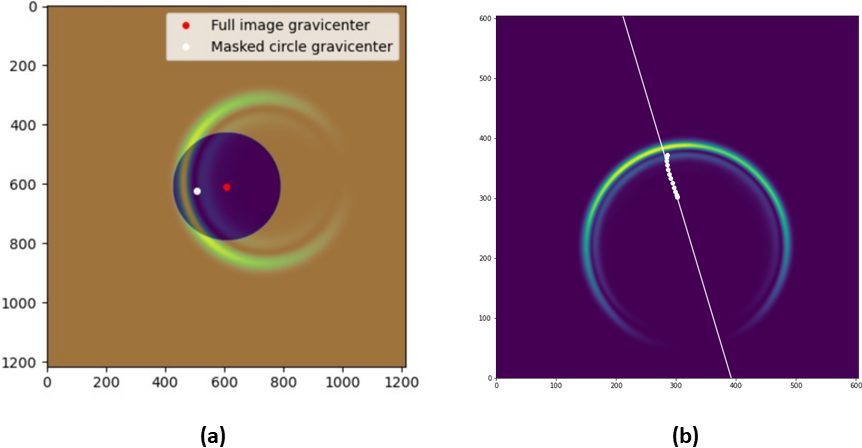
\includegraphics[width=0.72\linewidth]{grad.PNG}
    \caption{(a) A problem experimental crescent ring with the $r_0$ mask over it. The $\vec{G}$ vector is the one joining the two gravicenters. (b) Another experimental image, showing all the $\vec{g}_r$ as white dots. The white line is the linear fit estimating the main axis obtained with them.}
    \label{fig:grav}
\end{figure}

\begin{algorithm}
\caption{ \rule{0pt}{3.5mm}{} {\bf The Gravicenter Regression Algorithm} - High Level Pseudo-code\newline To get $\Delta \Phi_{LP}$ use $I\in\{I_{pb},I_{ref}\}$, to get $\phi_{CR_{pb}}$, $\phi_{CR_{ref}}$ then $\Delta\Phi_{LP}=(\phi_{CR_{pb}}-\phi_{CR_{ref}})/2$.}\label{alg:gradient}
{\small 
\Given{$I,\ \vec{g}_{grav},\ N_r,\ r_{min},\ r_{max}$ :}{
$r_s\gets$ equispaced grid of $N_r$ points in $[r_{min},r_{max}]$\;
$\mathfrak{r}(x,y)\gets$ array giving the radial distance from $(x,y)$ in $I(x,y)$ to $\vec{g}_{grav}$\;
$\vec{g}_rs\gets$ empty [$N_r$+1, 2] matrix of floats\;
\For{$k\ \in\ \{0,1,...,N_r-1\}$}{
$\vec{g}_rs[k,:]\gets$ compute gravicenter $(\ I[\ \mathfrak{r}(x,y)<r_s[k]\ ]\ )$\;
}
$\vec{g}_rs[-1,:]=\vec{g}_{grav}$\;
$a,b\gets$ {\small least square or RANSAC fit $y=a+bx$ to observed $\{(x_k,y_k)\}_k=\{\vec{g}_rs[k,1],\ \vec{g}_rs[k,0]\}_k$\;
$\varphi\gets$ tan$^{-1}(b)$}\;
$\phi_{CR}\gets$ get angle to crest hill with alg. \ref{alg:toMax} ( $\varphi$ )\;
{\bf return} (take to $(-\pi,\pi)$ with alg. \ref{alg:topipi} $\{\phi_{CR}\}$)\DontPrintSemicolon{\Comment*[r]{It returns $ \phi_{CR}$}}\vspace{0.1cm}}
}
\end{algorithm}\vspace{-0.15cm}

\subsection*{B.6.6. The Bimodal Histogram Algorithm}\vspace{-0.15cm}
We do not have an analytic expression for the angular distribution of the intensity if we center the polar node in the gravicenter $\mathcal{I}(\theta;\vec{g}_{grav})$. For the geometric center we do have it: by equation \eqref{cosine}, it is a squared cosine. Yet, since the gravicenter is tilted towards the maximum intensity spot along the main axis and the ring should be symmetric about such an axis, the angular profile about the gravicenter still has an interesting shape. It looks like a symmetric bimodal distribution. There are two hills that symmetrically get close to each other with a slight depression exactly in the maximum intensity angular spot and a deep valley reaching 0 intensity in the minimum intensity angular spot. See Figure \ref{fig:histo}. This makes $\mathcal{I}(\theta,\vec{g}_{grav})$ a periodic function if $\theta\in\R$, with two symmetry points within each period: one will indicate $\phi_{CR}$, the other one $\phi_{CR}\pm\pi$.

We could then calculate the image in polar coordinates, centered in the gravicenter, integrate the radial part and get the angular profile $\mathcal{I}(\theta,\vec{g}_{grav})$. Finally, looking for the point offering biggest symmetry could work to get $\phi_{CR}$ up to $\pi$. Yet, this is a poorer version of say the Mirror flip algorithm, since we loose detail of the radial part, which could be critical in the matching. In addition we relay completely in the strict symmetry property around a single point.

A more holistic algorithm perhaps, is to only assume that the angular histogram $\mathcal{I}(\theta,\vec{g}_{grav})$ represents the density of two modes, which need not have the same standard deviation properties, but such that there is a particular angle $\phi_{CR}$ for which they are best separated. This could be measured by the average intra-mode variance. Given a boundary $t$ and considering the angular nodes $\{\theta_k\}_{k=0}^{N_\theta}$, we define the mean and variance of each mode as:\vspace{-0.15cm}
\begin{equation}
\mu_1(t) = \frac{1}{\sum_{k=0}^{k:\theta_k=t}\mathcal{I}(\theta_k; \vec{g}_{grav})}\sum_{k=0}^{k\ :\ \theta_k=t} \theta_k\mathcal{I}(\theta_k; \vec{g}_{grav})\quad  \quad \mu_2(t) = \frac{1}{\sum_{k\ :\ \theta_k=t}^{N_{\theta}}\mathcal{I}(\theta_k; \vec{g}_{grav})}\sum_{k\ :\ \theta_k=t}^{N_{\theta}} \theta_k\mathcal{I}(\theta_k; \vec{g}_{grav})
\end{equation}
\begin{equation}
\small
var_1(t)= \frac{\sum_{k=0}^{k\ :\ \theta_k=t} (\theta_k-\mu_1)^2\mathcal{I}(\theta_k; \vec{g}_{grav})}{\sum_{k=0}^{k:\theta_k=t}\mathcal{I}(\theta_k; \vec{g}_{grav})}\quad  \quad \quad var_2(t) = \frac{\sum_{k\ :\ \theta_k=t}^{N_{\theta}} (\theta_k-\mu_2)^2\mathcal{I}(\theta_k; \vec{g}_{grav})}{\sum_{k\ :\ \theta_k=t}^{N_{\theta}}\mathcal{I}(\theta_k; \vec{g}_{grav})}
\end{equation}
Then, we can define an average intra-mode variance, following the Otsu intra-class variance \cite{Otsu}, as:
\begin{equation}\label{intra}
\small
var(t) = \frac{\sum_{k=0}^{k:\theta_k=t}\mathcal{I}(\theta_k; \vec{g}_{grav})}{\sum_{k=0}^{N_{\theta}}\mathcal{I}(\theta_k; \vec{g}_{grav})}\ var_1(t)+\frac{\sum_{k:\theta_k=t}^{N_{\theta}}\mathcal{I}(\theta_k; \vec{g}_{grav})}{\sum_{k=0}^{N_{\theta}}\mathcal{I}(\theta_k; \vec{g}_{grav})}\ var_2(t)
\end{equation}
The scheme would then be to look for the boundary angle $t$ separating the modes that minimizes the average intra-mode variance \eqref{intra}. This is resilient to asymmetrically noisy crests assuming that the gravicenter (about which we compute the angular histogram) is still aligned with the geometric center at $\phi_{CR}$. The method is isomorphic to the Otsu algorithm \cite{Otsu} employed to find the optimal binarization threshold in images that are assumed to have a bimodal histogram.

We realize however that yet an additional consideration must be taken. The angular histogram plots are only computed for a single fixed period $\theta\in[-\pi,\pi]$ in a finite array. As can be seen in Figure \ref{fig:histo}, this means that as a function of which was $\phi_{CR}$, we will have our ideal plot where to apply the algorithm shifted. We can solve this as follows: each $s$ shifted version of the histogram will have its own minimum intra-class variance threshold $t^*(s)$. This optimal threshold will have the minimum intra-class variance when the histogram is exactly shifted by an angle $s^*\in\{\phi_{CR},\phi_{CR}\pm\pi\}$, leaving a symmetric histogram plot. In fact, in that moment, $t^*$ will also indicate the main axis $t^*(s^*)\in\{\phi_{CR},\phi_{CR}\pm\pi\}$. Therefore, we have a nested 1D optimization problem by which we look for the histogram shift $s$ that gives the optimal threshold $t^*(s)$ of minimum intra-class variance. Then the shift for the minimum $s^*$ and the minimum variance threshold within it $t^*(s^*)$, should both yield $\phi_{CR}$ (up to $\pi$).
\begin{figure}[h!] 
     \centering 
    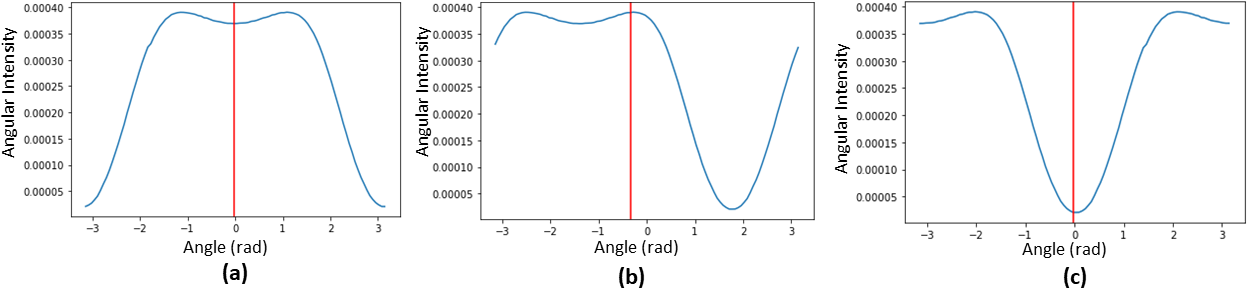
\includegraphics[width=0.98\linewidth]{bimod.PNG}
    \caption{ Angular histograms with the gravicenter as polar center. They show a red line indicating the minimum intra-mode variance threshold. They are shifted versions of the histogram of a same image. (a) and (c) show the shifts offering the minimum minimum intra-mode variance, while (b) shows an intermediate one. Note that in the optimal shifts, the optimal thresholds will always be found around the middle of the plot. When tracing back this angle by the shift, it will give $\phi_{CR}$ up to $\pi$. The shift itself should also give $\phi_{CR}$ up to $\pi$.}
    \label{fig:histo}\vspace{-0.35cm}
\end{figure}

\begin{algorithm}
\caption{ \rule{0pt}{3.5mm}{} {\bf The Bimodal Histogram Algorithm} - High Level  Python Pseudo-code \newline To get $\Delta \Phi_{LP}$ use $I\in\{I_{pb},I_{ref}\}$, to get $\phi_{CR_{pb}}$, $\phi_{CR_{ref}}$ then $\Delta\Phi_{LP}=(\phi_{CR_{pb}}-\phi_{CR_{ref}})/2$.}\label{alg:histo}
{\small 
\func{$get\ min\ variance\ theshold\ (\vec{h}, \vec{\theta}s)$:}{
$w1\gets $ cumulative sum $(\ \vec{h}\ )$\Comment*[r]{\small returns a vector: entry $k$ is $\sum_{j=0}^k\vec{h}[j]$}
$w2\gets $ flip order ( cumulative sum $(\ $ flip order $(\vec{h})$ $\ )$ )\;
$\vec{\mu_1}s\gets $ cumulative sum ( $\vec{h}*\vec{\theta}s$ ) $/w1$\Comment*[r]{\small prod. $*$ and div. $/$ are element-wise}
$\vec{\mu_2}s\gets $ flip order ( cumulative sum( flip order($\vec{h}*\vec{\theta}s$) )$/w2$ )\;

$vars\gets\ w1[:-1]*w2[1:]\ *(\vec{\mu_1}s[:-1]-\vec{\mu_2}s[1:])^2$\;
$k_{min}\gets\ $argmin$(vars)$\;
{\bf return }$\vec{\theta}s[k_{min}],\ vars[k_{min}]$\Comment*[r]{\small returns min var threshold angle $t^{*}$ and $var(t^{*})$}\vspace{0.11cm}
}
\Given{$I,\ \vec{g}_{grav},\ N_\theta\ N_r:$}{
$I_{polar}\gets$ to polar coordinates($I,\ \vec{g},\ N_\theta,\ N_r$) \Comment*[r]{$N_\theta$ angular pts $N_r$ radial pts}
$\vec{h}\gets $ sum components along $r$'s axis ($I_{polar}$) \Comment*[r]{\small angular histogram about $\vec{g}$}
$\vec{\theta}s\gets $ integers array ($0,1,...,\ N_\theta-1$)\;
$t_{opt}s,\ var_{opt}s\gets $ two empty arrays of length $s_{max}-s_{min}$\;
\For{$k\ \in\ \{0,1,..., s_{max}-s_{min}-1\}$}{
$\vec{h}_{shifted}\gets $ concatenate ($\vec{h}[s_{min}+k:],\vec{h}[:s_{min}+k]$)\;
$t_{opt}s[k],var_{opt}s[k]\gets$ get min variance threshold $(\vec{h}_{shifted}, \vec{\theta}s)$\;
}
$k_{min}\gets $ argmin$(var_{opt}s)$\;
$min\_var\_t\_shifted \gets t_{opt}s[k_{min}]$\Comment*[r]{\small $t^*$ of min $var(t^*)$ but for shifted frame}
$min\_var\_shift\gets\ k_{min} +\ s_{min}$\Comment*[r]{\small the shift in $\vec{h}$ to get min $var(t^{*})$}
$aux\gets\ (\ min\_var\_t\_shifted//(N_\theta-min\_var\_shift) \ )\ >\ 0$\Comment*[r]{\small $//$ is integer division}
$min\_var\_t\gets min\_var\_t\_shifted+min\_var\_shift-N_\theta\cdot aux $\Comment*[r]{\small $t^*$ of min $var(t^*)$}

$\phi_{{CR}_1}\gets min\_var\_t \cdot 2\pi/N_\theta$\;
$\phi_{{CR}_2}\gets min\_var\_shift \cdot 2\pi/N_\theta$\Comment*[r]{\small this should also be $\phi_{CR}$, but $\phi_{CR1}$ is bettter}
{\bf return } (take to $(-\pi,\pi)$ with alg. \ref{alg:topipi} $\{\phi_{CR_1}\}$)\DontPrintSemicolon{\Comment*[r]{It returns $ \phi_{CR}$}}\vspace{0.1cm}

}}
\end{algorithm}
The implemented scheme is described in Algorithm \ref{alg:histo}. Following it, we first run a gross search for an estimate of the optimum shift $s^*$ and then zoom-in around it to perform a brute-force search of the actual optimum. It was done this way instead of using a nested 1D optimization, for each brute force minimum variance search $t^*(s)$ was found to be easily vectorizable (see the function in Algorithm \ref{alg:histo}).\vspace{-0.2cm}

\subsection*{B.6.7. The Blazquez Algorithm}\vspace{-0.1cm}
The following algorithm was thought by Carles Blazquez, a good classmate and a great physicist. Let us define $J(x,y)$ as the crescent ring image pixel-wise added with a $\pi$ rad rotated version of itself: $J(x,y):=I(x,y)+Rot\_\pi\_about\_\vec{g}\ [\ I(x,y)\ ]$. Then, the essential idea behind the algorithm is that if we rotate $J(x,y)$ by $\pi/2$ rad, the resulting image will be exactly the same as $J(x,y)$ only if the rotation center $\vec{g}$ was chosen to be the geometric center of the ring $\vec{g}_{geom}$. This is because by the symmetry (d) in the list in (B.1), adding a crescent ring image and its $\pi$ rotated version about $\vec{g}_{geom}$, we get the hollow ring we would have got if the input was CP. Then, this hollow ring of constant angular profile will naturally be the same as its $\pi/2$ rotated version, and actually any other rotation of itself. See Figure \ref{fig:blaz}.

If we only looked for $J(x,y)$ directly being a hollow uniform ring, we would be asking the ring to be symmetric with respect to the main axis, just like with the Mirror algorithm. However, the Blazquez algorithm is more general since when we ask it to be at the same time equal to the $\pi/2$ rotated version, we are pair-wise comparing each pair of fourth parts of the ring (see Figure \ref{fig:blaz}). Thus it will be robuster to noise that breaks the strict symmetry about the main axis.

\begin{figure}[h!] 
     \centering 
    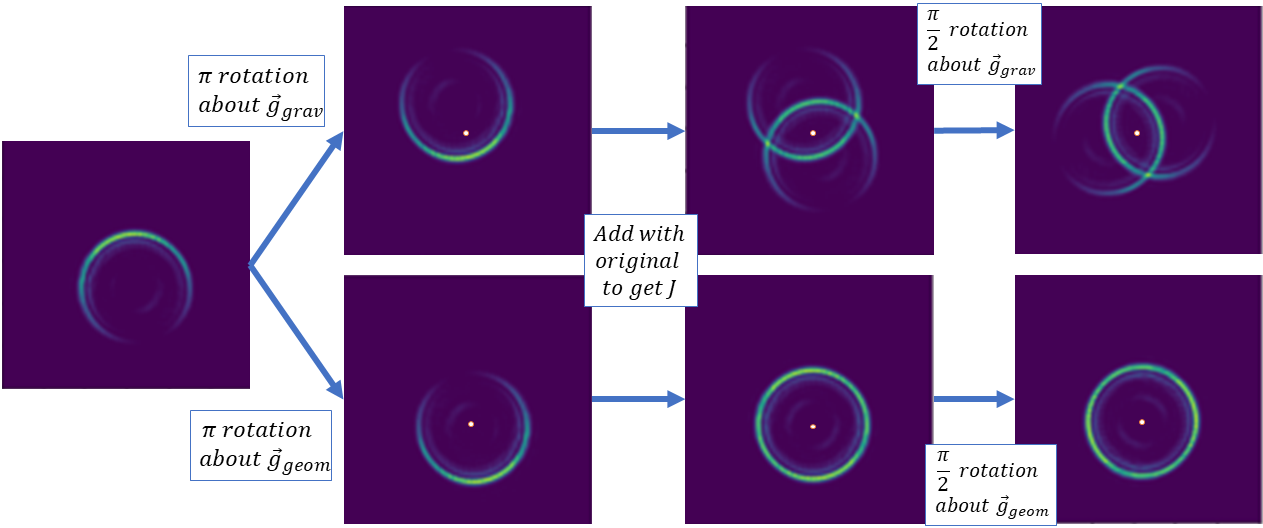
\includegraphics[width=0.9\linewidth]{blaz.PNG}
    \caption{ Schematic depiction of the construction of $J$ choosing $\vec{g}_{grav}$ or $\vec{g}_{geom}$ as rotation centers. }
    \label{fig:blaz}
\end{figure}

\begin{algorithm}
\caption{ \rule{0pt}{3.5mm}{} {\bf The Blazquez Algorithm } - High Level Pseudo-code\newline To get $\Delta \Phi_{LP}$ use $I\in\{I_{pb},I_{ref}\}$, to get $\phi_{CR_{pb}}$, $\phi_{CR_{ref}}$ then $\Delta\Phi_{LP}=(\phi_{CR_{pb}}-\phi_{CR_{ref}})/2$.}\label{alg:Blaz}
\func{$C_{Blz}(\ c_x,\ c_y;\ I,\  similarity(\cdot,\ \cdot)\ ): $\DontPrintSemicolon{\Comment*[r]{\small MAE \eqref{MAE} good similarity for this}}\vspace{-0.5cm}}{
$J\gets\ I\ +$ rotate $\pi$ around $(\ I,\ (c_x,\ c_y)\ )$\;
{\bf return } -similarity( $J$, rotate $\pi/2$ around ( $J,\ (c_x,\ c_y)$ ) }

\Given{$I,\ \vec{g}_{grav},\ similarity(\cdot,\cdot)\ :$}{
$w\gets\{\ I,\ similarity(\cdot,\ \cdot)\ \} $\;
$\vec{g}_{geom}\gets$ 2D min. Search $(\ C_{Blz}(\cdot,\cdot;w),\ (c_{x\; min},c_{x\; max})=(0,\; width(I)),\ (c_{y\; min},c_{y\; max})=(0,\; height(I))\ )$\; 
$(G_x,G_y)\gets\vec{g}_{grav}-\vec{g}_{geom}$\;
$\phi_{CR}\gets$ tan$^{-1}(G_y/G_x)$\;
{\bf return } (take to $(-\pi,\pi)$ with alg. \ref{alg:topipi} $\{\phi_{CR}\}$)\DontPrintSemicolon{\Comment*[r]{It returns $ \phi_{CR}$}}\vspace{0.1cm}}
\end{algorithm}


In fact, perhaps the most precise of the algorithms in the work could be a variant of Blazquez's algorithm, in which the minimized metric in the 2D search for $\vec{g}_{geom}$ is not the difference between $J(x,y)$ and the $\pi/2$ rotated $J$, but the differences between $J$ and a range of $\theta_k$ rotations of $J$. Each additional angle $\theta_k$ we added would make the algorithm each time more holistic, allowing to absorb noises in the crests of the generated hollow ring when the rotations are made about $\vec{g}_{geom}$. This algorithm however is left as a future work if Blazquez's algorithm turns out to perform well.

The current implementation, following Blazquez's original idea is listed in Algorithm \ref{alg:Blaz}. One thing is left yet. What we obtain with the algorithm so far, is the geometric center $\vec{g}_{geom}$. Then the trivial way to obtain $\phi_{CR}$ from it is by using that the gravicenter $\vec{g}_{grav}$ is aligned with the geometric center along the main axis. By computing the relative vector along the axis $\vec{G}=(G_x,G_y):=\vec{g}_{grav}-\vec{g}_{geom}$ we could then get $\phi_{CR}=tan^{-1}(G_y/G_x)$.\vspace{-0.2cm}


\subsection*{B.6.8. The Squared Cosine Fit Algorithm}\vspace{-0.1cm}
This is another algorithm to look for the geometric center and in the way find $\phi_{CR}$. We know that the angular histogram of a CR crescent ring image will only have a cosine squared shape given by equation \eqref{cosine} when the angular intensity profile $\mathcal{I}(\theta;\vec{c})$ is computed using as polar center $\vec{c}=(c_x,c_y)$ the geometrical center of the ring $\vec{g}_{geom}$. We can parameterize this cosine square following \eqref{cosine} as:\vspace{-0.1cm}
\begin{equation}
\mathcal{I}(\theta;\vec{c}=\vec{g}_{geom}, C,\Phi_{LP})=K+Ccos^2(\theta/2-\Phi_{LP})\vspace{-0.1cm}
\end{equation}
where we included an additional degree of freedom $K\in\R$ to account for baseline noise.

This means we could make a 2D search in the possible polar center space $\vec{c}\in\Omega$ computing angular histograms at each point and fitting a cosine square of parameters $K,C,\Phi_{LP}$ until the fitting error is minimum. Alternatively the followed approach could be to make a 4D search in the whole $\vec{c},K,C,\Phi_{LP}$ space. However, the least square error cosine square fit can be done "exactly" within each $\vec{c}$ employing the normal equations. To do this, we first use the identity $cos^2(x)=(1+cos(2x))/2$ and then the relation employed in (A.1.1) to write a de-phased cosine as a sum of a sine and a cosine, to get:\vspace{-0.1cm}
\begin{equation}
K+Ccos^2(\theta/2-\Phi_{LP})=E+Acos(\theta)+Bsin(\theta)\vspace{-0.1cm}
\end{equation}
with $C/2=\sqrt{A^2+B^2}$,  $\Phi_{LP}=tan^{-1}(B/A)$ and $K+C/2=E$. 


\mybox{Given $\vec{c}\in\R^2$, we compute the angular histogram for the angle bins $\{\theta_k\}_{k=1}^{N_\theta}$ to be $\{\mathcal{I}_k\}_{k=1}^{N_\theta}$. Then, we can impose the fit with the $N_\theta$ equations of real unknowns $E,A,B$:
\begin{equation}
\small
\hspace*{-0.5cm}
\begin{cases}
\mathcal{I}_1=E+Acos(\theta_1)+Bsin(\theta_1)\\
\cdots\\
\mathcal{I}_{N\theta}=E+Acos(\theta_{N\theta})+Bsin(\theta_{N\theta})
\end{cases}\hspace*{-0.5cm}\Rightarrow
\begin{pmatrix}
\mathcal{I}_1\\
\vdots\\
\mathcal{I}_{N\theta}
\end{pmatrix}=\begin{pmatrix}
1 & cos(\theta_1) & sin(\theta_1)\\
\vdots&\vdots&\vdots\\
1 & cos(\theta_{N\theta}) & sin(\theta_{N\theta})
\end{pmatrix}\begin{pmatrix}
E\\
A\\
B
\end{pmatrix}\Leftrightarrow \vec{\mathcal{I}}=\pmb{H}\vec{x}
\end{equation}
The vector $\pmb{H}\vec{x}\in\R^{N_\theta}$ is a linear combination of the three column vectors of $\pmb{H}$ with coefficients $\vec{x}=(E,A,B)\in\R^3$. Then, to find a solution of the system is to get the coefficients for the combination to give the vector $\vec{\mathcal{I}}=(\mathcal{I}_1,...,\mathcal{I}_{N_\theta})\in\R^{N_\theta}$. For noisy images or general $\vec{c}\neq \vec{g}_{geom}$, the $\R^{N_\theta}$ vector $\vec{\mathcal{I}}$ need not lay in the 3 dimensional subspace spanned by these 3 vectors. Let us call it, the subspace $\mathcal{H}$. This means that in general, no such linear combination exists. Still, we can look for the closest possible linear combination $\pmb{H}\vec{x}$ (in terms of Euclidean norm) to $\vec{\mathcal{I}}$. Geometrically (and by the Hilbert projection theorem), this is given by the orthogonal projection of $\vec{\mathcal{I}}$ into $\mathcal{H}$. If $\vec{x}_{opt}$ gives this linear combination, then $\pmb{H}\vec{x}_{opt}$ will be orthogonal to $\vec{\mathcal{I}}-\pmb{H}\vec{x}_{opt}$. That is, their scalar product will be zero: $\vec{x}_{opt}^t\pmb{H}^{t}(\vec{\mathcal{I}}-\pmb{H}\vec{x}_{opt})=0\Leftrightarrow \vec{x}_{opt}^t(\pmb{H}^t\vec{\mathcal{I}}-\pmb{H}^t\pmb{H}\vec{x}_{opt})=0$. This has a non-trivial solution if $\pmb{H}^t\vec{\mathcal{I}}=\pmb{H}^t\pmb{H}\vec{x}_{opt}$. \vspace{0.15cm}

Now, because the columns of $\pmb{H}$ are linearly independent, their linear combination will be $\vec{0}$, $\pmb{H}\vec{x}=\vec{0}$, only if $\vec{x}=\vec{0}$. The kernel of $\pmb{H}$ is thus $\{\vec{0}\}$. Then, since $\pmb{H}^t\pmb{H}=\vec{0}\Rightarrow \vec{x}^t\pmb{H}^t\pmb{H}=0\Rightarrow |\pmb{H}\vec{x}|^2=0\Rightarrow \pmb{H}\vec{x}=\vec{0}$, the kernel of $\pmb{H}$ and $\pmb{H}^t\pmb{H}$ are the same. Therefore $\pmb{H}^t\pmb{H}$ being a square}
\mybox{ matrix with kernel $\{\vec{0}\}$, it is invertible, and we can get the solution coefficients as $\vec{x}_{opt}=(\pmb{H}^t\pmb{H})^{-1}\pmb{H}^t\vec{\mathcal{I}}$. This is the well known least squares or normal equation method that can be found in many text books, like in Ref. \cite{leastsquares}.\vspace{0.15cm}

To see why it is called this way, observe that the vector $\vec{\mathcal{I}}-\pmb{H}\vec{x}$ is the error vector between the observed points and the predicted ones by the fit. Its norm squared will give us the sum of squared errors for the fit. Additionally, $\vec{\mathcal{I}}-\pmb{H}\vec{x}$ is geometrically the vector joining the combination $\pmb{H}\vec{x}$ restricted in $\mathcal{H}$, with $\vec{\mathcal{I}}$. Its magnitude is then minimum when it is orthogonal to $H$. Thus, $\vec{x}_{opt}=(\pmb{H}^t\pmb{H})^{-1}\pmb{H}^t\vec{\mathcal{I}}$ gives the least square error fit. 
}
If we build a cost function to give as a function of $\vec{c}$ (the polar center of the angular plot), the fit error of the least-square-error cosine square fit, the cost will be minimum when $\vec{c}=\vec{g}_{geom}$. Then, once we know $A,B$ for $\vec{c}=\vec{g}_{geom}$ we can immediately obtain $\Phi_{LP}$ as $\Phi_{LP}=tan^{-1}(B/A)$. We implemented it following Algorithm \ref{alg:cosFit}.

\begin{algorithm}
\caption{\rule{0pt}{3.5mm}{} {\bf The Squared Cosine Fit Algorithm} - High Level Pseudo-Code \newline To get $\Delta \Phi_{LP}$ use $I\in\{I_{pb},I_{ref}\}$, to get $\Phi_{LP_{pb}}$, $\Phi_{LP_{ref}}$ then $\Delta\Phi_{LP}=\Phi_{LP_{pb}}-\Phi_{LP_{ref}}$. }\label{alg:cosFit}
\func{$C_{csf}(\ c_x,\ c_y;\ I,\ \vec{\theta}_s,\ N_\theta,\ N_r, \ er \ )$}{
$I_{polar} \gets $ to polar coordinates $(I,(c_x,c_y), N_\theta, N_r)$\Comment*[r]{$N_\theta$ angular pts $N_r$ radial pts}
$\vec{\mathcal{I}}\gets $ sum components along $r$'s axis ($I_{polar}$)\;
$H\gets$ matrix with $N_\theta$ rows, where k-th row is $[\ 1,\ cos(\vec{\theta}s[k]),\ sin(\vec{\theta}s[k])\ ]$\;
$\vec{x}_{opt} \gets $ solve $\vec{x}=(E,A,B)$ for $\pmb{H}^t\pmb{H}\vec{x}=\pmb{H}^t\vec{\mathcal{I}}$ with LU decomposition\;
\uIf{er==True}{
{\bf return } Euclidean norm of $\vec{\mathcal{I}}-\pmb{H}\vec{x}_{opt}$ \Comment*[r]{\small Least Square Error for fit at $(c_x,c_y)$} }
\uElse{{\bf return }tan$^{-1}(\vec{x}_{opt}[2]/\vec{x}_{opt}[1])$\Comment*[r]{$\Phi_{LP}$} }
}
\Given{$\ I,\ N_\theta,\ N_r,\ \theta_{min}=-\pi,\ \theta_{max}=\pi\ :$}{
$\vec{\theta}s\gets$ equispaced grid of $N_\theta$ points in $(\theta_{min},\theta_{max})$\;
$w\gets\{\ I,\ \vec{\theta}_s,\ N_\theta,\ N_r, \ True\ \} $\;
$\vec{g}_{geom}\gets$ 2D min. Search $(\ C_{csf}(\cdot,\cdot;w),\ (c_{x\; min},c_{x\; max})=(0,\; width(I)),\ (c_{y\; min},c_{y\; max})=(0,\; height(I))\ )$\; 
$\Phi_{LP}\gets C_{csf}(\ \vec{g}_{geom};\ \ I,\ \vec{\theta}_s,\ N_\theta,\ N_r, \ False\ )$\;
{\bf return } (take to $(-\pi,\pi)$ with alg. \ref{alg:topipi} $\{2\Phi_{LP}\}$)/2
\DontPrintSemicolon{\Comment*[r]{It returns $\Phi_{PL}$}}
\vspace{0.1cm}}
\end{algorithm}\vspace{-0.2cm}

\subsection*{B.6.9. The Blazquez + RANSAC Cosine Fit Algorithm}\vspace{-0.1cm}
It turns out that the cosine square fit algorithm (B.6.8) has many spurious local minima into which it converges, complicating a precise search. Still, we have found that when a good $\vec{g}_{geom}$ is provided, its estimate for $\Phi_{LP}$ has a very good precision for lowly noisy images. The Blazquez algorithm (B.6.7) on the other hand, suffers from the converse. The convergence is fast and reliable, with the estimated $\vec{g}_{geom}$ being very neat, even in noisy scenarios. Yet, its method to extract $\phi_{CR}$ from $\vec{g}_{geom}$ is very error-prone. This is because even if $\vec{g}_{geom}$ is precisely given, the gravicenter is typically displaced from its theoretical position due to the asymmetric noise we find in experimental images. Thus, a natural algorithm arises combining both methods: use the Blazquez algorithm to find $\vec{g}_{geom}$ and perform a cosine square fit around it to get $\phi_{LP}$.\vspace{-0.05cm}



For very noisy crests, the least squares cosine fit still gets very damaged as can be seen in Figure \ref{fig:ransac}: the outliers of the crests will pull the fit out of its place. Consequently an outlier resilient fit method is mandatory for good results. For this, the outlier resilient RANSAC approach (Random Consensus Approach) \cite{RANSAC} was adopted (as implemente in the {\em scikit-learn} Python library \cite{sklearn}). \vspace{-0.05cm}


We can still further generalize the algorithm by allowing the 2D search for $\vec{g}_{geom}$ to not only use Blazquez's algorithm cost, but a weighted mix of it with the least-square cosine squared fit error (of B.6.8). We could parametrize this cost with a linear parameter $s\in[0,1]$, where $s=0$ would yield the Blazquez algorithm (B.6.7) with the final RANSAC modification, while $s=1$ would yield the cosine squared fit algorithm (B.6.8) with the RANSAC final distillation. The procedure is summarized in Algorithm \ref{alg:Mix} .

\begin{figure}[h!] 
     \centering 
    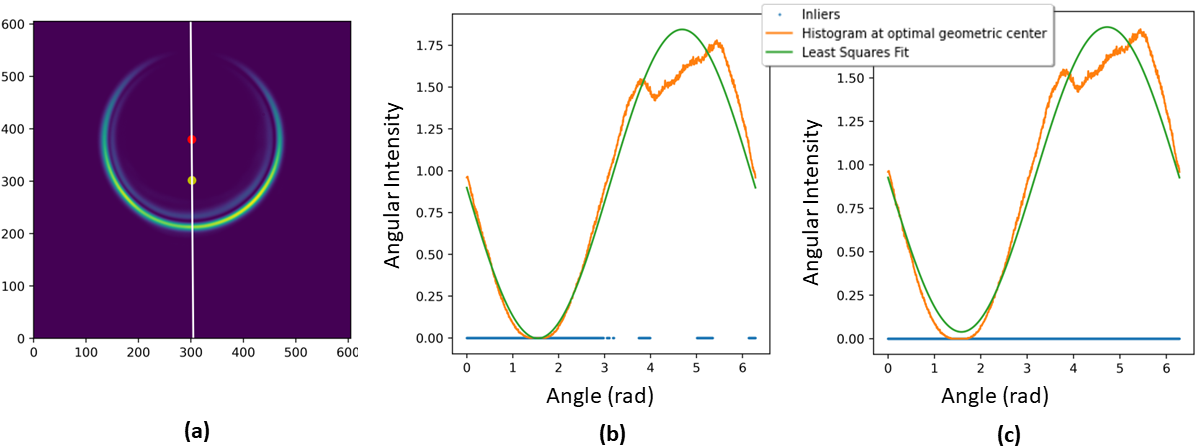
\includegraphics[width=0.8\linewidth]{histo.PNG}
    \caption{ (a) In red, the geometric center found with the Blazquez algorithm. In yellow the gravicenter. The white line indicates the estimated main axis. Using the intensity angular profile of this noisy image around the geometrical center: (a) RANSAC fit of a cosine squared. (c) Least squares fit. Note that in (c), the noisy crests slightly displace the optimal cosine that could be drawn by visual inspection. In (b), we allow to fit the cosine only using the support points in blue (inliers). These were found by RANSAC, which effectively marks the distorted crest as outlier samples.}
    \label{fig:ransac}
\end{figure}

\mybox{{\bf RANSAC\vspace{0.1cm}\\}
In general, the procedure for RANSAC \cite{RANSAC} is the following one:\vspace{-0.2cm}
\begin{enumerate}
\item Given the model to fit (in our case the cosine least square model) and given the noisy observed values $\{(\theta_k,\ \mathcal{I}_k)\}_{k=1}^{N_\theta}$, do the following for a given number of trials.\vspace{-0.1cm}

\item Select a random subset of samples from $\{(\theta_k,\ \mathcal{I}_k)\}_{k=1}^{N_\theta}$ (with a minimum subset size fixed by the user) and fit the model to them.\vspace{-0.1cm}
\item Predict the intensity values given by this fitted model for all the support nodes $\{\theta_k\}_{k=1}^{N_\theta}$ and compute their error with the observed $\{\mathcal{I}_k\}_{k=1}^{N_\theta}$. Define as inliers those points for which the fitted model has an error smaller than a user defined threshold.\vspace{-0.1cm}

\item If the number of inliers is bigger than a certain user-defined tolerance, then estimate again the model, now with all the found inliers and return it.\vspace{-0.1cm}

\item If the maximum iterations are achieved, then return the model of the subset that had the least number of outliers.
\end{enumerate}
}%\vspace{-0.2cm}


\begin{algorithm}
\caption{ \rule{0pt}{3.5mm}{} {\bf The Blazquez + RANSAC Cosine Fit Algorithm } - Pseudo-code\newline To get $\Delta \Phi_{LP}$ use $I\in\{I_{pb},I_{ref}\}$, to get $\Phi_{LP_{pb}}$, $\Phi_{LP_{ref}}$ then $\Delta\Phi_{LP}=\Phi_{LP_{pb}}-\Phi_{LP_{ref}}$.}\label{alg:Mix}
\func{$C(\cdot,\cdot;\ w_{Blz},\ w_{csf},\ s):$\DontPrintSemicolon{\Comment*[r]{\small $C_{Blz}$ def. in alg. \ref{alg:Blaz}, $C_{csf}$ in alg. \ref{alg:cosFit}}}\vspace{-0.4cm}}{
{\bf return } $s\cdot C_{Blz}(\cdot,\cdot;\ w_{Blz})+(1-s)\cdot C_{csf}(\cdot,\cdot;\ w_{csf})$ 
}
\Given{$I,\ \vec{g}_{grav},\ s,\ similarity(\cdot,\cdot)\ N_\theta,\ N_r, \theta_{min}=-\pi, \ \theta_{max}=\pi\ :$}{
$\vec{\theta}s\gets $ equispaced grid of $N_\theta$ points in $(\theta_{min},\theta_{max})$\;
$w_{Blz}\gets\{\ I,\ similarity(\cdot,\ \cdot)\ \} $\;
$w_{scf}\gets\{\ I,\ \vec{\theta}s,\ N_\theta,\ N_r,\ True\ \}$\;
$\vec{g}_{geom}\gets$ 2D min. Search $(\ C(\cdot,\cdot,w_{Blz},w_{scf},\ s) ,\ (c_{x\; min},c_{x\; max})=(0,\; width(I)),\ (c_{y\; min},c_{y\; max})=(0,\; height(I))\ )$\; 
$H\gets$ matrix with $N_\theta$ rows, where k-th row is $[\ 1,\ cos(\vec{\theta}s[k]),\ sin(\vec{\theta}s[k])\ ]$\;
$\vec{x}_{opt} \gets $ RANSAC solve $\vec{x}$ for linear model $\pmb{H}\vec{x}\sim\vec{\mathcal{I}}$ (min\_samples, max\_trials, resid\_thresh)\;
$\Phi_{LP}\gets$ tan$^{-1}(\vec{x}_{opt}[2]/\vec{x}_{opt}[1])$\;
{\bf return } (take to $(-\pi,\pi)$ with alg. \ref{alg:topipi} $\{2\Phi_{LP}\}$)/2\DontPrintSemicolon{\Comment*[r]{It returns $\Phi_{PL}$}}\vspace{0.1cm}}
\end{algorithm}



\newpage
\section*{B.7. Basic Black-Box Algorithms}\vspace{-0.1cm}
\addcontentsline{toc}{subsection}{7. Basic Black-Box Algorithms}
\fancyhead[OR]{ Basic Black-Box Algorithms}
\fancyhead[EL]{ Basic Black-Box Algorithms}
An obvious solution to the problem is to train a neural network (NN) to which we input the crescent ring image and we ask it to output the $\phi_{CR}$ (or the $\Phi_{LP}$) angle. To train it we have practically an infinite number of simulated noisy and non-noisy images of a wide range of possible $R_0,w_0,z,\phi_{CR}$. %\vspace{-0.05cm}

The most basic idea would be to use a fully connected NN \cite{NN} that takes as input the flattened $605\cross 605$ iX standardized images and outputs $\phi_{CR}$. Because the input vector has $605^2=366025$ dimensions, such a NN would need to have many weights to be functional. An option to do this feasible would be to downsample the images before inputting them to the NN. However, we knew the geometrical algorithms (B.6) heavily depended on the resolution of the input images, in a way that the higher their resolution, the predicted results got significantly better. With a similar rationale, on behalf of quantitativeness, we decided not to try this path (it could still be a good option).%\vspace{-0.05cm}

Instead, what seemed more reasonable was to let the neural network learn the required down-sampling. This can be done by fitting successive convolutional layers each of which reduce the size of the input data using trainable weights \cite{NN}. Only after the size of the data is sufficiently reduced a fully connected NN is plugged in. We implemented two variants. We called one of them Encoder A: it reduces the data until very few dimensions before the fully connected. The second one of them, Encoder B, reduces the data only until an intermediate dimension. Then, a larger fully connected network is plugged in. The architecture of each of the two considered encoders is detailed in Table \ref{tab:nns}. The networks were programmed and trained employing Python's {\em PyTorch} library \cite{pytorch}, with an Adam optimization algorithm \cite{adam} and a decaying learning rate. The input images were $iX$ standardized and divided by their maximum value, to take them to a range $[0,1]$.%\vspace{-0.05cm}

More elaborated and deeper NNs than the suggested ones would possibly give quantitatively better results. However, due to the computational resource limitation, by which a single personal use GPU was available, these were not contemplated as a feasible possibility. In addition, the objective device is to be low-cost, which means the cost of a GPU should only be taken if strictly required.%\vspace{-0.05cm}

\begin{table}[h!]
\caption{Architecture of the employed neural networks. From top to bottom, the ordered sequence of applied functions with the shape of their outputs. The networks were trained to be used with our camera's $iX$ standardized images of $X=302$. Thus, the input array in each batch has a shape $[N_{batch}, 1, 605, 605]$, with $N_{batch}$ the number of images in the batch. LR stands for the Leaky Relu activation function, Enc. means Encoder and Tripl. represents the network trained with the Triplet Loss. "Y" means that the network does have the layer of that row, while "N"  means it does not. All the convolutional layers have a stride 1 and 0 padding. The kernel size and the number of filters are then uniquely determined by their output's shape. \vspace{-0.4cm}}\label{tab:nns}
\center
\begin{tabular}{llccc}
\toprule
                              {\bf Layer} &                 {\bf Output Shape} & {\bf Enc. A} & {\bf Enc. B} & {\bf Tripl.} \\
\midrule
                              Input &   $[N_{batch}, 1, 605, 605]$ &         Y &         Y &                Y \\
                     Convolution+LR &  $[N_{batch}, 20, 303, 303]$ &         Y &         Y &                Y \\
       Dropout p=0.2+Convolution+LR &  $[N_{batch}, 20, 182, 182]$ &         Y &         Y &                Y \\
           Batch Norm+Dropout p=0.1 &  $[N_{batch}, 20, 182, 182]$ &         Y &         Y &                Y \\
                     convolution+LR &    $[N_{batch}, 20, 74, 74]$ &         Y &         Y &                Y \\
      Average Pooling+Dropout p=0.1 &    $[N_{batch}, 20, 38, 38]$ &         Y &         Y &                Y \\
           Convolution+Batch Norm.  &       $[N_{batch}, 5, 9, 9]$ &         Y &         Y &                Y \\
                 Average Pooling+LR &       $[N_{batch}, 5, 2, 2]$ &         Y &         Y &                Y \\
               Fully Connected + LR &            $[N_{batch}, 10]$ &         Y &         Y &                Y \\
                   Fully Connected  &             $[N_{batch}, 1]$ &         Y &         N &                N \\
                   Fully Connected  &            $[N_{batch}, 10]$ &         N &         N &                Y \\
 Fully Connected + LR+Dropout p=0.2 &            $[N_{batch}, 10]$ &         N &         Y &                N \\
               Fully Connected + LR &            $[N_{batch}, 10]$ &         N &         Y &                N \\
 Fully Connected + LR+Dropout p=0.1 &            $[N_{batch}, 10]$ &         N &         Y &                N \\
 Fully Connected + LR+Dropout p=0.1 &            $[N_{batch}, 10]$ &         N &         Y &                N \\
                    Fully Connected &             $[N_{batch}, 1]$ &         N &         Y &                N \\
\bottomrule
\end{tabular}
\end{table}
\newpage


\section*{B.8. Embedding Space Algorithms}\vspace{-0.2cm}
\addcontentsline{toc}{subsection}{8. Embedding Space Algorithms}
\fancyhead[OR]{ Embedding Space Algorithms}
\fancyhead[EL]{ Embedding Space Algorithms}

Let us think of the flattened, $iX$ standardized $[2X+1,\ 2X+1]$ images as vectors $\vec{v}$ in a $(2X+1)^2$ dimensional real vector-space. Each of the images is then a point in this $\R^{(2X+1)^2}$ space. Because when we simulate the crescent ring images we determine them only varying four parameters $R_0,w_0,z,\phi_{CR}$, and because all of them cause a continuous change in the image vectors $\vec{v}$ (we forget for a moment they have a limited bit-depth), this suggests that the set of possible crescent ring images forms a 4 dimensional manifold in $\R^{(2X+1)^2}$. We can uniquely label each possible image-vector using four parameters $R_0,w_0,z,\phi_{CR}$ that if continuously varied cause a continuous variation of the corresponding image-vector $\vec{v}$. Thus, we are implicitly defining $\vec{v}(R_0,w_0,z,\phi_{CR})$, a parameterization of the hyper-volume in which the possible CR image-vectors lay, employing just four degrees of freedom. This means there should be a transformation $\vec{\psi}:\R^{(2X+1)^2}\rightarrow\R^4$ that takes the points in $\R^{(2X+1)^2}$ and embeds them in $\R^4$ in a way that every different image-vector $\vec{v}$ goes to a different $\R^4$ point. If the transformation function $\vec{\psi}$ is fast enough, then, this could be a useful representation space for the images, since a classification or regression task could be simpler in a smaller dimensional space. Moreover, we could design the embedder $\vec{\psi}$ to place the samples in a configuration that is more convenient for the labeling of non-labeled samples that we embed between already labeled samples.\vspace{-0.3cm}


\subsection*{B.8.1. Identifying the Dimensionality of the Data Manifold}\vspace{-0.1cm}
%\addcontentsline{toc}{subsubsection}{8.1. Identifying the Dimensionality of the Data Manifold}

Assuming all data lays in such a four dimensional manifold is a bit restrictive and unrealistic. This is mainly because experimental images will always have noise. For each of the possible degrees of freedom in which each noise source can be parameterized, we will be introducing a possibly new degree of freedom in the data manifold (most noise sources generate images that were not among the theoretically perfect $R_0,w_0,z,\phi_{CR}$ crescent rings, so a new curvilinear direction in $\R^{(2X+1)^2}$ will be explored). For example, if we considered the artificial noise we described in (B.2) to be a faithful representation of noise (which is clearly not), then, the number of Gaussian blobs in each image, their location and standard deviations, their strength etc. would also implicitly be involved in the parametric definition of $\vec{v}$. This could lead us to conclude that because there could be an unlimited number of noise factors, experimental data is not in a low dimensional manifold anymore. And that might be true, but even still, it might be useful to choose a low dimensional embedding space representation, because (a), it could be enough for the quantitativeness we seek, or more importantly (b), it could be forced to take the noisy images and send them to the same low dimensional neighborhood, implicitly acting as a de-noiser. That is, a lower dimensional representation could end up "correcting" the data manifold that started to "slip through our fingers" when we began to introduce noise degrees of freedom, and could mould it back to the (ideally 4) lower dimensional manifold. Whether this is possible or not would be determined by whether it is technically possible to tell which is the original "ground-truth" that formed a given noisy image. That is, whether each noisy image can really be uniquely traced back to its Platonic crescent ring: whether the stochastic noise function is injective in a sense. This seems to be an unfair assumption, but could work for many noise sources. Thus, possibly there is a reasonable lower dimensional embedding space where we can fit the data, but this will need to have more than 4 dimensions to allow the accommodation of these "degeneracies".


The question is then: which one is a "reasonable dimension"? For this, we could design embedding functions $\vec{\psi}$ for several dimensions and evaluate how well they preserve the structure of the original dataset. This is what is called in general a "reconstruction error" \cite{manifold}, and we will call the {\em preservation error}. As we keep lowering the dimensionality of the embedding space, the preservation error will clearly keep increasing (for there will be subtle degrees of freedom that will inevitably be lost). Yet, a serious steep increase is expected to appear when we drop the dimension below a certain threhsold, in which many far away samples start to be sent to colliding embeddings. We could geometrically imagine this point as the dimension in which the data manifold no longer "comfortably fits in". Then, this will indicate the effective dimensionality of the data manifold.

To perform this test, we have chosen algorithms that look for embedding functions $\vec{\psi}$ trying to preserve several aspects of the structure of the manifold. These are: the Multidimensional Scaling (MDS) \cite{MDS}, which tries to preserve inter-point distances, the Uniform Manifold Approximation and Projection (UMAP) \cite{umap}, which tries to preserve the topological structure of the manifold, and the NCA algorithm \cite{NCA}, trying to preserve the ability to predict the label of a sample by its proximity to the adjacent points (in a sense trying to preserve the continuity caused by having an equal label). The inner workings of these algorithms are described in (B.8.3).



We can see in Figure \ref{fig:dimension}, the preservation errors found by the MDS, UMAP and NCA methods as a function of the embedding space dimension of the obtained embedders (employing 2000 samples from the noisy image dataset to train them). As reconstruction error for MDS, the stress function characterizing it was chosen, while for NCA and UMAP, a $k=5$ nearest neighbour regression score was employed for a test set of $500$ labeled samples transformed by the trained embedders. We can see that the optimal effective dimensionality of the embedding space could be fixed, in accordance with the three methods, around 10 dimensions. From here on, this dimensionality will be assumed for all the embedding space algorithms of the work.

\begin{figure}[h!] 
     \centering 
    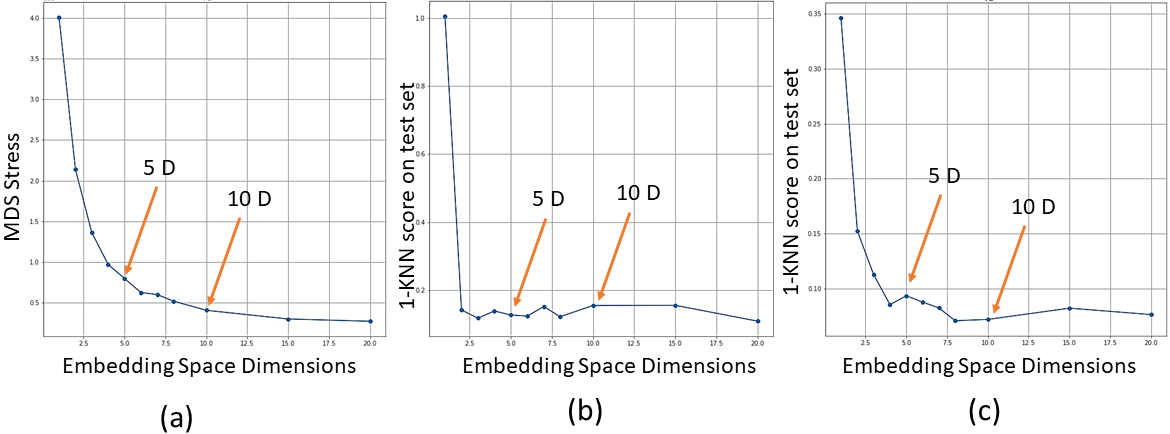
\includegraphics[width=0.9\linewidth]{dim.PNG}
    \caption{(a) MDS stress as a function of the embedding space dimension. (b)  1-KNN Regression score $(k=5)$ by UMAP embedder as a function of embedding space dimension. (c)  1-KNN Regression score $(k=5)$ by NCA embedder as a function of embedding space dimension. }
        \label{fig:dimension}
\end{figure}

\vspace{-0.25cm}

\subsection*{B.8.2. Metric Learning and Nearest Neighbors}
%\addcontentsline{toc}{subsubsection}{8.2. Metric Learning and Nearest Neighbors}

The potential purposes for embedding functions $\vec{\psi}$ in this work are twofold:\vspace{-0.2cm}
\begin{itemize}
\item[(a)] On the one hand, the distance between the images in the embedding space can be used as a similarity metric (to be used in the geometric algorithms (B.6) or the simulation fit algorithms (B.9)). The reason why they could be useful instead of using directly an Euclidean distance metric or the MAE \eqref{MAE} for the un-embedded images, is that some embedding algorithms are trained to evade noise, or to preserve only the most significant variability axes of the data manifold. This can turn out to work as an implicit de-noiser.\vspace{-0.1cm}

\item[(b)] On the other hand, embedding spaces are usually trained to agglomerate data samples with the same or similar labels. Thus, they are the perfect scenario to apply a $K$-Nearest Neighbour (KNN) Regression, which essentially works as follows. Given an unlabeled sample $\vec{v}_{N+1}$, we embed it as $\vec{\psi}(\vec{v}_{N+1})$ and we look for the $K$ closest embedded samples for which we have a label. Then, we predict the label of $\vec{v}_{N+1}$ as the average label of the neighbors, weighted by their distances to the sample. We know that in the original space, the images already varied continuously with the label $\phi_{CR}$, so we could already expect a KNN to work there. If then the embedders are trained to increase the proximity between common labels, the effectiveness of KNN should only increase. In our implementation, we will be using the Ball Tree \cite{balltree} variant of the KNN algorithm to deal with higher dimensional and more numerous datasets, with a $k=3$, as implemented in {\em scikit-learn} \cite{sklearn}. See the procedure followed to get $\Phi_{LP}$ in Algorithm \ref{alg:knn}.
\end{itemize}

 A remaining question is whether we should employ the noisy or the non-noisy dataset to train the embedders and the KNN. For metric learning as well as the KNN, it seems that the noisy dataset should be preferred, for their aim is to include the effect of realistic data (which is noisy). However, for the embedder learning the answer is not that clear. Because noisy data can act as bridges between portions of the manifold that otherwise should not be directly connected, it could happen that the fine local structure of the manifold is spoiled by training them with noisy data. Also, it could happen that if instead we train them with non-noisy data, the embedder acts as a natural denoiser, taking the samples that lay outside the core manifold to "their place". However, it might happen, as we discussed previously, that there are noisy images that could have been generated by different $\phi_{CR}$. A degree of freedom to represent them can only be captured if we use noisy images in the training. Therefore, we will try both approaches and see what is the best one in each case. 
\begin{algorithm}
\caption{\rule{0pt}{3.5mm}{}  {\bf Embedding Space KNN Regression} - High Level Pseudo-Code\newline To get $\Delta \Phi_{LP}$ use $I\in\{I_{pb},I_{ref}\}$, to get $\phi_{CR_{pb}}$, $\phi_{CR_{ref}}$ then $\Delta\Phi_{LP}=(\phi_{CR_{pb}}-\phi_{CR_{ref}})/2$.}\label{alg:knn}
\Given{$I,\ \vec{\psi},\ embedded\_dataset,\ K$ :}{
$I\gets$ $($ iX standardize $(I)\ )/max(I)$\;
$I_e\gets \vec{\psi}(I)$\;
{\small $closest\_labels,\ closest\_dists\gets$ get label ($\phi_{CR}$) and distance to $K$ closest $\vec{\psi}$(samples) in dataset $\null\quad\null\quad\null\quad\null\quad\null\quad\null\quad\null\quad\null\quad\null\quad\null\quad\null\quad\null\quad\null\quad\null\quad\null\quad\null\quad(I_e,\ embedded\_dataset,\ K)$}\;
$\phi_{CR}\gets$  average label weighted by inverse distance $(closest\_labels,\ closest\_dists)$\;
{\bf return } (take to $(-\pi,\pi)$ with alg. \ref{alg:topipi} $\{\phi_{CR}\}$)\DontPrintSemicolon{\Comment*[r]{It returns $\phi_{CR}$}}\vspace{0.1cm}
}
\end{algorithm}\vspace{-0.5cm}


\subsection*{B.8.3. Employed Algorithms to Generate Low Dimensional Embedders}

We offer in what follows a description of each of the employed embedding generation algorithms, together with a visual representation of the embedding spaces generated in each case (for which a PCA is applied on the embedded training samples).

The CNN Triplet Loss embedder was implemented using the {\em Pytorch} library \cite{pytorch} and the custom architecture in Table \ref{tab:nns}. MDS, PCA, KPCA, Isomap and LLE were used through their implementation in the {\em scikit-learn} library in Python \cite{sklearn}. For UMAP, the implementation offered as the {\em umap-learn} \cite{umaplearn} Python library was employed.\vspace{-0.30cm}
\subsubsection*{Triplet Loss Convolutional Neural Network Embedder}\vspace{-0.15cm}
Both to be used as a pre-processing function to run a KNN regression or to be used as a similarity metric, the most ideal of the embedders $\vec{\psi}_{\vec{w}}:\R^{(2X+1)^2}\rightarrow \R^n$ should metrically separate as much as possible semantically different samples (with different $\phi_{CR}$ label) and make as metrically close as possible semantically similar samples (with similar $\phi_{CR}$). We can try to obtain such an embedder by training the parameters $\vec{w}$ of a paramterized emebdding function $\vec{\psi}_{\vec{w}}$, like a NN, with an objective cost function following the stated idea. These kind of cost functions are named as Triplet Losses. Following \cite{triplet}, a feasible implementation to be used in our datasets, where we have almost infinite samples and thus we will perform a batched training, would be to partition the dataset in $PK$ sample batches. $P$ different images $\vec{v}_j^{\phi_{CR_j}}\in\R^{(2X+1)^2}$ of different $\phi_{CR_j}\in(-\pi,\pi]$ are randomly chosen in each batch, and for each of them $K$ random noisy versions $\vec{v}_k^{\phi_{CR_j}}$ with the same label $\phi_{CR_j}$ are sampled. The cost function per each batch is then computed by finding for each sample the hardest possible negative of the batch (which is defined as the sample with different label $\phi_{CR_s}$ that is metrically closest to it) and the hardest possible positive of the batch (the sample with same label $\phi_{CR_j}$ but laying furthest away metrically). Then the cost function $C$ would maximize the first while it minimizes the second one:\vspace{-0.1cm}
\begin{equation}\hspace*{-0.5cm}\small 
C\qty(\vec{w};\ \{\vec{v}_k^{\phi_{CR_j}},\ \phi_{CR_j}\}_{j=1,\ k=1}^{P,\ K})=\sum_{j=1}^P\sum_{k=1}^K\Big[ m+\max_{p=1,...,K}D(\ \vec{\psi}_w(\vec{v}_k^{\phi_{CR_j}}),\ \vec{\psi}_w(\vec{v}_p^{\phi_{CR_j}})\ ) - \min_{\substack{s=1,...,P\\ n=1,...,K\\ s\neq k}}D(\ \vec{\psi}_w(\vec{v}_k^{\phi_{CR_j}}),\ \vec{\psi}_w(\vec{v}_n^{\phi_{CR_s}})\ )\Big]_+\vspace{-0.3cm}
\end{equation}
\newpage
\noindent where $[m+\cdot]_+:=max(m+\cdot,\ 0)$ is called hinge and $m\geq 0$ is called the margin. $D(\cdot,\cdot)$ is a distance function which will be the Euclidean distance in our case. The margin acts as a boundary to stop taking into account samples that are already satisfactorily separated. By this we mean the cases in which the hardest negative of the batch (closest different label sample) is already at least $m$ distance units away from the hardest positive (the farthest same label sample).\vspace{-0.05cm}

In our case we do not mind if this distance gets aribitrarily large, and since we have continuous labels that cause a continuous transition of the images, we will possibly not achieve it anyway. As such, we substitute, following \cite{triplet}, the function $[m+\cdot]_+$ by a smooth approximation using the so called soft-plus function $ln(1+exp(\cdot))$, which is numerically stably implemented in the {\em Pytorch} library \cite{pytorch}. This soft-plus function acts as the hinge but with an exponential decay instead of an abrupt threshold.\vspace{-0.05cm}

With all this in mind, we designed the encoder architecture detailed in Table \ref{tab:nns}, which is an adaptation of Encoder A of section (B.7). It was convenient to start the training already with some significant weights (transfer-learning). Remind from (B.3) that for this training a particular dataset was generated in which chunks of $K$ images of the same label $\phi_{CR}$ are jointly gathered. Each of these chunks contains the non-noisy version of the images. We chose $K=4,P=20$. The training was done in {\em Pytorch} with an Adam optimizer \cite{adam}.\vspace{-0.05cm}

It is interesting to see in Figure \ref{fig:triplet} that as the training progressed (the loss diminishes), the overall norm of the embedding space samples $\vec{\psi}_w(\vec{v}_k)$ increased, accounting for the enlargement of the space. The same happens for the average distance between the embedded samples. As the training progresses, as we expected, the samples get each time farther away from each other. This happens without bounds because of the soft-plus hinge that does not impose a hard margin.\vspace{-0.05cm}

\begin{figure}[h!] 
     \centering 
    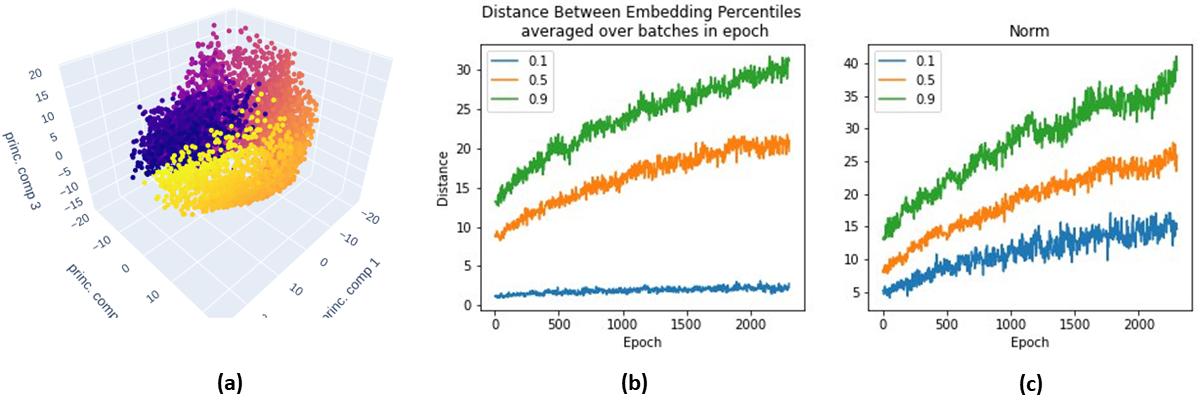
\includegraphics[width=0.8\linewidth]{triplet.PNG}
    \caption{ (a) The Embedded samples using the trained Triplet Loss embedder, reduced dimensionally to 3D using PCA for visualization. (b) Percentiles (see inset) for the distances between embedded samples of the same batches, per epoch (averaged over batches). (c) Percentiles for their norms. }
    \label{fig:triplet}
\end{figure}\vspace{-0.4cm}

\subsubsection*{(Metric) Multi-dimensional Scaling (MDS)}\vspace{-0.1cm}
Given a fixed embedding space dimension $n$ and a representative sub-set of the observable samples $\{\vec{v}_k\}_{k=1}^{N}$ with $\vec{v}_k\in\R^{(2X+1)^2}$ (flattened crescent ring images of varying $R_0,w_0,z,\phi_{CR}$), MDS \cite{MDS} looks for a set of corresponding positions $\{ \vec{e}_k \}_{k=1}^N$ with $\vec{e}_k\in\R^n$, $n<(2X+1)^2$, such that the distances between the samples in the original space $d(\vec{v}_j,\ \vec{v}_k)$ are equal to the distances between the corresponding points in $\R^n$, $d(\vec{e}_j,\ \vec{e}_k)$; with $d(\cdot,\cdot)$ a fixed distance metric.
\mybox{ In our case $d$ will be the Euclidean distance $d(\vec{x}_j,\ \vec{x}_k)=|\vec{x}_j-\vec{x}_k|$, with $|\vec{x}|=\sqrt{\sum_{j=1}^s x_j^2}$ for $\vec{x}=(x_1,...,x_s)\in\R^s$, $s\in\N$. Such a disposition of points, still preserving all their inter-distances in lower dimensions, will typically not be strictly possible; especially if the data manifold dimensionality is greater than the embedding space. Thus, what is typically done is to define a "stress" cost function for a certain point orchestration $\{ \vec{e}_k \}_{k=1}^N$, measuring how close the ensemble is from its ideal inter-disposition. Then, the disposition minimizing this cost is found. A typical stress cost is the root mean square error between the distances in each space:}
\mybox{
\begin{equation}\small
stress\qty(\ \{\vec{v}_k\}_{k=1}^N,\ \{\vec{e}_k\}_{k=1}^n\ )=\frac{1}{N}\sqrt{\sum_{k=1\\ k\neq j}^N\sum_{j=1}^N\qty(\ d(\vec{v}_j,\ \vec{v}_k)-d(\vec{e}_j,\ \vec{e}_k)\ )^2}\vspace{-0.2cm}
\end{equation}
%We employed the implementation in the {\em sklearn} Python library, which implements it using a Scaling by MAjorizing a COmplicated Function (SMACOF) algorithm. It sets an initial starting configuration (in principle randomly), computes its stress, then using it the Guttman transform, and re-iterates till convergence.

Note that unless we employ interpolation, this method does not allow us to embed new samples $\vec{v}_{N+1}$, that are out of the training set $\{\vec{v}_k\}_{k=1}^N$.% Thus it will not be useful for the regression tasks, not either recommended, since if what we relay on for the regression is on the inter-point distances, then better use the exact distances of the training set. However, it is a strong tool to look for the dimensionality of the space in which the training set of samples can be "comfortably" placed (determine the dimensionality of the underlying data manifold from which we sampled them).
}
\vspace{-0.5cm}
\subsubsection*{Uniform Manifold Approximation and Projection (UMAP)}\vspace{-0.15cm}
This is a manifold learning method that unlike many others, has a heavy mathematical machinery backing its consistency, as the original references show \cite{umap,umaplearn}. Qualitatively, the main thing this machinery proves is that the manifold from which the observed set of points $\{\vec{v}\}_{k=1}^N$ is sampled, can faithfully be represented with a simplicial complex (an ensemble of simplices connected with each other through their faces) which at the same time, thanks to the Vietoris-Rips construction, can reasonably be described by only using 0- and 1-simplices (points and lines) $-$ generating a graph. The main result backing this correspondence comes from the so called "Nerve theorem" \cite{ umap}, by which the simplicial complex is homotopicaly equivalent to the manifold. Then, the key idea is that if the same complex is replicated in a lower dimensional space, we can have certainty that the complex represents a topologically equivalent manifold in lower dimensions. 

\mybox{The question is then: how can we create such a simplicial complex? If we had an open cover of the manifold, like a set of balls whose union covers the whole manifold, this can be done by making correspond the centers of the balls with 0-simplices or vertices, while each intersection between the open sets is made to correspond with a 1-simplex or edge, connecting the vertices of their centers; higher dimensional simplices could then be considered for multi-set intersections (this would account for the Čech construction). Yet, we only know that the observed points $\{\vec{v}_k\}_{k=1}^N$ lay in the manifold. The big merit of the UMAP algorithm \cite{umap} is to provide a way to construct the simplicial complex using only the sampled points $\vec{v}_k$ instead of a proper open cover of the manifold. For this, the sampled points $\vec{v}_k$ (which are sure part of the manifold) are used as centers of balls that will approximate a probabilistic open cover of the data manifold (where the bigger the ball the less likely it will be considered to be included in the manifold). With this, a so called "fuzzy simplicial complex" is built following a similar procedure as the commented one. This way, the observed points (which are the centers of the balls) will correspond with the vertices of the graph. The difference will be that now, the bigger the radious of the balls when the intersections occur, a smaller weight will be set to the edge connecting its centers. We can interpret these weight on the edges as the probability for that edge to pertain to the complex and thus to be a descriptor of the underlying manifold. Then, once this weighted graph in $\R^{(2X+1)^2}$ is built, we will seek to get a set of observed point embeddings in a lower $n$ dimensional space $\{\vec{\psi}(\vec{v}_k)\}_{k=1}^N$, such that the fuzzy complex they represent is as similar to the bigger dimension one as possible. This can be done by minimizing the binary cross entropy relating the weights of the two graphs.\vspace{0.2cm}

One of the most important points the underlying mathematical machinery solves here is that in reality what we have stated should only be true if the sampled points $\vec{v}_k$ were homogeneously distributed in the manifold. If this is not true (as is the case typically), the generated balls of fixed radii can fail to cover the whole manifold and it could happen that under-sampled regions appear to be isolated islands (when the number of connected components is a property preserved by homotopy). To solve this, UMAP considers a metric by which the points are indeed uniformly distributed. This trick is done with a locally varying metric (a Riemannian metric), such that the radious of the ball is weighted by the distance to the $K$-th nearest neighbour (in Euclidean terms), for a fixed $K$. In particular, the unit ball around each point is made to stretch until the $K$-th nearest neighbor. This way, the points that were in under-represented regions of the manifold can be more fairly connected to the rest of nearby points. Not to favor the preservation}\mybox{ of their distance, but the local connectivity of the manifold. Then, since the probability weights of the edges were computed as a function of the radial distance to the overlap spot, this allows the under-sampled regions to be locally connected to the surrounding manifold. In fact, to avoid vertices that are even still left isolated, in order to consider the localities of the manifold connected, every point is considered to be connected (with probaility 1) at least to its nearest neighbour. It is at this radious and not before when the decay of probability as a function of the "Riemanian radious" is considered.\vspace{0.2cm} % As a function of the $K$ chosen here, the description of the manifold will have a varying degree of local detail. If $K$ is very big, the local metric structure of the immediate neighbourhood of each point will be lost. Yet, if $K$ is too small, we will loose the global structure of the manifold.\\ %It is worth noting that this method then produces edges from a point to another that can have two different weigths (as a function of the local metric considered for the origin vertex). This is solved by considering them both probaiblistic edges, that are unified as the probability that at least one of them is a true edge in the complex. Also, it must be said that to avoid vertices that are left isolated even still, meaning the localities of the manifold are modeled as connected (while globaly there could be several connected componenets), every point is considered to be connected (with probaility 1) at least to its nearest neighbour. Thus it is at this radious and not before when the decay of probability as a function of the "Riemanian radious" is considered. This way we also consider the distances between the neighbours as oposed to the absolute distances. }

Because the low dimensional representation will be built {\em ad hoc}, a distance metric that does not vary in space, like the Euclidean one, can be chosen to construct the graph of the embedded set of points. In consequence, a fixed constant distance to the nearest neighbour $d_{NN}$ is a required parameter, and the resulting embedded training points will seem to be uniformly distributed.
}\vspace{-0.45cm}

\subsubsection*{Neighborhood Component Analysis (NCA)}\vspace{-0.2cm}
The essential idea of Neighborhood Component Analysis \cite{NCA} is to find a linear application $\pmb{A}$ (represented by an $n\cross (2X+1)^2$ matrix) taking the image-vectors in $\R^{(2X+1)^2}$ to $\R^n$, in a way that the closest points in the embedding space have common labels. 

\mybox{To do so, a (normalized) probability function is defined for each $k$-th sample $\vec{v}_k$ in $\{\vec{v}_k\}_{k=1}^N$, with the other samples $j\in\{1,...,N\}\setminus\{k\}$ as support, employing a soft-max function, where the closer the $j$-th sample in the embedding space gets to it, the higher the probability will be:
\begin{equation}\small
P(j|k)=\frac{e^{-|\pmb{A}\vec{x}_k-\pmb{A}\vec{x}_j|^2} }{\sum_{s\neq k}e^{-|\pmb{A}\vec{x}_k-\pmb{A}\vec{x}_s|^2} }
\end{equation}
If we were to take a random neighbour around the $k$-th sample weighted by how close it is, $P(j|k)$ would represent the probability with which we would take the $j$-th sample. Then, denote the points with the same label (or close enough label for a defined number of decimal places) as the $k$-th sample by $S_k$. $P_k:=\sum_{j\in S_k}P(j|k)$ would be the probability that we classify sample $k$ correctly in a $k=1$ KNN. What NCA does then is to take the sum of all these probabilities, which only depend on $\pmb{A}$ (and the sample set), $f(\pmb{A}):=\sum_kP_k$, and looks for the $\pmb{A}$ that maximizes it. $f$ turns out to be differentiable, so efficient optimization techniques can be used.
}
\vspace{-0.45cm}

\subsubsection*{Principal Component Analysis (PCA)\vspace{-0.2cm}}
This is a well known classical method  \cite{PCA}. Essentially it takes the input data (without the need for labels) $\{\vec{v}_k\}_{k=1}^N$, organizes it in a $[(2X+1)^2,\ N]$ matrix $\pmb{X}$ with the data vectors as columns and runs a singular value decomposition $\pmb{X}=\pmb{U}\pmb{\Sigma}\pmb{V}^t$ (with $\pmb{\Sigma}$ the ordered diagonal singular value matrix). The left-singular vectors with highest singular values (columns of $\pmb{U}$) geometrically represent the directions in feature space along which the samples have maximum variation. These directions are particular linear combinations of the features, which in our case are the input image pixels. Then, by assuming that what gives discriminative power is having a bigger variability in the describing features of a sample, we just leave the $n$ most informative ones, corresponding to the biggest magnitude singular values. The space spanned by their left singular vectors would be the embedding space. 
\mybox{
It is easy to see that these left singular vectors are also the $n$ eigenvectors with highest eigenvalues of the covariance matrix of the data, computed as $\pmb{X}\pmb{X}^t$. In particular that: $\pmb{X}\pmb{X}^t=\pmb{U}\pmb{\Sigma}^2\pmb{U}^t$.\footnote{It is also easy to see that for $\pmb{X}^t\pmb{X}$, the dot product matrix, $\pmb{X}^t\pmb{X}=\pmb{V}\pmb{\Sigma}\pmb{V}^t$ is a diagonal decomposition.} This confirms that these $n$ directions are the ones with maximum statistical variance (the eigenvalues of the covariance matrix are the variances, which are the square of the singular values of $X$).%\vspace{0.13cm}
}
\mybox{
The embedding space transformation $\vec{\psi}$ is then given by the change of basis to the left-singular vector basis erasing all but the $n$ most significant coefficients: given $\vec{v}$ this is just a linear application $\vec{\psi}(\vec{v}\,)=\pmb{U}_{n}^t\vec{v}$ (where $\pmb{U}_{n}$ is given by leaving the first $n$ columns of $\pmb{U}$). \vspace{-0.13cm}
}\vspace{-0.15cm}

It is a non-supervised dimensionality reduction method. That is, it does not employ the label information to generate the embedder. Thus, it possibly destroys part of the information that was relevant for label prediction. Yet, it is true that the chosen singular axes could turn out to represent the $R_0,w_0,z,\phi_{CR}$ degrees of freedom, for they are for sure implicated in the biggest of the variations in the resulting image intensity values (more than most noise sources). Thus, it could happen that the information "it destroys" is precisely the jitter introduced by noise.

\begin{figure}[h!] 
     \centering 
    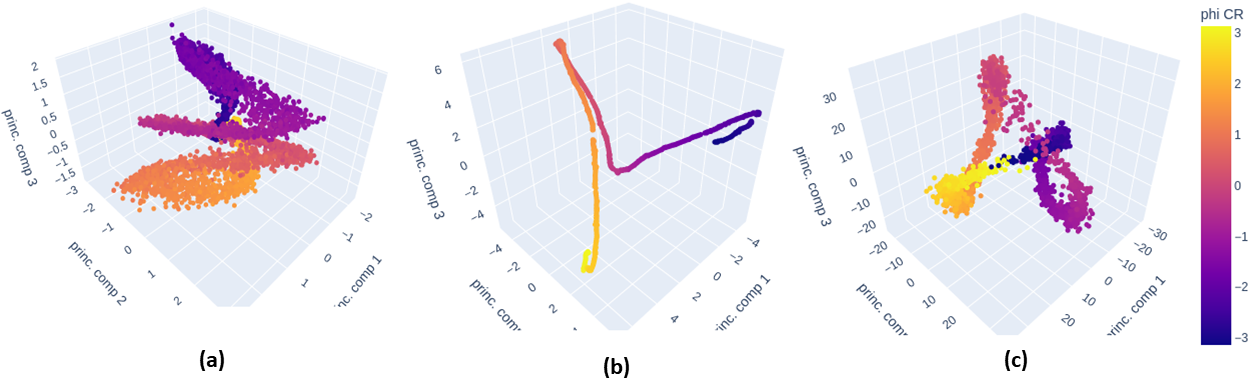
\includegraphics[width=0.95\linewidth]{emb1.PNG}
    \caption{ Samples of the noisy dataset embedded using the trained embedders to 10D, and reduced dimensionally using PCA to 3D for visualization. (a) PCA, (b) UMAP, (c) NCA.  }
    \label{fig:embeddings1}
\end{figure}

\vspace{-0.55cm}

\subsubsection*{Kernel PCA}\vspace{-0.2cm}
Kernel PCA \cite{KPCA}, implicitly embeds first the data into a higher dimensionality space than the data feature dimensions $(2X+1)^2$, to then take its first $n<(2X+1)^2$ principal components (using PCA). The rationale of doing this is that even if in the original feature space differently labeled samples could not be separated by means of simple boundaries (like hyperplanes), if we throw them into a higher dimension, we could arrange them to be easily separable. Then, by only taking the $n$ most informative directions of this high dimensional space we may still be able to separate the labels easily, now in a lower dimension.

\mybox{Given the embedder function to high dimensions is denoted by $\vec{\Lambda}$, this can be done avoiding the computation of the high dimensional embeddings $\vec{\Lambda}(\vec{v}_k)$ explicitly. Our goal is the singular value decomposition of $\Lambda(\pmb{X})$ (which is to apply $\vec{\Lambda}$ to each column of $\pmb{X}$). Following the previous notation, $\Lambda(\pmb{X})=\pmb{U}\pmb{\Sigma}\pmb{V}^t$. The only thing we need is an expression for the dot product of the embeddings $Q(\vec{v}_k, \vec{v}_j)=\vec{\Lambda}(\vec{v}_k)^t\vec{\Lambda}(\vec{v}_j)$ (known as a kernel). With it, the tractable [N,N] dot product matrix $\Lambda(\pmb{X})^t\Lambda(\pmb{X})$ can be computed, as $Q(\Lambda(\pmb{X}), \Lambda(\pmb{X}))$. We saw that computing its diagonal decomposition we get $\Lambda(\pmb{X})^t\Lambda(\pmb{X})=\pmb{V}\pmb{\Sigma}^2\pmb{V}^t$. Then given a sample $\vec{v}$, notice that $\pmb{U}^t\vec{v}=\Sigma^{-1}\pmb{V}^t\Lambda(X)^t\vec{\Lambda}(\vec{v})=\pmb{\Sigma}^{-1}\pmb{V}^tQ(X,\vec{v})$. This means we can get the $n$ dimensional embedding function by only leaving the highest $n$ singular values and vectors in $\pmb{\Sigma},\pmb{V}$ (to form $\pmb{\Sigma}_n,\pmb{V}_n$) and computing $\vec{\psi}(\vec{v})=\pmb{\Sigma}_n^{-1}\pmb{V}_n^tQ(X,\vec{v})$. For which we avoided the explicit use of $\vec{\Lambda}$ in all the steps. In particular, we will employ a radial basis kernel $Q(\vec{v}_k,\vec{v}_j)=exp(-\gamma |\vec{v}_k-\vec{v}_j|^2)$ for $\gamma\in\R$.
}
\vspace{-0.55cm}

\subsubsection*{Isomap}\vspace{-0.2cm}
This is a version of MDS that allows a better preservation of the manifold's local connectivity \cite{isomap}. 

\mybox{For this, first each sampled point from the underlying manifold $\{\vec{v}_k\}_{k=1}^N$ is connected to its $K$}\mybox{  nearest neighbors, for a fixed $K$, forming a weighted graph. The weights of the edges are computed as the distances (Euclidean ones in our case) between the vertices. Once this neighborhood graph is built, the so called graph-geodesic distance between every pair of points is computed. This is, given the shortest path in the neighborhood graph between them (the geodesic path in the graph), the sum of the weights of the path (the distance along the graph). Note how this distance can be way larger than the actual Euclidean distance. The neighbourhood graph will roughly represent the underlying manifold (following a similar intuition -even if not as grounded- as UMAP), so the geodesic path represents the shortest trajectory between the points restricted to the manifold. The distances through the graph, will then encode the disposition of the manifold. With all, the MDS algorithm is applied to build a lower dimensional graph with the same geodesic distances, which will presumably carry the local structure of the manifold. %The $K$ parameter will control the locality of the approach, just like in UMAP.
}
\vspace{-0.35cm}
\subsubsection*{Locally Linear Embedding (LLE)}\vspace{-0.2cm}
The LLE method \cite{LLE}, just as Isomap, looks to preserve the local structure of the manifold.

\mybox{ Fixing a $K$, for each sampled $j$-th point, the $K$ nearest neighbours $\sigma_j$, are first found. Next, by minimization of the cost function $C_1(w_{ij})=\sum_{j=1}^N \qty[\vec{v}_j-\sum_{k\in\sigma_j}w_{kj}\vec{v}_k]^2$, each point is approximated as well as possible as a linear combination of its $K$ nearest neighbours (where in addition the condition $\sum_{k\in\sigma_j}w_{kj}=1$ is imposed). Then, a lower dimensional embedding is found by minimizing a second function, where now the parameters to optimize are the positions $\{\vec{e}_k\}_{k=1}^N$, $\vec{e}_k\in\R^n$, in the embedding space. This cost is $C_2(\vec{e}_k)=\sum_{j=1}^N \qty[\vec{e}_j-\sum_{k\in\sigma_j}w_{kj}\vec{e}_k]^2$ which means we try to still be able to write the embedded points as the same linear combination of its embedded neighbours.}
 
\begin{figure}[h!] 
     \centering 
    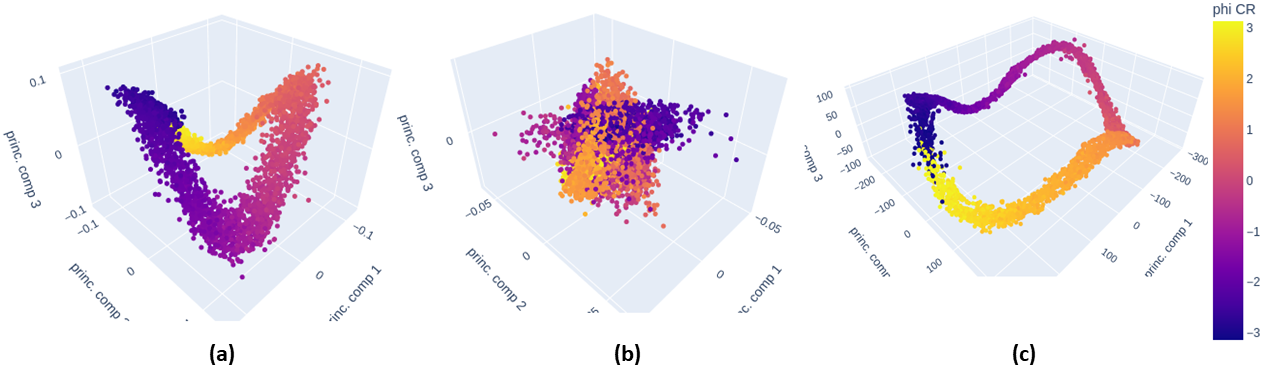
\includegraphics[width=0.96\linewidth]{emb2.PNG}
    \caption{ Samples of the noisy dataset embedded using the trained embedders to 10D, and reduced dimensionally using PCA to 3D for visualization. (a) KPCA, (b) LLE, (c) Isomap.  }
    \label{fig:embeddings2}
\end{figure}

\section*{B.9. Simulation Fitting Algorithms}
\addcontentsline{toc}{subsection}{9. Simulation Fitting Algorithms }
\fancyhead[OR]{ Simulation Fitting Algorithms}
\fancyhead[EL]{ Simulation Fitting Algorithms}
Because we can simulate the crescent rings that should appear in the experimental images if all the theoretical considerations were in order, an obvious algorithm to try is to fit theoretical images to the desired experimental ones until we find a perfect match. That is, not only could we estimate $\phi_{CR}$ and thus $\Phi_{LP}$, but also all the other theoretical degrees of freedom $R_0,w_0,z$. In fact, we could perform a 4D multidimensional optimization to look for the simulated image that is most similar to the experimental one. This algorithm is clearly slower than the rest of the suggested ones, because the simulation of each theoretical image in the optimization takes a considerable time. We can fasten it, by considering the D matrix trick explained in (B.3), yet, it will still not be the fastest one of the algorithms. However, ideally it should be a very precise algorithm for images with low noise, so it is worth giving it a try. 

The similarity metric employed in this search will seriously affect both the optimization landscape and the final result. Fortunately, the Triplet Loss Embedder of the previous section can be employed as a perfect metric for this method: it was trained to make noisy images of the same $\phi_{CR}$ be metrically as close as possible to their non-noisy version. Thus, comparing theoretical images with experimental noisy ones should be carried away with ease by such a metric.

In principle, the equations in (A.3) generate crescent ring images centered in the geometrical centers. For the experimental images on the other hand, in principle we only know their gravicenter. Thus, the immediate algorithm to compare a simulated image with an experimental one would be to first center the simulation as well in its gravicenter (through the iX standard), then, to apply a common pre-processing to take both images to the same intensity ranges. We implemented this method following Algorithm \ref{alg:simul}, by using the Mother Dataset of (B.3) as the simulated image grid.



\begin{algorithm}
\caption{ \rule{0pt}{3.5mm}{} {\bf The Simulation Fit Algorithm (Gravicenter)} - {\small High Level Pseudo-Code}\newline To get $\Delta \Phi_{LP}$ use $I\in\{I_{pb},I_{ref}\}$, to get $\phi_{CR_{pb}}$, $\phi_{CR_{ref}}$ then $\Delta\Phi_{LP}=(\phi_{CR_{pb}}-\phi_{CR_{ref}})/2$.}\label{alg:simul}
\func{$C_{sim}(\  R_0,w_0,z,\phi_{CR};\ I,\  mother\_dataset,\ similarity(\cdot,\cdot),\ pre\_process(\cdot) \ ):$}{
\DontPrintSemicolon{\Comment*[r]{\footnotesize Dataset contains [2,2] D matrices per $[H_{simul},W_{simul}]$ pixel as explained in B.4.}}
{\small $D\gets$ get closest $(R_0,w_0,z)$ D matrix in $mother\_dataset$} \Comment*[r]{\footnotesize Array of shape $[2,2,H_{simul},W_{simul}$]}
{\small $D\_vectors\gets $ matrix dot vector $(D,\ [cos(\phi_{CR}), sin(\phi_{CR})])$} \Comment*[r]{\footnotesize Shape $[2,\ H_{simul},\ W_{simul}]$}
$I_{simul}\gets$ complex Euclidean norm $(D\_vectors)$ \Comment*[r]{\footnotesize Remember $I(x,y)=|\vec{D}(x,y)|^2$}
$I_{simul}\gets $ pre\_process$(I_{simul})$ \;
{\bf return } -similarity $(I_{simul}, I)$\vspace{0.1cm}
}
\Given{\small$I,\ mother\_dataset,\ similarity(\cdot, \cdot),\ pre\_process( \cdot ),$\\ $\null\hspace{2cm}(R_{0min}, R_{0max}),\ (w_{0min},w_{0max}),\ (z_{min},z_{max}),\ (\phi_{CRmin},\ \phi_{CRmax}):$}{
$I\gets $ iX standardize ( pre\_process$(I)$ )\;
$w\gets \{ I,\ mother\_dataset,\  similarity(\cdot , \cdot),\ $iX\_standardize$(pre\_process(\cdot))\}$\;
$R_0,w_0,z,\phi_{CR}\gets$ 4D min. Search $(\  C_{sim}(\cdot,\cdot,\cdot,\cdot;w), (R_{0min}, R_{0max}),\ (w_{0min},w_{0max}),\ (z_{min},z_{max}),\ (\phi_{CRmin},\ \phi_{CRmax})  \ )$\;
{\bf return } (take to $(-\pi,\pi)$ with alg. \ref{alg:topipi} $\{\phi_{CR_1}\}$)\DontPrintSemicolon{\Comment*[r]{It returns $\phi_{CR}$}}\vspace{0.1cm}

}

\end{algorithm}

An alternative version was implemented following Algorithm \ref{alg:simul2}. It uses the fact that the Blazquez algorithm (B.6.7) is very good at finding the geometric center of noisy images, with a precision presumably better than the precision with which we estimate the gravicenter. Then, it is the experimental images that are centered in the geometric centers, before comparing with the simulations, which are centered likewise by default.

\begin{algorithm}
\caption{ \rule{0pt}{3.5mm}{} {\bf The Simulation Fit Algorithm (Geometric Center)} - {\small Pseudo-Code}\newline To get $\Delta \Phi_{LP}$ use $I\in\{I_{pb},I_{ref}\}$, to get $\phi_{CR_{pb}}$, $\phi_{CR_{ref}}$ then $\Delta\Phi_{LP}=(\phi_{CR_{pb}}-\phi_{CR_{ref}})/2$.}\label{alg:simul2}
\Given{\small$I,\ mother\_dataset,\ similarity(\cdot, \cdot),\ pre\_process( \cdot ),\ C_{Blz}$ of alg.\ref{alg:Blaz}$,\ C_{sim}$ of alg.\ref{alg:simul}$,$\\ $\null\hspace{2cm}(R_{0min}, R_{0max}),\ (w_{0min},w_{0max}),\ (z_{min},z_{max}),\ (\phi_{CRmin},\ \phi_{CRmax}) :$}{
$I\gets $ iX standardize ( pre\_process$(I)$ )\;
$w\gets\{\ I,\ similarity(\cdot,\ \cdot)\ \} $\;
$\vec{g}_{geom}\gets$ 2D min. Search $(\ C_{Blz}(\cdot,\cdot;w),\ (c_{x\; min},c_{x\; max})=(0,\; width(I)),\ (c_{y\; min},c_{y\; max})=(0,\; height(I))\ )$\; 
$I_{geom}\gets $ iX standard but using alternative center $(I,\ \vec{g}_{geom})$

$w\gets \{ I_{geom},\ mother\_dataset,\  similarity(\cdot , \cdot),\ pre\_process(\cdot)\}$\;
$R_0,w_0,z,\phi_{CR}\gets$ 4D min. Search $(\  C_{sim}(\cdot,\cdot,\cdot,\cdot;w), (R_{0min}, R_{0max}),\ (w_{0min},w_{0max}),\ (z_{min},z_{max}),\ (\phi_{CRmin},\ \phi_{CRmax})  \ )$\;
{\bf return } (take to $(-\pi,\pi)$ with alg. \ref{alg:topipi} $\{\phi_{CR}\}$)\DontPrintSemicolon{\Comment*[r]{It returns $\phi_{CR}$}}\vspace{0.1cm}

}

\end{algorithm}

\section*{B.10. Pipeline to Compare the Algorithms and Preprocessings}
\addcontentsline{toc}{subsection}{10. Pipeline to Compare The Algorithms and Preprocessings }
\fancyhead[OR]{ Pipeline to Compare the Algorithms}
\fancyhead[EL]{ Pipeline to Compare the Algorithms}
\vspace{-0.3cm}
For each algorithm we have several possible variants, since we have several pre-processing functions, several optimization methods, several embedders etc. In order to estimate the performance of all of them and find the best configurations and best overall algorithms, we run a pipeline of tests employing both the noisy simulated image dataset and non-noisy image dataset, annotating the absolute errors in the prediction of $\Delta\Phi_{LP}$ and the times taken to get these results. The non-noisy dataset will test the precision and timing of the algorithms in the best of the cases, for all the range of acceptable $R_0,w_0,z$ crescent rings, {\bf conditioned on the resolution of the camera being $540\times 540$}. The noisy dataset on the other hand, will test the robustness of the algorithms against very noisy conditions (considerably noisier than the experimentally found ones), for all the range of acceptable $R_0,w_0,z$ crescent rings (the "worst case-scenario"); again assuming the camera resolution is the fixed one.

The pipeline runs the following steps for each of the tested algorithm variants:\vspace{-0.3cm}
\begin{enumerate}
\item A given number of pairs of images from the dataset is inputed in batches to the algorithm (to be used as reference and problem images). The algorithm computes $\Delta \Phi_{LP}$ for each pair and notes the times taken per pair. For the algorithms that process the samples in batches (like the NN algorithms (B.7)), an equal average time for each image is considered.

\item Using the ground truth angle difference $\Delta \Phi_{LP}$, the absolute error is computed for each image pair. This is done taking into account the periodicity of the interval $(-\pi/2,\pi/2]$, meaning that a predicted absolute error $e$ that is bigger than $\pi/2$ is in reality an error $\pi-e$.

\item The sample mean and sample standard deviation for the absolute error and times are computed. Employing them together with the observed values, we build $90\%$ non-parametric bootstrap-t confidence intervals of the population expected error and time for the algorithm.

\item Histograms of the error and time results for the algorithm, with the confidence intervals and the population mean, are plotted.

\end{enumerate}\vspace{-0.3cm}

\mybox{{\bf Non-Parametric Bootstrap-t Confidence Interval \vspace{0.12cm}}\\
Given a set of observations (of time or absolute error in our case) assumed to be generated by a random variable, we can estimate confidence intervals for its population statistics by assuming that the set of observations itself is a representative discretization of the probability distribution. Then, the non-parametric bootstrap-t confidence interval for its statistics is knwon  \cite{boots} to be computable as:\vspace{-0.15cm}
\begin{enumerate}
\item Simulate as many re-samplings form the dataset as possible with reposition (that is, assume it is the discretization of the random variable). For each of them calculate the statistic of interest (we will call it the bootstrap estimate $\hat{\theta}_{boots}$), which in our case is the sample mean.
\item  Assuming you know an expression for the standard error of the statistic, calculate it for each bootstrap sample: $\hat{se}_{boots}$. Then compute the following parameter in each of the resamplings: $t_b=(\hat{\theta}_{boots}-\hat{\theta})/\hat{se}_{boots}$, where $\hat{\theta}$ is the estimation obtained using the truly observed set and $\hat{se}_{boots}$ its standard deviation.
\item  Defining $t_{\alpha/2}$ and $t_{1-\alpha/2}$ as the $\alpha$ outermost quantiles of the accumulated bootstrap $t_b$
parameters, the confidence interval for the desired statistic will be: $(\hat{\theta}+t_{\alpha/2}\hat{se},\ \hat{\theta}+t_{1-\alpha/2}\hat{se})$.
\end{enumerate}
}\vspace{-0.2cm}

\subsection*{B.10.1. Results on the Simulated Datasets}\vspace{-0.2cm}
All the carried tests and their results, gathered algorithm-wise and image-wise can be found in the {\em /RESULTS} folder in the Github repository of the project \cite{github}. In Tables \ref{tab:noisy} and \ref{tab:nonnoisy} we gather only the results of the best found configuration of each algorithm (best combination of pre-processing, embedding function, hyperparameters etc.) for the noisy and non-noisy simulated image datasets respectively. We consider the best variant of an algorithm to be the one providing the lowest upper bound of the confidence interval for the expected absolute error.\vspace{0.2cm} 



\begin{table}[h!]
\caption{Summary of the best variant found for each algorithm on 1000 random samples of the {\bf Non-Noisy} Image Dataset. CI stands for the bootstrap-t confidence intervals for the expectation. Ordered by increasing mean absolute.}\label{tab:nonnoisy}
\hspace{-0.6cm}\begin{tabular}{c|c|c|cc|cc}
\toprule
\multicolumn{2}{c|}{\bf Algorithm} &  \multicolumn{3}{|c|}{\bf Absolute Error (rad)} & \multicolumn{2}{|c}{\bf Times (s)} \\ \midrule \midrule
{\bf                     Name} &                          {\bf Winner} {\bf Variant} &  {\bf Mean} &  \multicolumn{2}{c|}{\bf 90\% CI } &  \multicolumn{2}{|c}{\bf 90\% CI }\\
\bottomrule\rule{0pt}{4mm}{}
           Mirror Flip & Quadratic Opt., Lanczos Interpol.,  & 0.00106 &    0.00102 &   0.00109 &        0.218 &       0.220 \\
                       &               Preproc. Norm. to Max &         &            &           &              &             \\ \hline\rule{0pt}{4mm}{}
Gravicenter Regression &               Preproc. Norm. to Max & 0.00196 &    0.00189 &   0.00203 &        0.453 &       0.454 \\ \hline\rule{0pt}{4mm}{}
  Kalkandjiev-Rotation &  Quadratic Opt., Lanczos Interpol., & 0.00205 &    0.00198 &   0.00213 &        0.221 &       0.222 \\
                       &               Preproc. Norm. to Max &         &            &           &              &             \\ \hline\rule{0pt}{4mm}{}
 Blazquez + Cosine Fit &         w=0.999, Nelder-Mead Opt.,  & 0.00455 &    0.00437 &   0.00475 &        3.38 &       3.39 \\
                       &               Preproc. Norm. to Max &         &            &           &              &             \\ \hline\rule{0pt}{4mm}{}
     Cosine Square Fit &               Preproc. Norm. to Max & 0.00466 &    0.00452 &   0.00480 &        2.820 &       2.830 \\ \hline\rule{0pt}{4mm}{}
              Blazquez &               Preproc. Norm. to Max & 0.124 &    0.0517 &   0.274 &        0.454 &       0.456 \\ \hline\rule{0pt}{4mm}{}
              Simulation Fit	& Opt. Nelder-Mead, About Grav.&	0.140	 & 0.123	& 0.171&	1.283	&1.316\\ 
           &  Preproc. Norm. to Max & & & & \\ \hline
           \rule{0pt}{4mm}{}
          KNN+Embedder &              NCA Embedder, Trained  & 0.280 &    0.140 &   2.32 &        0.130 &       0.160 \\
                       &                 with Non-Noisy Data &         &            &           &              &             \\ \hline\rule{0pt}{4mm}{}
                   KNN &         Trained with Non-Noisy Data & 0.820&    0.484 &   1.40 &        4.960 &       5.610 \\ \hline\rule{0pt}{4mm}{}
     Bimodal Histogram &               Preproc. Norm. to Max & 1.66 &    1.58 &   1.76 &        0.131 &       0.132 \\ \hline\rule{0pt}{4mm}{}
     Relative Rotation & Quadratic Opt., Bicubic Interpol.,  & 1.73 &    1.61 &   1.83 &        0.068 &       0.069 \\
                       &               Preproc. Norm. to Max &         &            &           &              &             \\ \hline\rule{0pt}{4mm}{}
    Polar Registration &               Preproc. Norm. to Max & 2.83 &    2.64 &   3.04 &        0.245 &       0.245 \\ \hline\rule{0pt}{4mm}{}
                CNN+fc &                           Encoder A & 3.41 &    2.94 &   4.06 &        1.093 &       1.094 \\
\bottomrule
\end{tabular}

\end{table}



We find that for the given camera resolution, in the best-case-scenario, the Mirror Flip algorithm is the best algorithm, allowing the determination of the linear polarization angle with a precision of $\pm 0.001$ deg. Note that if we performed the same study with a bigger resolution, the results would be orders of magnitude better, as preliminary checks have shown us. The exact dependence and the asymptotic limit will be studied in a future work. The Mirror Flip algorithm in addition, is capable of determining the angle within a fifth of a second. This speed would be slightly reduced by higher resolution images. Yet, the current implementation in Python is not thought to be the fastest one. Ad hoc optimization, writing the algorithms in a lower level language like C, would make them faster.

On the other hand, the results on the noisy image dataset show that the robustest algorithms in front of noise are the Simulation Fit and the Kalkandjiev-Rotation, closely followed by the Mirror Flip algorithm. The first one offers the smallest mean absolute error of $\pm 1.86$ deg, compared with the $\pm 1.93$ deg of the second one, but taking more time (1.24 s against 0.22 s). This time difference can be very significant, because for real-time measurements it is desirable to have more than one measurement per second.

Some additional points must be noted on the results. On the one hand, we see that the deep learning approaches have performed very poorly: the convolutional encoders are the worst algorithms and the Triplet Loss embedder is neither the best embedder for KNN, nor the best metric for the Simulation Fit. This is possibly due to the limited training of the networks and to the fact that we could not try different hyperparamter and architecture combinations. Also, it could be that networks built from scratch need better losses or way more time of training to achieve quantitative results as the ones we require. Trying a transfer learning from pre-trained networks on more difficult computer vision problems, is something left as future work.
\vspace{0.15cm}

\begin{table}[h!]
\caption{Summary of the best variant found for each algorithm on 1000 random samples of the {\bf Noisy} Image Dataset. CI stands for the bootstrap-t confidence intervals for the expectation. Ordered by increasing mean absolute.}\label{tab:noisy}

\hspace{-0.6cm}\begin{tabular}{c|c|c|cc|cc}
\toprule
 \multicolumn{2}{c|}{\bf Algorithm} &  \multicolumn{3}{|c|}{\bf Absolute Error (rad)} & \multicolumn{2}{|c}{\bf Times (s)} \\ \midrule \midrule
{\bf                     Name} &                          {\bf Winner} {\bf Variant} &  {\bf Mean} &  \multicolumn{2}{c|}{\bf 90\% CI } &  \multicolumn{2}{|c}{\bf 90\% CI }\\
\bottomrule\rule{0pt}{4mm}{}
           Simulation Fit &         Opt. Powell, About Gravicenter, &  1.86 &       1.75 &      1.98 &         1.24 &        1.25 \\
                          &             Preproc. Sigmoid k=35 c=0.1 &       &            &           &              &             \\ \hline\rule{0pt}{4mm}{}Kalkandjiev-Rotation &         Opt. Fibo., Bicubic Interpol.,  &  1.93 &       1.85 &      2.01 &         0.218 &        0.219 \\
                          &            Preproc. Sigmoid k=35, c=0.1 &       &            &           &              &             \\ \hline
              \rule{0pt}{4mm}{}Mirror Flip &         Opt. Quad., Lanczos Interpol.,  &  2.01 &       1.92 &      2.12 &         0.220 &        0.222 \\
                          &            Preproc. Sigmoid k=35, c=0.1 &       &            &           &              &             \\ \hline
\rule{0pt}{4mm}{}Simulation Fit + &   Opt. Nelder-Mead, About Gravicenter,  &  2.02 &       1.88 &      2.21 &         2.68 &        2.73 \\
                         Embedder  &      Preproc. NCA trained w. Noisy Data &       &            &           &              &             \\ \hline
    \rule{0pt}{4mm}{}Blazquez + Cosine Fit &              w=0.9999, Opt. Nelder-Mead &  2.29 &       2.18 &      2.40 &         3.46 &        3.47 \\
                          &                                         &       &            &           &              &             \\ \hline
                 \rule{0pt}{4mm}{}Blazquez &                Opt. Nelder-Mead, final  &  2.32 &       2.20 &      2.46 &         0.510 &        0.512 \\ 
                          &         estimation using RANSAC+cos fit &       &            &           &              &             \\ \hline
           \rule{0pt}{4mm}{}                    
           
           KNN + Embedder & Embedder NCA, Trained  &  2.32 &       2.01 &      2.94 &         0.04 &        0.05 \\ 
                    &         w. Non-Noisy Data   &       &            &           &              &             \\ \hline
        \rule{0pt}{4mm}{}Cosine Square Fit &                        Opt. Nelder-Mead &  2.83 &       2.73 &      2.93 &         2.865 &        2.866 \\ \hline
   \rule{0pt}{4mm}{}Gravicenter Regression &             Preproc. Sigmoid k=35 c=0.1 &  2.88 &       2.77 &      2.98 &         0.45 &        0.45 \\ \hline
       \rule{0pt}{4mm}{}Polar Registration &             Preproc. Sigmoid k=35 c=0.3 &  2.88 &       2.74 &      3.10 &         0.246 &        0.247 \\ \hline
        \rule{0pt}{4mm}{}Relative Rotation &         Opt. Quad., Bicubic Interpol.,  &  2.94 &       2.82 &      3.06 &         0.067 &        0.068 \\ 
                          &                   Preproc. Opening s=11 &       &            &           &              &             \\ \hline
        \rule{0pt}{4mm}{}Bimodal Histogram &            Preproc. Sigmoid k=35, c=0.1 &  3.41 &       3.28 &      3.54 &         0.131 &        0.132 \\ \hline
                   \rule{0pt}{4mm}{}
                   
KNN & Trained w. Non-Noisy Data & 3.69 &	3.19 &	4.46 &	0.886 &	0.893 \\ \hline\rule{0pt}{4mm}{}                   
                   
                   CNN+fc &                               Encoder A &  4.09 &       3.69 &      4.65 &         1.092 &        1.093 \\
\bottomrule
\end{tabular}

\end{table}

An interesting observation, if one looks at the full results in the Github \cite{github}, is that for all the different embedders, the best results on the noisy dataset were given when the embedders were trained with non-noisy data; except for the UMAP algorithm, which apparently achieved a correct characterization of the noisy data manifold. For the rest of embedders, this could be because they indeed act as de-noising functions implicitly, following our discussion in (B.8). 

Apparently, using the mixed Blazquez and cosine squared fit cost is better than using only either of them, even when we allow them both to have the last guess of the angle done with a RANSAC cosine squared fit.

Finally, regarding the ordering in the ranking for the non-noisy and noisy datasets, we see that some of the algorithms that perform very well in the abscense of noise, like the Gravicenter Regression, which is the second best one, get very damaged by  noise, arriving to be one of the worst algorithms in the presence of heavy noise. The same happens for the Cosine Square Fit for example. Yet, others like the Mirror, Kalkandjiev Rotation or the Blazquez+Cosine Squared Fit (with RANSAC), seem to be affected in a similar weight by noise, since they preserve their order in the ranking. The robustest one however appears to be the Simulation Fit algorithm, because it gets to be the first one in the ranking with noise, while it is not the first one in the non-noisy scenario.


\newpage
\null
\fancyhead[L]{\null}
\fancyhead[R]{\null}


%%%%%%%%%%%%%%%%%%%%%%%%%%%%%%%%%%%%%%%%%%%%%%%%%%%%%%%%%%%%%%%%%%%%%%%%%%%%%%%%%%%%%%%%%%%%%%%%%%%%%%%%%%%%%%%%%%%%%%%%%%%%%%%%%%%%%%%%%%%%%%%%%%%%%%%%%%%%%%%%%%%%%%%%%%%%%
\newpage

%\null
%
%\begin{kapituloBerria}{Part D}{ Performance Analysis, Commercial Polarimeters and Niche Outlining  }
%The Final Device
%\end{kapituloBerria}
%\newpage


\section*{\centering \huge{Part C: The Body of the Polarimeter}\vspace{-0.3cm}}
\noindent\rule{\textwidth}{0.4pt}

\addcontentsline{toc}{section}{Part C: The Body of the Polarimeter}
In this part, we will review how CR rings can be experimentally generated and measured, and we will design with it the hardware for the device, following the suggested one in Ref. \cite{incomplete}. We will then analyze the experimental images of the CR rings we obtain, noting their noise sources. With them we will test the designed algorithms. Finally, we will sketch the proof-of-concept device, analyze its cost and whether there could be any place for it in the market.\vspace{-0.4cm}
\section*{C.1. Experimental Setup to Observe Conical Refraction Rings}\vspace{-0.2cm}
\addcontentsline{toc}{subsection}{1. Experimental Setup to Observe Conical Refraction Rings}
The standard way to observe the CR phenomenon, following the theoretical considerations in Part A and Refs. \cite{Todor, Turpin} (such that we want to compare the results with the simulations of the BKB theory), is to set-up the following elements in an optical track:\vspace{-0.2cm} 
\begin{itemize}
\item[\bf (a)] Set-up a {\bf light} source that generates a collimated coherent beam with a well defined wavelength (monochromatic) and a cylindrically symmetric transversal profile. The beam should be thin enough to avoid significant interference with the walls of the biaxial crystal. It should preserve its coherence until its arrival in the camera sensor. In addition, since we want to compare it with the predictions of the BKB theory, it should have an adequate transversal profile to satisfy the paraxial approximation, and should have approximately the same polarization state everywhere in a given transversal section. In particular, it is very convenient for the simulation comparison if it has a Gaussian transversal intensity profile.

\item[\bf (b)] First of all, the beam is passed through a {\bf linear polarizer}, which will make sure the wave will be describable using a Jones vector $\hat{u}_J=(cos(\Phi_{LP}), sin(\Phi_{LP}))$, following the notation of part A, for a certain $\Phi_{LP}\in(-\pi/2, \pi/2]$.

\item[\bf (c)] At this point a $\lambda/4$ wave-plate can be placed to generate CP and ease the alignment of the crystal. Otherwise it is here where we place the problem {\bf sample} that rotates the LP plane. 

\item[\bf (d)] Next, the beam is focused by a {\bf convergent lens}, so that the sharpest CR rings are generated at a finite distance, in the focal plane.

\item[\bf (f)] The focused beam is made to enter and leave the {\bf biaxial crystal} before it arrives to the focal plane. It is important that the light beam exactly hits the crystal at an orthogonal angle with its face, which at the same time must be orthogonally cut with respect to one of its optical axes. 

\item[\bf (g)] At the focal plane (which will be a bit farther than the naively expected plane, due to the passage through the crystal), we can place a {\bf camera} to see the generated $z=0$ parameter CR ring (following part A).

\item[\bf (h)] For the algorithms we described in Part B, and for inspection in general, it is more convenient to have a physically bigger ring, so that it covers more pixels of the camera's sensor. To achieve this, an option could be to make the crystal longer, since the geometric radious of the ring fulfills $R_0=\alpha L$, where $L$ was the length of the crystal, as we saw. However, a more convenient trick is to magnify the image of the focal plane employing a second convergent lens at its focal distance from $z$. The magnification factor will be proportional to the ratio of their focal lengths.
\end{itemize}

\subsection*{C.1.1. The Test Set-up}

The set-up we employed to take the experimental images for great part of the study can be seen in Figure \ref{fig:track_setup}. In this set-up, we generated the light beam {\bf (a)} with the LED diode array model M590F3 3.3 mW, provided by Thorlabs, which generates monochromatic light of 590 nm. This LED array is inside a case that conducts its light out through a fiber. The light is then inputed to a single-mode fiber that only allows the Gaussian transversal mode of the beam to propagate through. At the output, a collimator is employed to collimate the Gaussian beam.

\begin{figure}[h!] 
     \centering 
    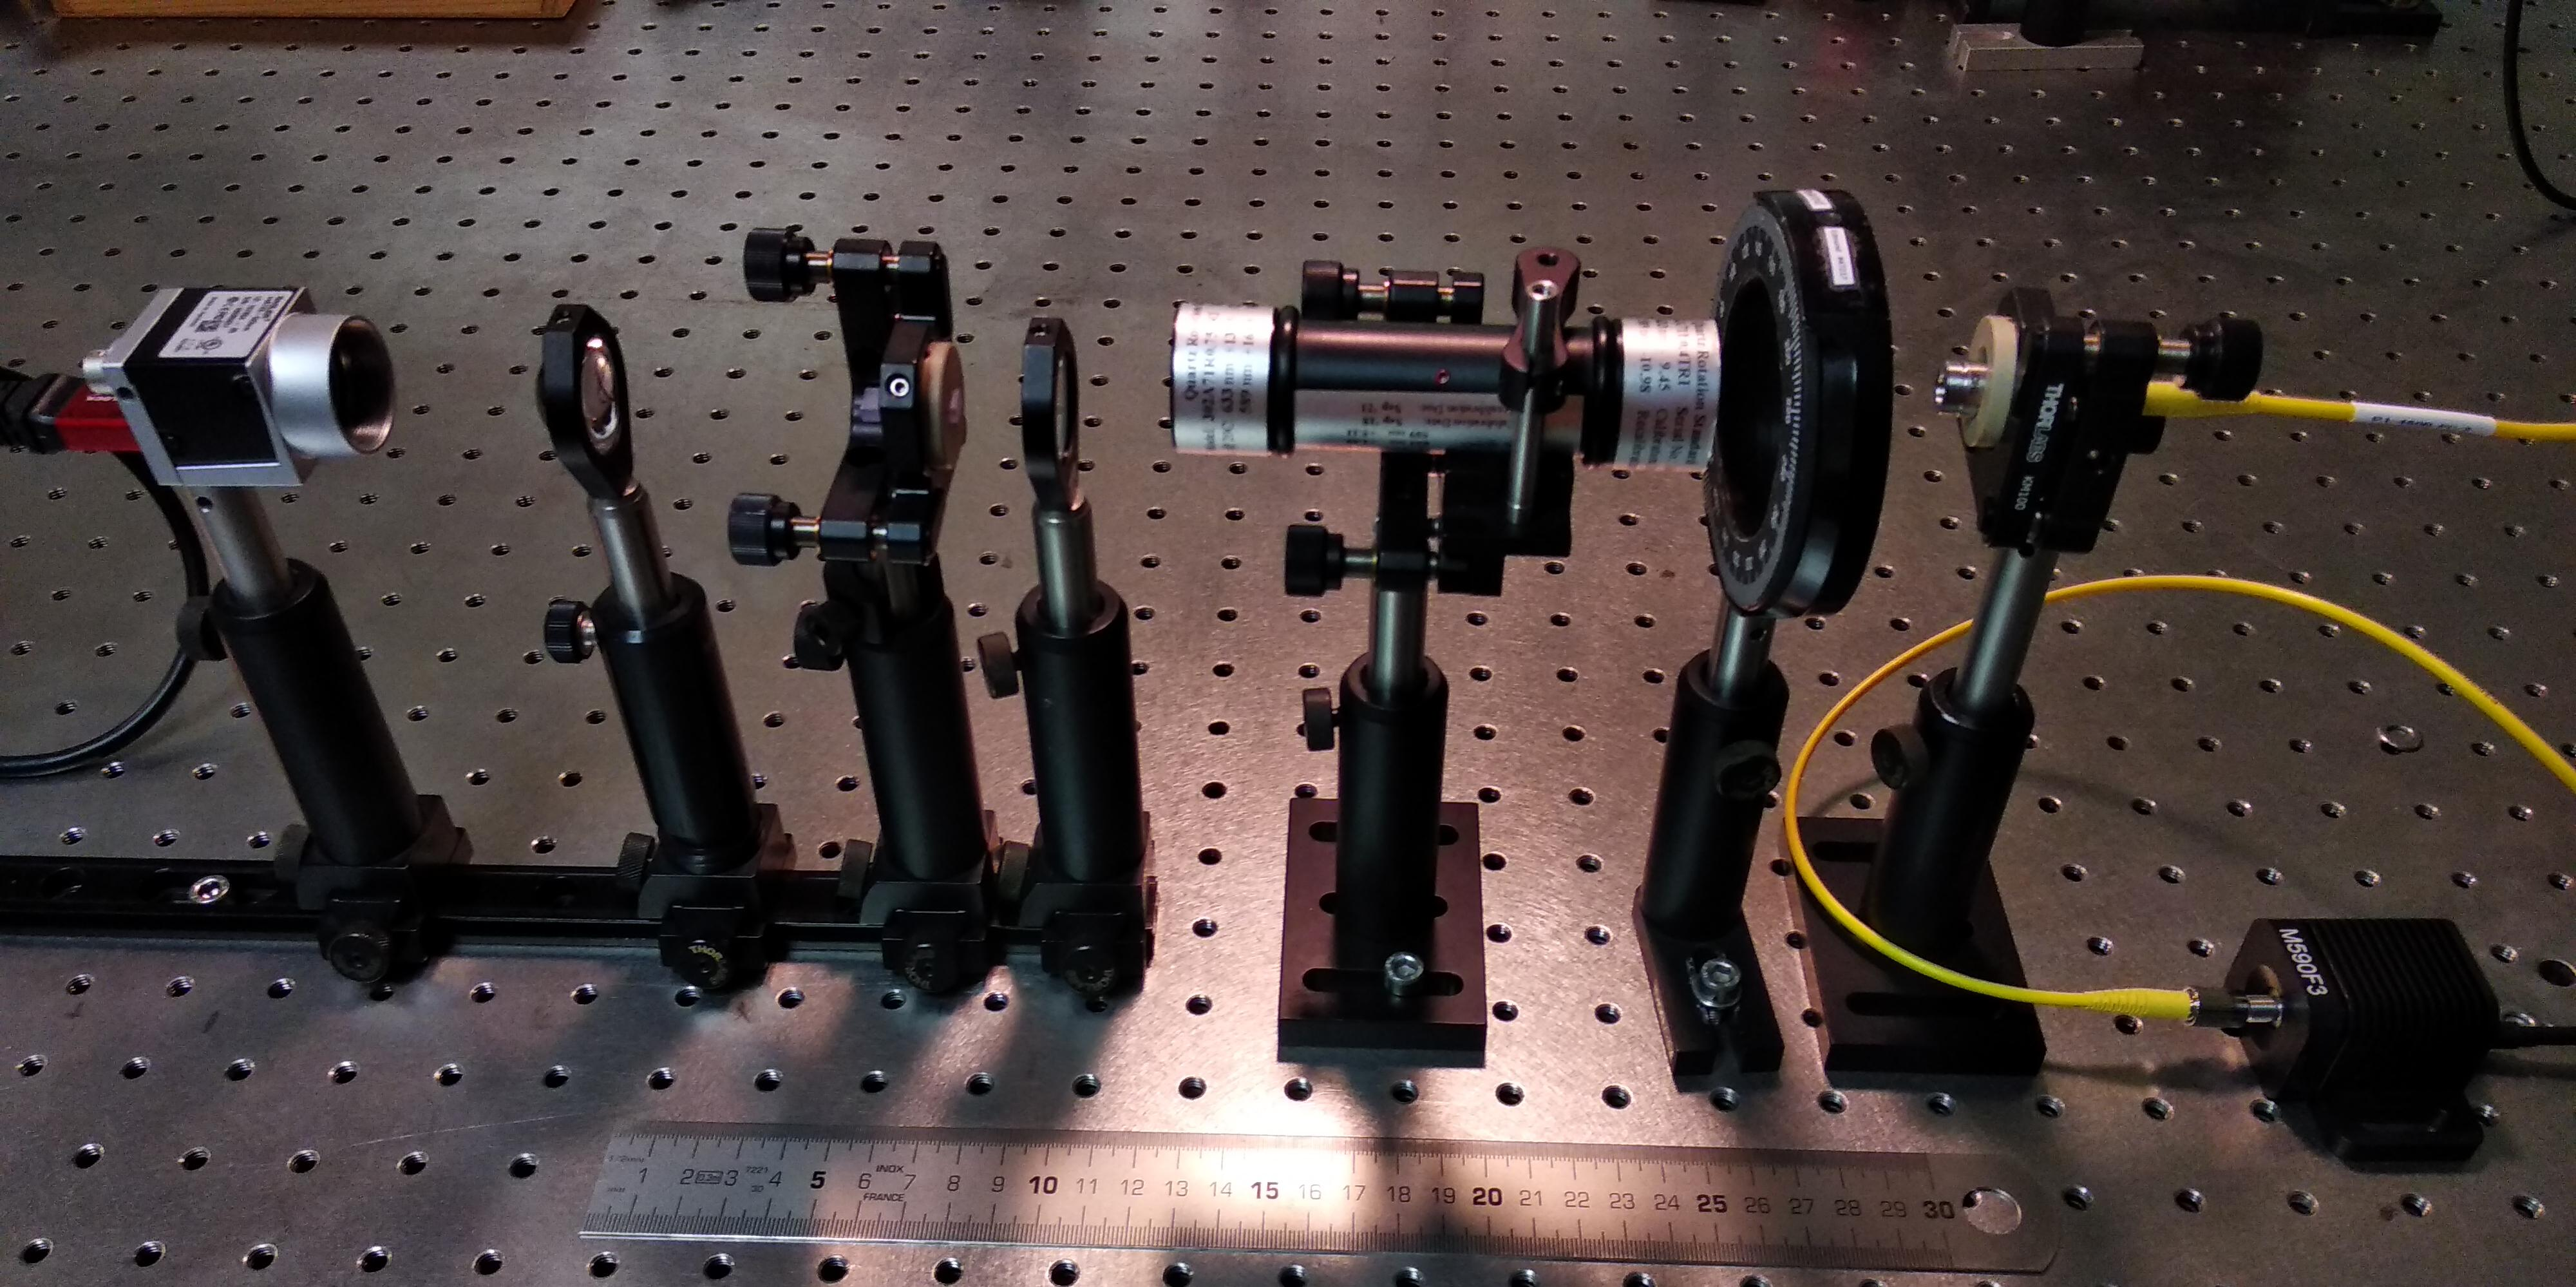
\includegraphics[width=0.55\linewidth]{setup.jpg}
    \caption{ Experimental set-up with the LED M590F3 light source, explained in the text.  }
    \label{fig:track_setup}
\end{figure}


In an alternative set-up, we replaced the light source by an He-Ne laser of 632.8 nm (model Uniphase 1135P, 10 mW), which directly generates a Gaussian profile beam. We placed a light attenuator in its output to reduce its power before it entered to the rest of the set-up.

%\begin{figure}[h!] 
%     \centering 
%    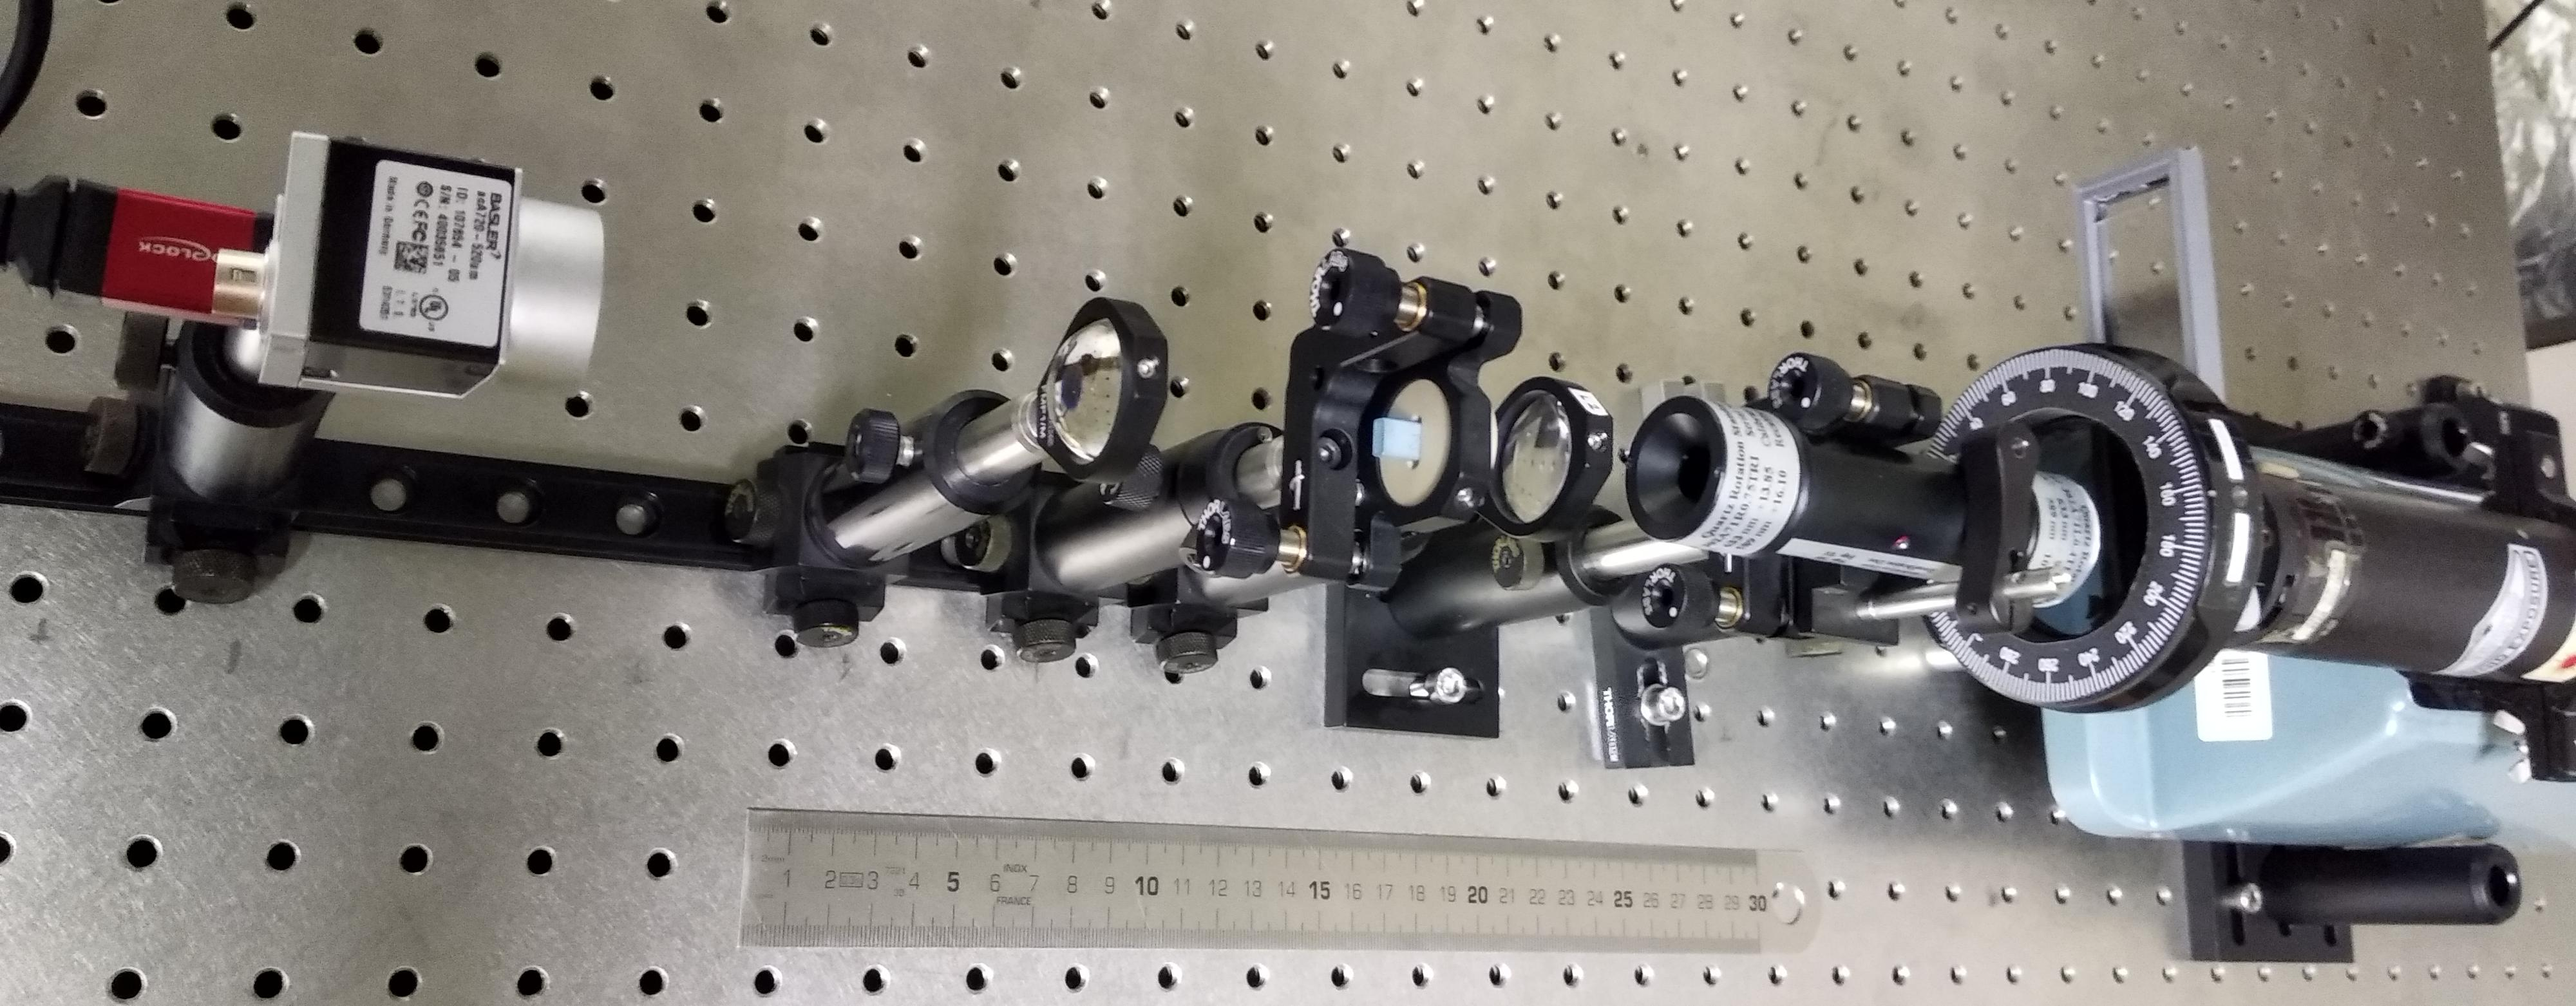
\includegraphics[width=0.5\linewidth]{setup2.jpg}
%    \caption{ Experimental set-up with the He-Ne light source, explained in the text.  }
%    \label{fig:track_setup_alt}
%\end{figure}

The employed crystal for all the work was a monoclinic centrosymmetric $KGd(WO_4)_2$ rectangular prism of sizes $6\times4\times20mm$, with its small faces cut orthogonally to one of the optical axes.\vspace{-0.1cm}

Two different lens settings, causing two different $\rho_0$ were employed. For the LED beam, a first lens (after the light source) of 25 mm focal length and a second lens (for the magnification) of 50 mm were used. For the He-Ne laser, the focal length was 50 mm for the first lens, while 200 mm for the second one.\vspace{-0.1cm}

The employed camera in all experiments was a Basler acA720-520um with a global shutter CMOS sensor of 720$\cross$540 pixels of resolution (6.9$\mu m$ side square pixels). 

%which was collimated coupled to tal, and passed through a single-mode fiber that only allows the passage of the fundamental transversal mode of tal, which has a Gaussian shape. This filtering is done due to the physical restrictions. the reason why we employed a LED array, instead of a laser, which has typically greater coherence lengths, is because .

%
%
%Laser de diodo LED array en una caja que se hace con opticas para ke salga de una fibrita
%https://www.thorlabs.com/thorproduct.cfm?partnumber=M590F3
%
%Fibra single mode apta para la longitud de onda. Single mode fiber.
%
%
%crystal igual que en el articulo.
%
%lentes convergentes de focales 100 lehena 50 bigarrena 
%
%laser de diodo en el poc MC6305C-004S
%
%basler 
%
%
%
%
%
%
% The employed convergent lens 1 has a focal length tal, while the second one has a focal length tal. The employed waveplates on the other hand, where all designed for the same input wavelength.
% 
%The employed camera is a tal with tal
%
%The crystal is tal tal tal.
 
 \fancyhead[OL]{\em Part C: The Body of the Polarimeter}
\fancyhead[OR]{ Setup to Observe Conical Refraction Rings}
\fancyhead[EL]{ Setup to Observe Conical Refraction Rings}
\fancyhead[ER]{\em Bachelor's Thesis: Conical Refraction Polarimeter}
\vspace{-0.2cm}
 
\subsection*{C.1.2. Calibration of the Set-up\vspace{-0.1cm}} 

The most subtle thing to achieve a correct CR ring is to correctly align the light beam with the biaxial crystal. For this we employ a holder for the crystal with two micrometric screws (as can be seen in Figure \ref{fig:track_setup}) that allow us to adjust it in spherical coordinates. This calibration was typically done by visual inspection. The typical approach was to set a $\lambda/4$ wave-plate after the first linear polarizer, in the slot {\bf (c)}, with a $\pi/4$ rad inclination of its main axis relative to the LP of light. This generates a CP light, that should generate a hollow ring in the camera's plane, as we saw in Part A. If the beam is not properly aligned, instead, a sequence of ellipsoids that split up until only two points are visible due to birefringence (when the beam gets very misaligned) can be seen in the camera (see example images in Figure 2.3. of Ref. \cite{Turpin}).

In order to help the manual procedure, three real time image processing methods were designed. The implementation scripts can be found in the project Github \cite{github}, with the rest of generated code.

{\bf Method 1. Analyze the Uniformity of the CP Hollow Ring:} By setting a CP input light, we can pass the images of the camera in real time from Blazquez's Algorithm (B.6.7) to obtain their geometrical centers. Then, by equation \eqref{yoyo}, we know that the angular profile around this center should be a constant when the light beam goes exactly along the optical axis. We fit a line to the angular profile and print in real time the slope of the fitted line. The optimal crystal-beam configuration will be achieved when the slope is closest to zero and visually the ring satisfies the proper intuition. There will always be experimental noise, meaning we will never obtain a flat angular profile. Thus, the RANSAC method \cite{RANSAC} is used to fit the line (instead of a least squares approach), since it allows us to get rid of the outliers that unbalance the line.

{\bf Method 2. Analyze the proximity of the Image to a Simulated Image:} We are able to simulate the perfect theoretical rings that should appear in the camera when the input light beam exactly goes along the optical axis. Then, in real time we can apply the Simulation Fit algorithm of section (B.9) to the captured images, and plot not only the found closest theoretical image to the experimental one, but a similarity metric, like the mean square error between the two images. We can do this both for input LP and CP. Then, we adjust the crystal until the fitted theoretical image has the least possible mean square error.

{\bf Method 3. Analyze the Proximity of the angular profile to a Squared Cosine:} From equation \eqref{cosine} we know that for input LP, when the light beam goes along the optical axis, the intensity profile about the geometrical center should be a cosine squared. Then, by setting an input LP, we apply in real time the Blazquez+RANSAC cosine fit algorithm of section (B.6.9), which will show us the angular intensity profile along the geometrical center of the ring, together with the best RANSAC cosine square fit. We adjust the crystal until the generated profile has a minimum fit error.

The procedure could be improved even more if we had an electronic component to control the crystal adjustment with a computer. If so, we would simply apply a 2D optimization algorithm like the ones described in part B, on the degrees of freedom moving the crystal.
\vspace{-0.2cm}


\section*{C.2. Non-Idealities in the Experimental Rings \vspace{-0.15cm}}
\addcontentsline{toc}{subsection}{2. Non-Idealities in the Experimental Rings}
\fancyhead[OR]{ Experimental Ring Non-Idealitites}
\fancyhead[EL]{ Experimental Ring Non-Idealitites}
As can be seen in Figure \ref{fig:expnoise}, experimental images, even the ones taken with care to build the test datasets, present notable noise, breaking the theoretical assumptions not only about the background, but especially about the predictable intensity profile of the rings. We can see in these images that essentially not even a single symmetry of those listed in (B.1) is fulfilled. Yet, we expected the quality and robustness of the algorithms to be enough to render the effect of noise at least for an interesting resolution, which turned out to be the case.\vspace{-0.1cm}

Let us list the main noise sources we encountered and how we managed to partially solve them:\vspace{-0.25cm}
\begin{itemize}
\item Each camera pixel sensor, in the end, is counting the number of light energy packages (so called photons) that arrive to it. These arrivals happen randomly, but ideally, each pixel should detect an expected number of photons per unit time, proportional to the intensity of the electric field. These are essentially the assumptions of the Poisson model, as derived in Ref. \cite{poisson}. The random variable for the photon count in each pixel $V_{x,y}$ then follows a Poisson distribution $V_{x,y}\sim Poiss(\lambda=\alpha I(x,y))$, with $I(x,y)$ the deterministic pattern without this count-noise and $\alpha>0$. Such a noise can be diminished by averaging over $N$ images $I_k\sim V^{(k)}_{x,y}$. This is because without changing the experiment, images are independent random samples of the identically distributed $V^{(k)}_{x,y}$. Then $I_{average}=\sum_{k}V^{(k)}/N$, meaning the variance on each pixel is reduced by a factor $N$: $var_{x,y}[I_{average}]=\sum_k var[V_{(x,y)}^{(k)}]/N$, where $var[V_{(x,y)}^{(k)}$] is constant, while the expectation is still the same $E[I_{average}]=E[V_{x,y}^{(k)}]=I(x,y)$. Thus we get an improved signal to noise ratio. Note that for the interpretation as photon counts, averaging is equivalent to increasing the exposition while avoiding the pixel saturation, which is an alternative solution.

\item If the optical fiber from which the laser is outputted allows the passage of other modes than the Gaussian one, the shape of the generated rings need not be equal to the ones we solved in (A.3). This can be easily solved with a single-mode fiber for the particular wavelength, that due to physical constraints avoids the passage of higher order Laguerre-Gaussian modes that solve the paraxial Helmholtz equation in cylidrically symmetric coordinates. Alternatively, employing other techniques to light the crystal, that lead to similar rings (like placing a pinhole after the source), are considerable solutions. \vspace{-0.1cm}

\item If the transversal intensity profile of the beam that arrives to the crystal is not cylindrically symmetric (even if it is a Gaussian), the waist will not be homogeneous along the ring. Since this pattern does not rotate with the polarization plane, it breaks the main axis symmetry.
\item If in the calibration process we use a waveplate, to generate CP, that is not exactly designed for the input wavelength, then it will be elliptically polarized instead of circularly. Then, the calibration can be done wrong, leaving un-homogeneous waists for the ring (misalignment with the optical axis).

\item If there are imperfections in the optical elements or there are dust particles, strange diffraction patterns may emerge, that will make the crests of the conical refraction ring be wavy. 
\item The crystal or the protective glass of the camera's eye may have double reflections in their walls, that can generate several dimmer rings inside the main one.\vspace{-0.2cm}
\end{itemize}
Even if a careful calibration should avoid these noises, with the budget limitation of a low-cost device, we find it hard to avoid the fluctuations on the crests of the rings, as well as the non-homogeneity of the waist of the ring. These are clearly appreciable in Figure \ref{fig:expnoise}. Thus, these two, together with the pixel-wise
Poisson noise are the factors we try to model with the artificial noise in (B.2).\vspace{0.1cm}
\begin{figure}[h!] 
     \centering 
    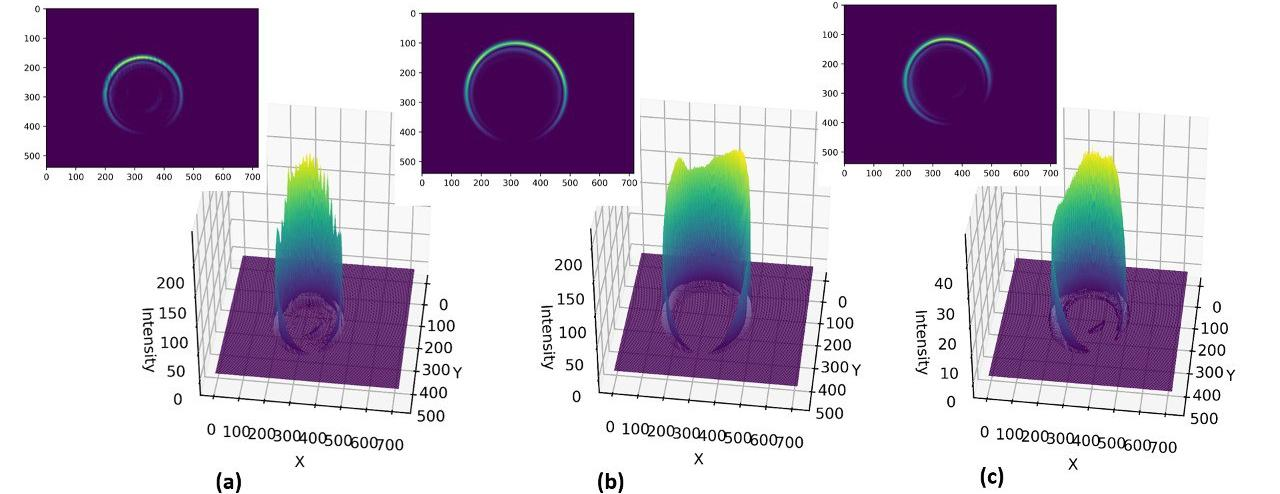
\includegraphics[width=\linewidth]{exp.jpg}
\caption{Example experimental images as colormaps and surface plots. (a) Image of the He-Ne dataset. (b) Image taken in the LED source setup. (c) Image of the LED dataset. }
        \label{fig:expnoise}
\end{figure}
\vspace{-0.5cm}
\section*{C.3. The Experimental Image Dataset\vspace{-0.1cm}}
\addcontentsline{toc}{subsection}{3. The Experimental Image Dataset}
\fancyhead[OR]{ Experimental Image Datasets}
\fancyhead[EL]{ Experimental Image Datasets}
In order to benchmark the designed algorithms (of part B), it is important to have CR crescent ring image pairs labeled with their ground-truth $\Delta \Phi_{LP}$. An option for this is to employ another polarimeter with a higher resolution and precision than the one we intend to build. This would allow us to generate a big labeled dataset. Since we had no other polarimeter, this was not an option.

What we could obtain was a certified sample (by DigiPol Technologies) with two crystals that each rotate the linear polarization plane a certified number of degrees (with a precision of $\pm 0.01$ deg), labeled both for a wavelength of 633 nm and 589 nm (this is in part the reason why we employed the two set-up light sources). With this, for each of the input light beams, we can generate four different crescent CR rings with a known pair-wise $\Delta \Phi_{LP}$: a total of 6 different reference-problem pairs. Then, for each set-up we got an additional pair: using two linear polarizers, we can rotate them relatively until they extinguish the output light. At that point the polarizers have their axes orthogonal to each other, meaning they only leave light through at a relative polarization of $\Delta \Phi_{LP}=\pi/2$ rad.

With all, we built two labeled experimental image datasets of 7 sample-pairs, that can be employed for the final test of the algorithms. Examples of these images can be found in Figure \ref{fig:expnoise}.	\vspace{-0.35cm}

\subsection*{C.3.1. Results of the Algorithms on the Experimental Datasets}\vspace{-0.05cm}
Running the same pipeline of (B.10.1) on the experimental datasets, we get the results that can be found in the {\em /RESULTS} folder of the repository \cite{github}.
%\vspace{-0.02cm}

\begin{table}[h!]
\center
\caption{Sumary of the best variant found for each algorithm on the HeNe laser dataset. Confidence intervals are not shown, since with only 7 samples, they are not significant enough. Std stands for standard deviation. }\label{tab:resExp}
\hspace{-0.1cm}\begin{tabular}{c|c|cc|cc}
\toprule
 \multicolumn{2}{c|}{\bf Algorithm} &  \multicolumn{2}{|c|}{\bf \small Abs. Error (rad)} & \multicolumn{2}{|c}{\bf Times (s)} \\ \midrule \midrule
{\bf                     Name} &                          {\bf Winner} {\bf Variant} &  {\bf Mean} &  {\bf Std.} & {\bf Mean} & {\bf Std.}\\
\bottomrule\rule{0pt}{4mm}{}
    Cosine squared fit &  {\small  Opt. Nelder-Mead, final estimation } &  0.50(5) &  0.29 &  2.88 &  0.012 \\
                       &                   {\small using RANSAC+cos fit }&          &         &          &          \\ \hline\rule{0pt}{4mm}{}
               Blaquez &  {\small  Opt. Nelder-Mead, final estimation } &  0.51(7) & 0.43 &  0.52 &  0.020 \\
                       &                   {\small using RANSAC+cos fit }&          &         &          &          \\ \hline\rule{0pt}{4mm}{}
   Blazquez+Cosine Fit &              {\small w=0.999, Opt. Nelder-Mead} &  0.52(4) & 0.32 &  3.43 &  0.041 \\ \hline\rule{0pt}{4mm}{}
    Polar Registration &     {\small      Preproc. Sigmoid k=35, c=0.3} &  0.54 & 0.54 &  0.26 &  0.011 \\ \hline\rule{0pt}{4mm}{}
           Mirror flip &     {\small    Opt. Quad., Bicubic Interpol., }&  0.56 & 0.41 &  0.14 &  0.0080 \\
                       &        {\small   Preproc. Sigmoid k=35, c=0.3 }&          &         &          &          \\ \hline\rule{0pt}{4mm}{}
  Kalkandjiev-Rotation &      {\small  Opt. Fibo., Bicubic Interpol.,}  &  0.57 & 0.42 &  0.22 &  0.020 \\
                       &          {\small Preproc. Sigmoid k=35, c=0.3 } &          &         &          &          \\ \hline\rule{0pt}{4mm}{}
        Simulation Fit & {\small About Gravic., Opt. Nelder-Mead,}  &  0.58 & 0.39 &  1.57 &  0.042 \\
                       &                  {\small Preproc. Norm. to Max }&          &         &          &          \\ \hline\rule{0pt}{4mm}{}
     Relative Rotation &    {\small     Opt. Quad., Bicubic Interpol.}, &  0.61 & 0.45 &  0.069 &  0.0080 \\
                       &      {\small     Preproc. Sigmoid k=35, c=0.3 }&          &         &          &          \\ \hline\rule{0pt}{4mm}{}
                       
       Simulation Fit + &    {\small     Opt. Quad., Bicubic Interpol.}, &  0.88 & 0.52 &  2.17 &  0.033 \\
   Embedder                    &      {\small     Preproc. Sigmoid k=35, c=0.3 }&          &         &          &          \\ \hline\rule{0pt}{4mm}{}                     
                       
     Bimodal Histogram &       {\small    Preproc. Sigmoid k=35, c=0.5 }&  1.48 & 1.59 &  0.14 &  0.0025 \\ \hline\rule{0pt}{4mm}{}
Gravicenter Regression &         {\small  Preproc. Sigmoid k=35, c=0.3 } &  2.20 & 1.96 &  0.48 &  0.017 \\ \hline\rule{0pt}{4mm}{}
          KNN+Embedder &                {\small UMAP Embedder, Trained } &  2.76 & 2.05 &  3.33 &  0.0 \\
                       &                      {\small on Non-Noisy Data} &          &         &          &          \\ \hline\rule{0pt}{4mm}{}
                   KNN &    {\small  Trained w. (simulated) Noisy Data }&  4.23 & 2.64 &  1.80 &  0.0 \\
\bottomrule
\end{tabular}

\end{table}
\vspace{0.07cm}
In Table \ref{tab:resExp}, we gather the best algorithm configurations found for the HeNe light source dataset. As it can be seen, the results are significantly better than those we found for the noisy simulated images. Interestingly, we see that for this intermediate noise level, we find an alternative oredering of the algorithms. It is important to note however, that since the ground-truths are only precise to the second decimal place, in reality the three first algorithms in the table perform equally well in terms of mean absolute error. Having this in mind, the best alternative, even though it has the highest standard deviation, seems to be the Blazquez algorithm, since its computation time is six times smaller than the other two. Note that the ordering in reality is not that surprising, because these first three are closely followed by the Kalkandjiev, Mirror and Simulation Fit algorithms. This means the trend follows an intermediate rationale to the results in the highly noisy and ideal simulated datasets as seen in (B.10.1). The rest of conclusions are akin to the ones in the analysis of (B.10.1).\vspace{-0.06cm}

For the LED dataset (see the repository), we find that the best algorithm is also the Blazquez algorithm, with a mean absolute error of 0.53 deg and a standard deviation of 0.26 (closely followed by the Kalkandjiev and Mirror algorithms).\vspace{-0.06cm}

Considering these results and those in (B.10.1), we can conclude that since depending on the noise level present in the images, the best algorithm turns out to a different one, a full benchmark should be run to know the optimal strategy for any new set-up. This proves the convenience of having developed an extensive algorithm pool, based on different features of the images.
\newpage

\section*{C.4. The Polarimeter, a Proof of Concept\vspace{-0.1cm}} 
 \addcontentsline{toc}{subsection}{4. The Polarimeter, a Proof of Concept}
 \fancyhead[OR]{ The Polarimeter, a Proof of Concept}
\fancyhead[EL]{\ The Polarimeter, a Proof of Concept}
We can naturally suggest following the discussion of (A.4), the experimental setting of (C.1) and all the algorithms of (B), a device that measures changes in the linear polarization of light. Such a device could have two different configurations: rather the input to the device is the light beam itself, or the device already has a light source and the input is a sample changing its polarization. The first option would be the convenient one for instance for the detection of exoplanets using LP light \cite{exoplanets, exoplanets2}. The second one would be the convenient one for the pharmaceutical enantiomerism or optical concentration measurements of the food/berverage industry, as commented in (A.4). In fact, this second configuration is the one found most typically in a laboratory, which if it only requires the user to input the sample and wait for the results, is commercially knwon as an {\bf automatic polarimeter}. Because in this option, the light beam and its parameters, which affect so critically to the conical refraction phenomenon, are under our control, we decided opted for such a configuration, following the prototype built in Ref. \cite{incomplete} by Lizana {\em et al}.

By now it is clear that device will have three parts of different nature: an {\em optical part} with the components described in (C.1); an {\em electronic part} encompassing both the camera and the computer to convert the images into meaningful information; and, the main merit of the present thesis: the {\em algorithmic part}, that will rule the measurement of the polarization and will interact with the user. With this scheme, let us present in Figure \ref{fig:proof} the proof-of-concept of the device made for the thesis.

Its specifications are the following ones:\vspace{-0.15cm}

{\bf $\bullet$ Optical Part:} A LED M590F3 - 590 nm 3.3 mW ligth source, coupled to a single-mode fiber and a collimator, consuming 3V at 950mV. A convergent lens with 100 mm focal length. A monoclinic centrosymmetric $KGd(WO_4)_2$ rectangular biaxial crystal of sizes $6\times4\times20mm$.\vspace{-0.1cm}


{\bf $\bullet$ Electronic Part:} A Basler acA720-520um camera. A Raspberry Pi 4 mini-computer with 4Gb of RAM. A Raspberry Pi 3 7'' Touchscreen Display for user interaction with the computer.\vspace{0.2cm}

\begin{figure}[h!] 
     \centering 

    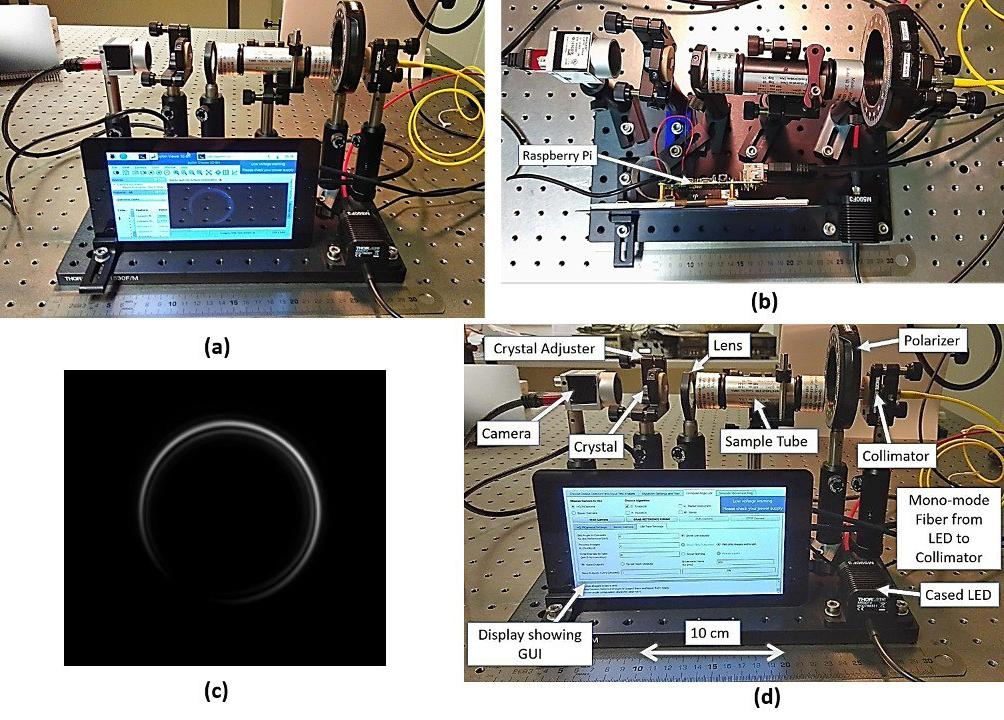
\includegraphics[width=0.88\linewidth]{demo.jpg}
\caption{The proof-of-concept polarimeter. (a) Frontal view. (b) Superior view. (c) Image taken by its camera and part of the proof-of-concept dataset. (d) Details of the components of the prototype.}
        \label{fig:proof}
\end{figure}

{\bf $\bullet$ Algorithmic Part:} A graphical user interface (GUI) application, programmed using Python and the PyQt library \cite{pyqt} with all the algorithms of part B available within it, allowing the user to fully customize their parameters. The dependencies and a small manual, together with all the code can be found in the project Github repository \cite{github}. Essentially, it allows: (a) the determination of $\Delta \Phi_{LP}$ for two particular takes; (b) a continuous real-time monitoring of $\Delta\Phi_{LP}$ (relative to an initial reference LP); (c) the simulation of theoretical images. The touchscreen in Figure \ref{fig:proof}.d is showing this GUI application.



Note that we have placed no magnification of the ring prior to the camera, which means the images that will be captured will have a lower resolution than those with which we worked in the rest of the work (the image in Figure \ref{fig:proof}.c has 170$\times$160 pixels, against the 540$\times$720 of the ones in Figure \ref{fig:expnoise}). In part this was because in the basis of the device there was not enough space for that. Yet this is not the only reason, for it could be solved by placing a mirror in the corner where the camera is, and placing the camera in the next corner, to allow the addition of a second lens (requiring a lengthen optical path). The main reason was that we decided to stick to a simpler configuration to make the device robuster to noise and to de-calibration. Even if the resolution is smaller, using a lens less introduces much less noise in the images and the device is simpler to be calibrated and harder to be de-calibrated by accidental hits. Moreover, if the final version is to include the Pi camera with a higher pixel density, as we explain in the next section, the magnification will not be needed at all.\vspace{-0.1cm}

\subsection*{C.4.1. Proof-of-concept Dataset and Algorithm Check \vspace{-0.1cm}}

We generate a small labeled dataset following the same steps as for (C.2), now employing the proof-of-concept. We use it for testing the algorothms using the pipeline explained in (B.10.). The full results can be found in \cite{github}, but the main highlights are the following ones:\vspace{-0.2cm}
\begin{itemize}
\item The best algorithm for the proof-of-work turns out to be the Simulation Fit algorithm, using the geometric center fix, preprocessing the images to the mean value and using the Nelder-Mead optimizer. It gives a mean absolute error of $0.72$ deg with a standard deviation of 0.45 deg. The average time taken per image is of 0.36 s.\vspace{-0.1cm}

\item It is followed by the Kalkandjiev-Rotation algorithm (B.6.3.) with the Quadratic Fit search algorithm and using cubic interpolation. It gives an average absolute error of $0.81$ deg and a standard deviation of $0.74$ deg. The average time taken per image is of $0.07s$.\vspace{-0.3cm}
\end{itemize}

These resulting precisions are comparable to those obtained with the full magnified ring set-up in (C.2), so we can consider the hand-made low-cost prototype to be a success.\vspace{-0.1cm}

\subsection*{C.4.2. Cost Analysis\vspace{-0.1cm}}
We can estimate an upper bound of the production cost of the device by the cost of its components in the general customer market. See a summary in Table \ref{tab:prices}. Note that if the device was mass produced the price of the components would drop significantly. 


Notice that we assume that all the casing and support materials could be made using a 3D printer, with all the optical elements readily aligned and an adjustable part to calibrate the crystal's orientation. This casing would protect and fix all the components, only leaving an opening to introduce the sample and the access to the touchscreen.

Very importantly, note that we do not require all the features offered by the Basler camera (like the 525 frame per second rate), such that for example the High Quality Pi Camera of Raspberry would be enough. This second camera is sold for 50 euro (Farnell) and has actually a bigger resolution (12.3 MP) than the Basler camera, meaning higher precision measurements would be obtained. This is not only for the increase in the number of pixels, but is especially due to the fact that its pixels have a smaller pitch of 1.55 $\mu m$ (compared to the 6.9 $\mu m$ sized Baselr pixels), which means that possibly without magnification the same effective resolution as the test images of set-up (C.1) could be obtained. \vspace{0.1cm}
\begin{table}[h!]
\caption{Table with the general customer rounded prices of the components of the proof-of-concept. }
\centering
\label{tab:prices}
\begin{tabular}{c|c|c}
\toprule
    {\bf Component}& {\bf Vendor } & {\bf Price (euro) } \\
\hline
Polarizer film & Thorlabs & 9\\
3V 1A Power Supply for light source & Amazon & 10\\
Lens 100 mm & Thorlabs & 19\\
Casing and element support 3D printer material & Estimated & 50 \\
Raspberry Pi 4 & Amazon & 40\\
Raspberry Touchscreen 7'' & Farnell & 50\\
Single-mode fiber apt for 590 nm & Thorlabs & 72 \\
Biaxial crystal cut in the right crystalographic plane & Altechna (priv. comm.) & 300 \\
LED M590F3 - 590 nm 3.3 mW & Thorlabs & 430\\
Basler acA720-520um camera & Basler & 330\\
\hline
Total & - & 1310 \\
\bottomrule
\end{tabular}
\end{table}
%Moreover, the LED light source can also be hand-made using for instance the Nichia: NCSAE17A LED and a hand-made printed case and fiber coupling, which would drop the price of the device even more.

Let us leave the component price at 1010 euros (for the substitution of the Basler camera by the Pi camera). Then, once the case is printed, by considering that mounting the device, callibrating it and installing the necessary dependencies and software, takes about 2 hours, if we assume a 30 euro/h handwork: we could get a fully operational automatic polarimeter based on the proof-of-concept by 1070 euros. This would then be the upper bound of its production cost.\vspace{-0.1cm}
\subsection*{C.4.3. A Comparison with Commercial Automatic Polarimeters }

\subsubsection*{Qualiltative Comparison \vspace{-0.1cm}}
Commercial automatic polarimeters work in a very different way to ours \cite{polarimeters}. They have a mechanically movable linear polarizer and an intensity measuring device after-wards. The polarizer is rotated from a fixed initial position until a maximum intensity angle is found (or the no intensity angle, which by orthogonality also indicates the direction of polarization). Then, for the next sample, the linear polarizer goes back to its initial position and a new measurement is taken. The relative angle $\Delta \Phi_{LP}$ is given by the difference in the rotation of the polarizer. The precise measurement of this rotation is typically done using chains of gears (or similar components) that can rotate the linear polarizer by a fixed angular amount. Essentially, this amount gives the precision of the polarimeter. Clearly it is a very robust technique for its simplicity, but it has its own drawbacks. On the one hand, the mechanical setting makes the device have a considerable weight and dimensions. Most importantly however, the need to move a mechanical setting and to take measurements in each small displacement makes the device require as much as a few seconds for the maximum precision in each measurement (we will see that even the fastest polarimeters require at least 1 second). This means a real time monitoring only offers a maximum of a single measurement per second, which might be pointless for kinetic constant determination in fast chemical reactions. In addition, the precision of the measurements is bounded by how small the displacements are feasible to be made mechanically, given they should be done in a reasonable time and the device should occupy a reasonable space. 

In contrast, our device is a "snapshot" polarimeter, which only requires to take a photo and process it to obtain all the information about the polarization. This is because the CR phenomenon naturally acts as a continuous set of linear polarizers in all possible orientations. At a single time, it gives us the amount of light that each possible linear polarizer would allow to pass in each angular position. The limitation of course, is that the digitalization must be done with a discrete pixel array. Yet it is true that, this transferral of the mechanical problem into a digital one not only means the importance is now placed in the algorithms to resolve the computer vision task, but especially means the resolution with which we can discern a variation of the angle, is not limited by the physics of the gears, but by the resolution density of the camera taking the image (which unfortunately is quite poor for our camera). In contrast with the finer gear development, it is well known that the camera industry is developed independently of the polarimetry industry, meaning the precision of the device would benefit "for free" from the progress made by such a powerful sector.\vspace{-0.1cm}

\subsubsection*{Quantitative Comparison \vspace{-0.1cm}}

In Table \ref{tab:commercial}, we have gathered some commercially available automatic polarimeters. As it can be seen, these polarimeters offer a better precision than our proof-of-concept. Yet, none of the precisions is better than our achievable precision (as seen in the tests in B.10.); which could in principle be attained by increasing the resolution of the taken ring images, by reducing the noise with better quality optical components or a more precise alignment using a 3D printed mould, and by calibrating the crystal's orientation with electronic control.\vspace{0.1cm}
\begin{table}[h!]
\caption{Some commercial automatic polarimeters sold in 2022 by IRMECO, a German laboratory supplier. }
\centering
\label{tab:commercial}
\hspace*{-0.4cm}\begin{tabular}{c|c|c|c|l}
\toprule
{\bf Polarimeter Brand} & {\bf Price } & {\bf Accuracy} & {\bf Source} &{\bf 	Features}\\
{\bf and model} & {\bf (euro)} & {\bf (deg)} & \\

\midrule
Krüss Polarimeter & 8,150 {\footnotesize + VAT} & $\pm 0.01$ & LED 589 nm & - Fast Meas. time $\sim 1s$\\
P3000  & & & & - Thermometer\\ Cat. N. 10 61 13000 & & & & - 28 kg; 645 x 200 x 360 mm\\ \hline\rule{0pt}{4mm}{}
Krüss Polarimeter & 12,247 {\footnotesize + VAT} & $\pm 0.003$ & LED 589 nm & - Fast Meas. time $\sim 1s$\\
P8000 & & & & - Thermometer \\ Cat. N. 63 61 80000 & & & & - 28 kg; 645 x 200 x 360 mm\\ \hline\rule{0pt}{4mm}{}
Krüss Polarimeter & 22,544 {\footnotesize + VAT} & $\pm 0.002$ & LED 589 nm & - Fast Meas. time $\sim 1s$\\
P8100-TF  & & & & - Thermometer \\
Cat. N. 10 61 18104 & & & & - Sample temperature control\\
& & & & - Flow through and drying unit \\ & & & & - 28 kg; 645 x 200 x 360 mm\\ \hline\rule{0pt}{4mm}{}
 Schmidt\&Haensch & 18,360 {\footnotesize + VAT} & $\pm 0.005$ & LED & - Two fixed wavel. to choose\\
  Polartronic V& & & & in {\small $\{405, 435, 546, 578, 589, 633, 882\}$}\\
  201 SC & & & & - Thermometer\\
    & & & & - Meas. time $\sim 4s$ \\
    & & & & - 18.3 kg; 730 x 370 x 160 mm \\

 \bottomrule
\end{tabular}

\end{table}


Following the previous qualitative observations, we can note several points in comparison with our device, to layout the potential niches it could cover:
\begin{itemize}
\item The measurement times are in all cases slower than in our device. In fact, all these Krüss polarimeters belong to a same assortments of automatic polarimeters, which according to their manual \cite{manual}, from 2003, when they patented the fast measurement protocol (until at least 2016, the date of the manual), {\bf "are the fastest" automatic "polarimeters in the world"}. And they are an order of magnitude slower than ours (in its preliminary version). Then, a potential target for our polarimeter could be the sector needing fast real-time polarization measurements. These presumably include the chemistry community employing polarization measurements for non-invasive concentration monitoring to get the kinetic constants of chemical reactions.

\item They are all considerable in size and weight, as opposed to our device. In its current version our device weights about 2 kg (which can be made lighter using the 3D printed casing and holders) and measures 150 x 200 x 300 mm, which can be reduced a half in the vertical axis of 200 mm, by setting the optical components in the same height as the display. Moreover, since as power input, we only require to feed the LED and the Raspberry Pi, a portable rechargable battery could be installed. This means our device could potentially also target the customers that prefer a portable and lightweight version of the device. Such an example could be University teaching laboratories or field researchers.


\item They all include a thermometer and some include sample temperature control devices or tubes and extra components to allow live flow of samples through the device instead of using a static tray. The thermometer is not an expensive component, so it could easily be implemented in our device. When it comes to the rest of components, we see that they include them at the cost of about 10,000 euro (comparing the second and third model of the table, which are the same otherwise). With this difference, we could presumably include them as well.

\item Finally, the prices of the polarimeters are significantly bigger than the production cost of our device, even in its home-made version. Since any customer prefers a cheaper device, this is a hook for any potential client.
\end{itemize} 

With all, even if there are many points which must be improved for a fully functional and competitive prototype, our device seems to allow many possible specializations to fit the different niches we described.


\newpage
\fancyhead[L]{\null}
\fancyhead[R]{\null}
%\null
%\clearpage











\section*{\centering \huge{ Conclusions and Future Work}\vspace{-0.44cm}}
\noindent\rule{\textwidth}{0.4pt}

\addcontentsline{toc}{section}{Conclusions and Future Work}

In a nutshell, using the theoretical properties of CR, we have developed a considerable collection of algorithms to predict the linear polarization of light given a CR crescent ring image. We have tested them against theoretical simulated images with and without noise, and against experimental labeled images. We have obtained an experimental precision of $\pm 0.5$ deg, with an ideal obtainable precision of $\pm 0.001$ deg using the same camera resolution. Both of them shall improve significantly with the use of a camera with smaller pixels (thus, higher resolution for the same rings). We have then crafted a low-cost proof-of-concept automatic polarimeter and tested the algorithms on it, to obtain a precision of $\pm0.7$ deg. The difference was mainly due to the fact that we omited the magnification step to reduce lens noise and to give robustness to the device. Both of these results are nevertheless already better than the previously reported CR polarimeter in Ref. \cite{incomplete}, where a precision of $2.6$ deg was obtained. We have also analyzed the market of automatic polarimeters and have seen that our device has a big potential to compete with top sold (and expensive) polarimeters. We have proposed several directions into which we could continue building prototypes, from a more expensive one trying to refine the procedure to the maximum, to an even cheaper, more versatile and portable one, which would at least have the precision of our handmade prototype.\vspace{-0.07cm}

Aside exploring all the ideas towards the improvement of the proof-of-concept, it is left as a future work to test which is the limit in the obtainable precision by only increasing the pixel density of the camera. If the rest of optical setting is refined into industrial accuracy (avoiding a handmade process as ours), this could mean the device has the potential to be the most precise of the automatic polarimeters. This is a serious consideration because the phenomenon, in theory, offers an infinite degree of precision in a single image, only spoiled by the experimental noise and the necessary discretization of a camera-sensor. When it comes to the algorithms, the deep learning approach to the problem still needs to be thoroughly explored. Also, it is left as future work to test whether the extension of the Blazquez algorithm suggested in section (B.6.7) could really lead us to a groundbreaking algorithm. \vspace{-0.07cm}

All in all, if there is a message to be learned from this work, it is that although it was tabled almost 200 years ago, the beautiful proof of the mighty  power of mathematics by Fresnel and Hamilton, known today as conical refraction, has still an endless potential to be unchained.
%\BgThispage

\vspace{-0.15cm}

\subsection*{Acknowledgments \vspace{-0.15cm}}
I would like to thank Alex Trupin for all those hours in the lab calibrating Concical Refraction rings, for all his advice and invaluable help. Thanks for all the patience you have had with my clumsiness in experimentation, for answering all my questions and requests for finner and finner rings. Thanks for explaining me once and again the essentials and tricks of an optics laboratory. You have gave me an invaluable knowledge. {\em Per aquesta aventura i per totes les que vinguin!}\vspace{-0.05cm}

Thanks a lot to Jordi Mompart, who was the one who opened me the door (once again) to such an interesting project. Thanks for all the trust you place on me in every adventure we share! {\em Jamás podré agradecerte lo suficiente}. Hope the work is up to your expectations! \vspace{-0.05cm}

Thanks to Carles Blazquez for his inestimable contribution to the algorithms. It turns out your algorithm is one of the robustest! {\em ¡Quizá algún día descubras el color del cielo de uno de los exoplanetas que estudias con tu propio algoritmo! ¡Espero estar ahí cuando suceda!}

And of course, my deepest gratitude to Todor Kirilov Kalkandjiev. An exemplary scientist and professor, and an even greater person, who I admire and is for me a reference who showed me that it is possible to live with this love towards the {\em thaumazein}, the fascination in front of this world, until the last one of our days. I wish you could see the results of your project and we could continue the path towards the device you had in mind. This work is because of you, and is entirely for you.\vspace{0.1cm}\newline {\em Sí, me debes una caña };)



\newpage

\fancyhead[OL]{\em Conclusions}
\fancyhead[OR]{ }

\fancyhead[EL]{\em }
\fancyhead[ER]{\em Bachelor's Thesis: Conical Refraction Polarimeter}

\newpage
\fancyhead[OL]{}
\fancyhead[OR]{}
\fancyhead[EL]{}
\fancyhead[ER]{}
\null



\newpage
\begin{thebibliography}{1}
\addcontentsline{toc}{section}{References}
{\small 
\bibitem{LL}
L. D. Landau and E. M. Liftschift. {\em Electrodynamics of Continous media.} 2nd Edition. (Oxford, 1960)

\bibitem{magnetostatic}
D. D. Stancil. {\em Theory of Magnetostatic Waves}. Springer New York (1993).

\bibitem{fundamentals}
B. E. A. Saleh and M. C. Teich. {\em Fundamentals of Photonics}. New York Wiley. (1991)

\bibitem{BK1}
A. M. Belskii and A. P. Khapalyuk. {\em Internal conical refraction of bounded light beams in biaxial crystals.} Opt. Spectrosc. 44, 436 (1978).

\bibitem{BK2}
A. M. Belskii and A. P. Khapalyuk. {\em Propagation pf confined light beams along the beam axes (axes of single ray velocity) of biaxial crystals.} Opt. Spectrosc. 44, 312 (1978).

\bibitem{Berry}
M. V. Berry . {\em Conical diffraction asymptotics: fine structure of poggendorff rings and axial spike}. J. Opt. A: Pure and App. Opt. 6, 289 (2004)

\bibitem{BerryJeffrey}
M. V. Berry and M. R. Jeffrey. {\em Chapter 2 Conical diffraction: Hamilton's diabolical point at the heart of crystal optics}.Progress in Optics. Elsevier. Volume 50, (2007), Pages 13-50

\bibitem{Jeffrey}
M. R. Jeffrey. {\em Conical Diffraction: Complexifying
Hamilton’s Diabolical Legacy}. Doctoral thesis (2007).
\bibitem{Turpin}
A. Turpin. {\em Conical Refraction: Fundamentals and Applications}. Doctoral Thesis (2015).

\bibitem{Todor}
T. K. Kalkandjiev and M. A. Bursukova. {\em Conical refraction: an experimental introduction}. Proc. SPIE 6994, Photon Management III, 69940B (2008)

\bibitem{review}
Turpin, Alex, et al. {\em "Conical refraction: fundamentals and applications."} Laser \& Photonics Reviews 10.5 (2016): 750-771.

\bibitem{incomplete}
Lizana, A., et al. {\em "Implementation and performance of an in-line incomplete Stokes polarimeter based on a single biaxial crystal."} Applied Optics 54.29 (2015): 8758-8765.

\bibitem{Stokes1}
Peinado, Alba, et al. {\em "Optimization, tolerance analysis and implementation of a Stokes polarimeter based on the conical refraction phenomenon."} Optics express 23.5 (2015): 5636-5652.

\bibitem{Stokes2}
Peinado, Alba, et al. {\em "Snapshot polarimeter based on the conical refraction phenomenon."} Modeling Aspects in Optical Metrology V. Vol. 9526. SPIE, (2015).

\bibitem{newton}
I. Newton. {\em Opticks: or, a treatise of the reflecions, refractions, inflexions and colours of light. Also two treatises of the species and magnitude of curvilinear figures.} (London, 1704)

\bibitem{huygens}
C. Huygens. {\em Traité de la lumière.} (Leiden, 1690).

\bibitem{young}
T. Young. {\em Bakerian lecture: On the theory of light and colours}. Phil. Trans. R. Soc. Lond. 92, 12 (1802).

\bibitem{malus}
E.L. Malus, {\em Théorie de la double refraction}, Mém. Savans Ètrangers, Vol. II (1811), 303-508.
 
\bibitem{laplace}
P. S. Laplace. {\em Sur les mouvements de la lumière dans les milieux diaphanes}. Mém. Inst., Vol. X (1809), 300-42.

\bibitem{fresnel}
A. Fresnel. {\em Memoir on the Diffraction of Light}. (Académie des Sciences, 1819).


\bibitem{lloyd}
H. Lloyd. {\em  On the phenomena presented by light in its passage along the axes of biaxial crystals.} Philos. Mag. 2, 112 (1833).

\bibitem{hamilton}
W. R. Hamilton. {\em Third supplement to an essay ion the theory of systems of rays.} Trans. R. Irish Acad. 17, 1 (1837).

\bibitem{poggendorff}
J. C. Poggendorff. {\em Über die konische refraction}. Ann. Phys, Chem. 124, 461 (1839).

\bibitem{voigt}
W. Voigt. {\em Bemerkung zur Theorie der konischen Refraktion.} Phys Z 6, 672–673. (1905).

\bibitem{raman1}
C. V. Raman, V. S. Rajagopalan, and T. M. K. Nedungadi. {\em Conical refraction in naphtalene crystals.} Nature 147, 268 (1941).

\bibitem{raman2}
C. V. Raman. {\em The phenomena of conical refraction.} Curr. Sci. 11, 46 (1942).

\bibitem{enantiomers}
F. A. Carey \& R. J. Sundberg. {\em Advanced Organic Chemistry. Part A: Structure and Mechanisms.} Springer New York, NY. (2007).

\bibitem{concentration1}
B. D. Cameron et al. {\em Noninvasive glucose sensing utilizing a digital closed loop polarimetric approach}. IEEE Trans. Biomed. Eng. 44, 1221-1227 (1997).

\bibitem{concentration2}
L. A. Vitking et al. {\em Polarization studies in multiply scattering chiral media}. Opt. Eng. 39, 353-362 (2000).

\bibitem{exoplanets}
Berdyugina, Svetlana V., et al. "First detection of polarized scattered light from an exoplanetary atmosphere." The Astrophysical Journal 673.1 (2007): L83.

\bibitem{exoplanets2}
D. Gisler et al. {\em CHEOPS/ZIMPOL: a VLT instrument study for the polarimetric search of scattered light from extrasolar planets} Proc. SPIE 5492, 463-474 (2004).

\bibitem{remote}
J. S. Tyo et al. {\em  Review of the passive imaging polarimetry for remote sensing applications}. Appl. Opt. 45, 5453-5469 (2006).
\bibitem{contrast}
J. C. Ramella-Roman et al. {\em Polarized light imaging with a handheld camera}. Proc. SPIE 5068, 284-293 (2003).

\bibitem{github}
Github repository of the present thesis, with all the implemented software, the GUI app and numerical results can be found at:

\href{https://github.com/Oiangu9/Conical_Refraction_Polarimeter}{https://github.com/Oiangu9/Conical\_Refraction\_Polarimeter}

\bibitem{numpy}
C. R. Harris et al. {\em Array programming with NumPy}. Nature 585, 357–362 (2020).


\bibitem{jax}
J. Bradbury et al. {\em {JAX}: composable transformations of {P}ython+{N}um{P}y programs}. (2018)

\bibitem{h5f}
A. Collette. {\em Python and HDF5.} (2013) Open source Python library {\em h5py}. Main page: \href{https://www.h5py.org/}{https://www.h5py.org/}. Documentation: \href{https://docs.h5py.org/en/stable/}{https://docs.h5py.org/en/stable/}

\bibitem{opening}
P. Soille {\em Morphological Image Analysis: Principles and Applications.} Springer Science \& Business Media, 2013

\bibitem{opt}
R. P. Brent. {\em Algorithms for minimization without derivatives.} Prentice-Hall, 1972

\bibitem{fibo}
D. E. Ferguson. {\em Fibonaccian searching}. Communications of the ACM. 3 (12): 648. (1960)

\bibitem{NM}
J. A. Nelder, R. Mead. {\em A simplex method for function minimization}. Computer Journal. 7 (4): 308–313. (1965)

\bibitem{P}
M. J. D.  Powell. {\em An efficient method for finding the minimum of a function of several variables without calculating derivatives.} Computer Journal. 7 (2): 155–162. (1964)

\bibitem{skopt}
T. Head et al. {\em scikit-optimize/scikit-optimize (v0.8.1)}. Zenodo (2020). Main page: \href{https://scikit-optimize.github.io/stable/index.html}{https://scikit-optimize.github.io/stable/index.html}

\bibitem{cv2}
Bradski, G. {\em The OpenCV Library.} (2000). Employed in its Python library version {\em cv2}. Main page: \href{https://opencv.org/}{https://opencv.org/} Documentation page: \href{https://docs.opencv.org/4.x/index.html}{https://docs.opencv.org/4.x/index.html}

\bibitem{Lanczos}
K. Turkowski, (1990). {\em Filters for Common Resampling Tasks.} In Glassner, Andrew S. (ed.). Graphics Gems I. Academic Press. pp. 147–165.

\bibitem{sklearn}
F. Pedregosa et al. {\em Scikit-learn: Machine Learning in Python}, JMLR 12, pp. 2825-2830, 2011. Main page of library: \href{https://scikit-learn.org/stable/index.html}{https://scikit-learn.org/stable/index.html}.

\bibitem{skimage}
S. Van der Walt et al. {\em scikit-image: image processing in Python.} PeerJ, 2, p.e453. 2014

\bibitem{phase}
E. De Castro and C. Morandi {\em Registration of Translated and Rotated Images Using Finite Fourier Transforms}, IEEE Transactions on Pattern Analysis and Machine Intelligence, Sept. 1987
\bibitem{phase2}
 B. S Reddy and B. N. Chatterji, {\em An FFT-based technique for translation, rotation, and scale-invariant image registration}, IEEE Transactions on Image Processing 5, no. 8 (1996): 1266–1271.
 
\bibitem{Otsu}
N. Otsu. {\em A threshold selection method from gray-level histograms}. IEEE Trans. Sys. Man. Cyber. 9 (1): 62–66. (1979)

\bibitem{leastsquares}
Bretscher, Otto (1995). Linear Algebra With Applications (3rd ed.). Upper Saddle River, NJ: Prentice Hall.


\bibitem{RANSAC}
M. A. Fischler and R. C. Bolles. {\em Random Sample Consensus: A Paradigm for Model Fitting with Applications to Image Analysis and Automated Cartography}. Comm. of the ACM 24 (6): 381-395. (1981)

\bibitem{pytorch}
A. Paszke et al. {\em PyTorch: An Imperative Style, High-Performance Deep Learning Library.} In Advances in Neural Information Processing Systems 32. Curran Associates, Inc., pp. 8024–8035. (2019)

\bibitem{NN}
M. A. Nielsen. {\em Neural Networks and Deep Learning}. Determination Press, 2015.

\bibitem{adam}
D. P. Kingma et al. {\em Adam: A method for stochastic optimization.} arXiv:1412.6980 (2014).

\bibitem{manifold}
{\em Manifold Learning}. Article in {\em scikit-learn}'s documentation: \href{https://scikit-learn.org/stable/modules/manifold.html}{https://scikit-learn.org/stable/modules/manifold.html}

\bibitem{balltree}
J. L. Bentley. {\em Multidimensional binary search trees used for associative searching}. Communications of the ACM (1975)

\bibitem{MDS}
I. Borg and P. Groenen. {\em Modern Multidimensional Scaling - Theory and Applications} Springer Series in Statistics (1997)

\bibitem{isomap}
J.B. Tenenbaum et al. {\em A global geometric framework for nonlinear dimensionality reduction}.  Science 290 (5500)


\bibitem{umaplearn}
L. McInnes et al. {\em UMAP: Uniform Manifold Approximation and Projection}. The Journal of Open Source Software, 3(29), 861. 2018.

\bibitem{umap}
L. McInnes et al. {\em UMAP: Uniform Manifold Approximation and Projection for Dimension Reduction}. arXiv preprint arXiv:1802.03426 (2018).

\bibitem{NCA}
J. Goldberger et al. {\em Neighbourhood Components Analysis}, Advances in Neural Information Processing Systems, Vol. 17, May 2005, pp. 513-520.

\bibitem{LLE}
S. Roweis \& L. Saul, {\em Nonlinear dimensionality reduction by locally linear embedding} Science 290:2323 (2000)

\bibitem{PCA}
Roughgarden T. and G. Valiant, {\em CS168: The Modern Algorithmic Toolbox Lecture \#9: The Singular Value Decomposition (SVD) and Low-Rank Matrix Approximations}. Lecture Notes. (2015)

\bibitem{KPCA}
B. Schölkopf, Bernhard; et al. {\em Nonlinear Component Analysis as a Kernel Eigenvalue Problem.} Neural Computation. 10 (5): 1299–1319 (1998).

\bibitem{triplet}
A. Hermans et al. {\em In defense of the triplet loss for person re-identification.} arXiv preprint arXiv:1703.07737 (2017).

\bibitem{boots}
N. E. Helwig. {\em Nonparametric Bootstrap in R}. Notes. University of Minnesota. (2021)

\bibitem{pyqt}
M. Summerfield. {\em Rapid GUI Programming with Python and Qt : the Definitive Guide to PyQt Programming.} Upper Saddle River, NJ :Prentice Hall, 2008.

\bibitem{polarimeters}
R. Paschotta. {\em RP Photonics Encyclopedia}.

\bibitem{poisson}
E. T. Jaynes. {\em Probability Theory as Logic.} Maximum-Entropy and Bayesian Methods. Kluwer, Dordrecht, 1990.


\bibitem{manual}
Manual for the Krüss automatic polarimeters found in their official page:  \href{kruess.com}{kruess.com}

\href{https://www.kruess.com/wp-content/uploads/2021/02/BR_Polarimeter_en_3.2.pdf}{https://www.kruess.com/wp-content/uploads/2021/02/BR\_Polarimeter\_en\_3.2.pdf}
}
\end{thebibliography}
\newpage
\renewcommand{\headrulewidth}{0pt}
\pagenumbering{gobble}
\backgroundsetup{
scale=0.7,
color=black,
opacity=1,
angle=0,
pages=some,
position={12cm, -17cm},
contents={%
  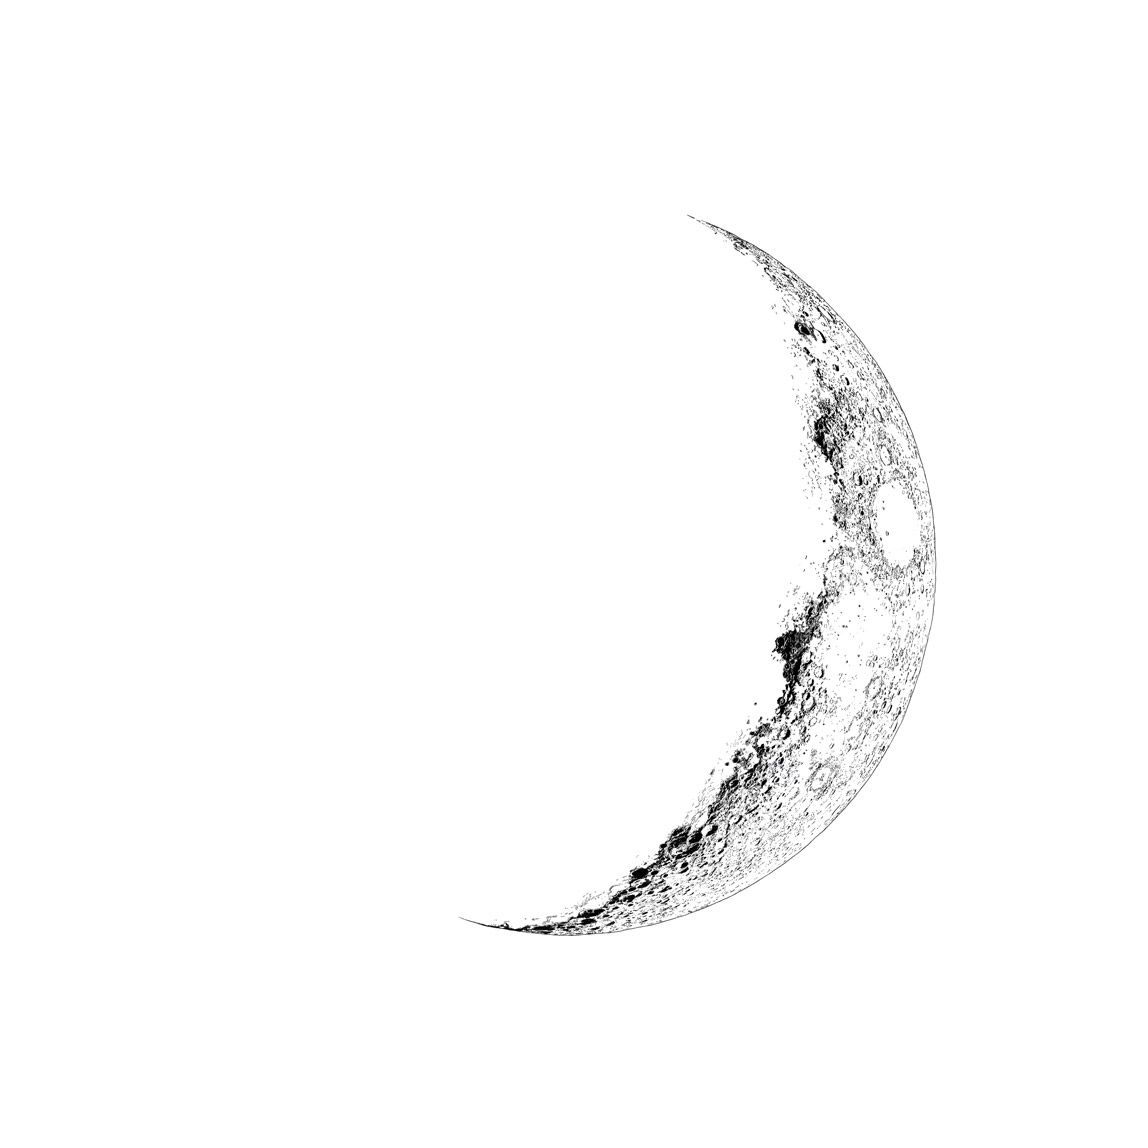
\includegraphics[width=\paperheight]{moon.jpg}
  }%
}
\null
\BgThispage

\end{document}
